%\documentclass[12pt,letter]{report}
\documentclass[12pt,oneside,openany,letter]{book}
\usepackage[colorlinks=true,bookmarksnumbered,linktocpage,pdftex]{hyperref}
\usepackage{hyperref}
\usepackage[activeacute,spanish]{babel}
\usepackage[utf8]{inputenc}
\usepackage{amsmath}
\usepackage{float}
\usepackage{epsfig}
\usepackage{graphicx}
\usepackage{titlesec}
\usepackage{multirow}
\usepackage{graphicx}
\usepackage{caption}
\usepackage{subcaption}
\usepackage{color}
\usepackage{calc}
\usepackage[nottoc]{tocbibind}
\usepackage{titletoc}
\usepackage{capt-of}
\usepackage{verbatim}
\usepackage[titletoc,title]{appendix}
\usepackage[left=3cm, right=3cm,top=3cm, bottom=2.5cm]{geometry}

\newcommand{\bigrule}{\titlerule[1mm]}
\definecolor{c1}{rgb}{0,0.5,0}
\definecolor{c2}{rgb}{0.9,.0,0}
\definecolor{c3}{rgb}{.465,.535,.605}%color del panel
\definecolor{c4}{rgb}{.6,.6,.6}%color de los botones del panel

\hypersetup{linkcolor=blue}                         
\hypersetup{citecolor=red}

%%%%FORMA DE LOS CAPITULOS SECCIONES...ETC%%%%%%

%========================================
% Formato de capítulos y secciones
%\newcommand{\esp}{\rule{0in}{3ex}} %para crear espacios en las tablas
\usepackage{titlesec}
\titleformat{\section}[hang]{\bfseries} {\Large\thesection}{12pt}{\Large}[{\titlerule[0pt]}]
 % Para hacer una línea debajo de cada sección
\titleformat{\chapter}[display] % cambiamos el formato de los capítulos
{\bfseries\Huge} % por defecto se usarán caracteres de tamaño \Huge en negrita
{ \filleft % texto alineado a la derecha
 \Large\chaptertitlename\ % "Capítulo" o "Apéndice" en tamaño \Large en lugar de \Huge
 \Large\thechapter} % número de capítulo en tamaño \Large
{0mm} % espacio mínimo entre etiqueta y cuerpo
{\filleft} % texto del cuerpo alineado a la derecha
[\vspace{0.5mm} \bigrule] % después del cuerpo, dejar espacio vertical y trazar línea horizontal gruesa



\setlength{\parskip}{10pt} %espacio entre párrafos
\makeatletter
\newcommand\figcaption{\def\@captype{figure}\caption}
\makeatother


%%%%%%%%%% NEW COMANDS %%%%%%%%%%%%%%%%%%%%%%%%%%%%%%%%%%%%%%%%%55

%%%%%%%%%%%%%%%%%%%%%%%%%%%%%%%%%%%%%%%%%%%%%%%%%%%%%%%%%%%%%%%%%%%%%%%%%%%%%%
\parindent0cm %Sangria
\parskip0.5cm %Espacio entre prrafos.
\baselineskip0.5cm
\begin{document}
\begin{titlepage}
%\bce
\centering {\Large\textbf{ {\sc Estimación de la respuesta generada por el detector MuTe al paso de partículas cargadas}}}\vfill
\centering {\Large \sc Adriana Carolina Vásquez Ramírez}\\
\vfill
\centering {\Large Universidad Industrial de Santander\\Facultad de
Ciencias\\Escuela de F\'{i}sica\\Bucaramanga\\2018}
\end{titlepage}
\begin{titlepage}
%\bce
\centering {\Large {\sc  Estimación de la respuesta generada por el detector MuTe al paso de partículas cargadas}}

\vfill

\centering {\Large \sc Adriana Carolina Vásquez Ramírez}

\vfill

\centering {\Large \textbf{Director:} Ph.D. Luis A. Núñez}

\centering {\Large \textbf{Codirector:} M.Sc. Mauricio Suárez-Durán}


\vfill

\centering {\Large {Trabajo de grado para optar al t\'itulo de Mag\'ister en Física}}


\vfill
{\Large Grupo de Investigaci\'on en Relatividad y Gravitaci\'on - UIS} \\
{\Large Grupo Halley de Astronom\'ia y Ciencias Aeroespaciales} \\

\vfill

\centering {\Large Universidad Industrial de Santander\\Facultad de
Ciencias\\Escuela de F\'{i}sica\\2018}
\end{titlepage}
\newpage
\setcounter{page}{3}
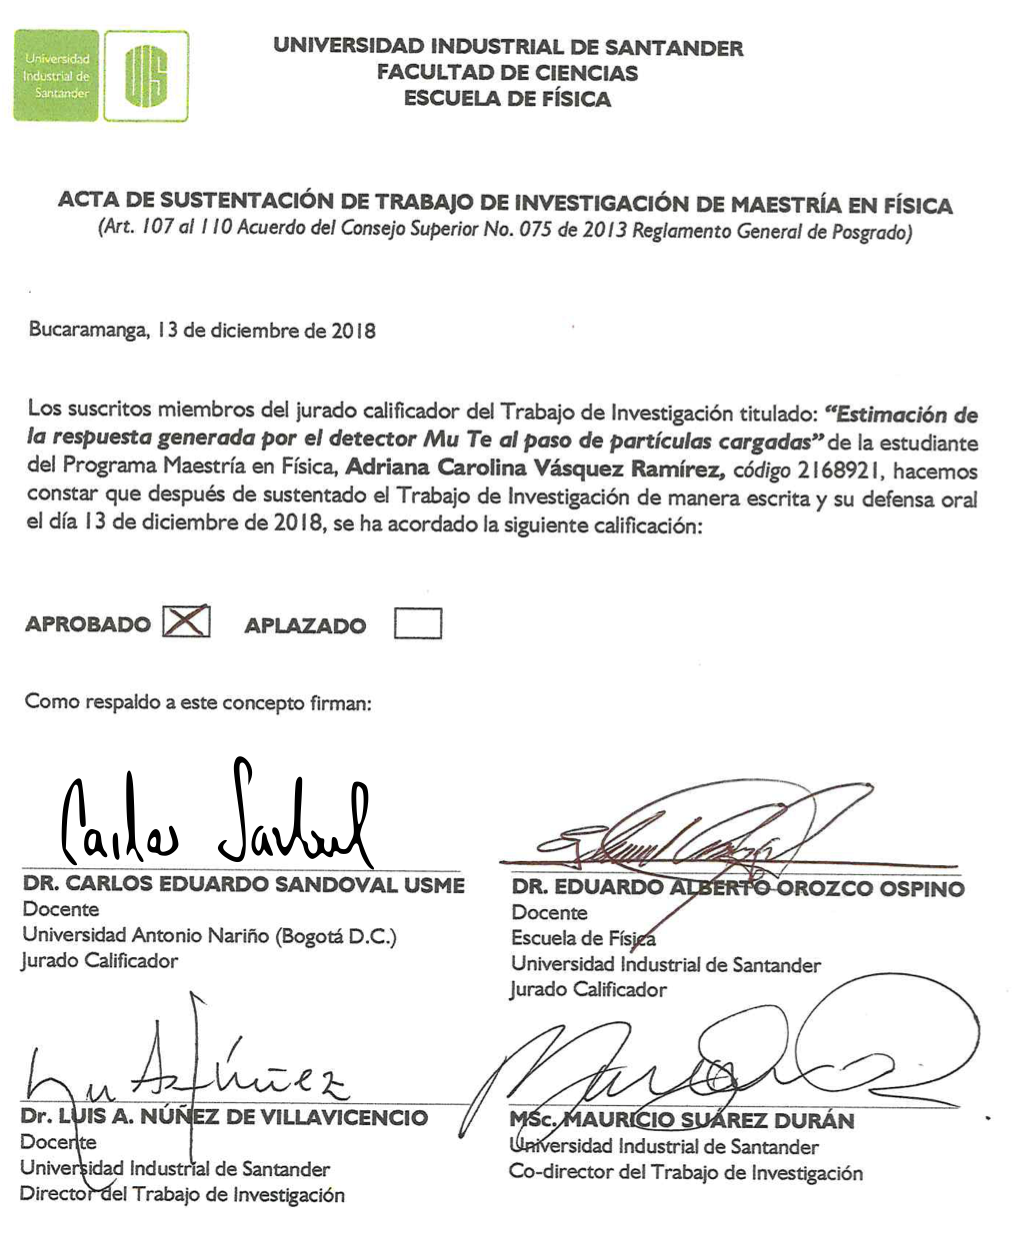
\includegraphics[scale=1]{ACTA.png}
\newpage

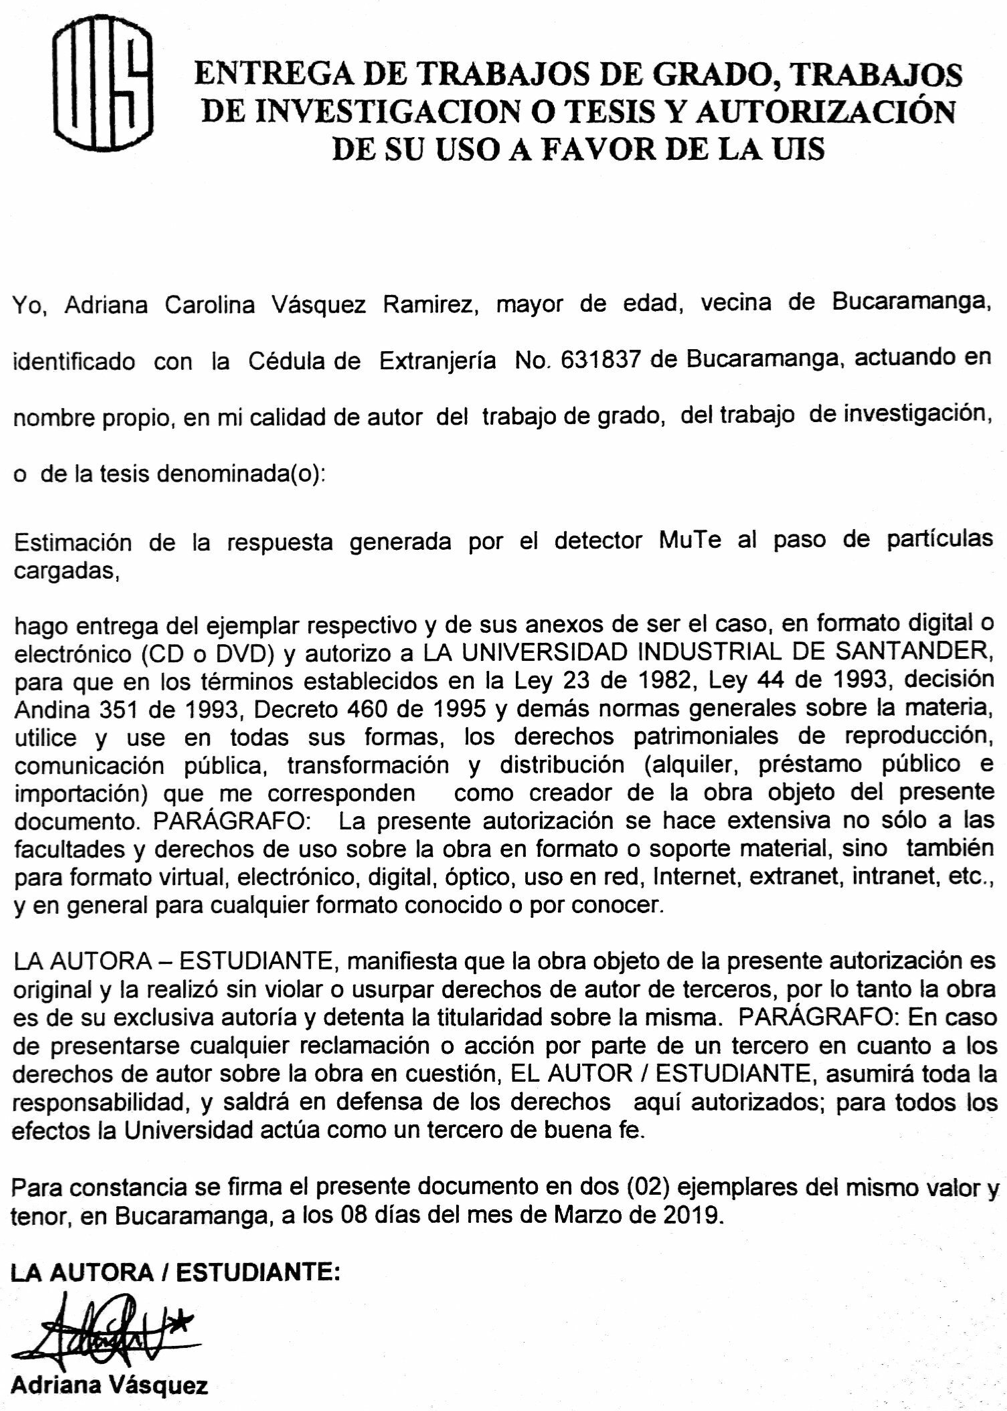
\includegraphics[scale=0.9]{carta.png}
%%%%%%%%%%%%%%%%%%%%%%%%%%%%%%%%%%%%%
%%%%%%%%% dedicado a %%%%%%%%%%%%%%%%
%%%%%%%%%%%%%%%%%%%%%%%%%%%%%%%%%%%%%
\newpage
%\pagenumbering{Roman}
%\pagestyle{empty}
\begin{flushright}
\vspace{5 cm}
\textit{A Anouk V\'asquez \\
y a todas las Aspigirls,\\
%Dedicado a todos los aspies\\ 
para que nunca se rindan \\
y encuentren su lugar en este mundo.\\
En memoria de mi abuelo,\\
Ram\'on V\'asquez.\\}

\vspace{0.5cm}

\end{flushright}

\chapter*{Agradecimientos}

Un d\'ia vas caminando ensimismada, concentrada en los pensamientos que te acompa\~nan d\'ia a d\'ia, las preocupaciones y la rutina que tanto te abruman, pero de repente te proponen un trabajo. Aparece una idea\footnote{Luis N\'u\~nez} que quiere ser desarrollada. Sabes bien que sola no ser\'a f\'acil, pero tambi\'en has aprendido que en colaboraci\'on\footnote{Grupo Halley} se logran los objetivos planteados. 

Es complicado ser el nuevo miembro de un grupo. Al principio todos te observan por ser la desconocida. Las personas suelen rechazar lo nuevo por miedo, es una forma de autodefensa. Queda de tu parte hacerles ver que no eres la amenaza, que si te dejan entrar a la tribu podr\'as serles de mucha utilidad. Este concepto\footnote{Orlando V\'asquez}, del cual no soy autora, me ha ayudado a perseverar y a dominar los miedos que a veces no me permiten socializar para trabajar en conjunto. Pero hay que ver que no soy la \'unica, parece que en este mundo de cient\'ificos habemos muchos a los que nos cuesta la integraci\'on social. Ha sido de gran ayuda encontrar mis pensamientos y actitudes en otras personas. En este tiempo fui a varias escuelas de Física donde conoc\'i personas muy agradables\footnote{Mariel Estevez} \footnote{Orazio Zapparrata}. Entonces entendí que la importancia de estos encuentros reside más en la construcción de redes sociales científicas que en la adquisición de conocimientos. Aprend\'i que la ciencia se hace en conjunto y que en aislamiento es m\'as lento el progreso. Siempre puedes aprender mucho de los dem\'as y ellos de t\'i, es decir, se vuelve a reafirmar uno de esos dichos populares: ``Dos cabezas piensan mejor que una".

Y as\'i, pensando con varias cabezas\footnote{Mauricio Su\'arez, Andrei Jaimes, Rolando Calder\'on, David Sierra}, he logrado alcanzar los objetivos planteados en esta investigaci\'on. Todo esto dentro de un lugar ameno\footnote{Universidad Industrial de Santander} que aporta los recursos necesarios para el desarrollo de las ideas.

Hay d\'ias que el dolor de patria\footnote{Venezuela} no me deja avanzar, la injusticia social es algo que me desespera y a veces creo que es el motivo principal para abrigarme con las ciencias exactas. Sin embargo, el calor familiar\footnote{Mar\'ia Ram\'irez}, ese que con el que hemos crecido\footnote{Mis queridos hermanos: Rhony V\'asquez, Ana Bell V\'asquez, Lindys V\'asquez}, es capaz de transmitirse por las redes de comunicaci\'on, para levantarte y darte un motivo para seguir luchando. No me pregunten c\'omo ocurre este fen\'omeno, pues f\'isicamente no tiene explicaci\'on. A\'un as\'i necesitamos el contacto directo con otras personas, y es ah\'i cuando aparecen familias\footnote{Quinta Sofia: Ysabel Brice\~no, H\'ector Rago, Juli\'an N\'u\~nez, Yankady Rebolledo} que te acogen como un miembro m\'as\footnote{Jose Herrera y Chepe}. Amigos que se preocupan\footnote{Amanda Balaguera} \footnote{Alejandra Vesga} \footnote{Arturo N'u\~nez} por tu bienestar y tu avance laboral. As\'i, los seres humanos vamos construyendo nuestra red de apoyo\footnote{Dami\'an Neri} para seguir avanzando en lo que nos proponemos. Sabemos que siempre est\'a la persona especial que mejor te conoce, que va hombro a hombro contigo y te anima cada d\'ia a luchar por tu futuro\footnote{Ricardo Choy}. Tambi\'en est\'an las personas que te ayudan de forma indirecta\footnote{Mar\'ia Chuecos} \footnote{Leonardo Choy} sin imaginarse que est\'an contribuyendo al avance de tu trabajo\footnote{Familia Escalante}.

El lector se preguntar\'a el motivo de este relato, cuando un t\'itulo as\'i deber\'ia estar seguido de una lista de personas con la palabra \textit{gracias} al inicio de cada una. Me he tomado la libertad que me ofrece este espacio para descargar toda la parte \textit{humana} de la que nuestros reportes cient\'ificos a veces carecen y que tanto nos reprochan. Hace poco hablaba con un estudiante de doctorado\footnote{Oscar Barragan} sobre la importancia de la divulgación científica. Según su experiencia, esto ayuda a que las personas se acerquen más al mundo de la descripción de la naturaleza, sin percibirlo como una exclusividad de las mentes brillantes. Como física, me he comprometido a compartir lo poco que sé a aquellos que me preguntan y como mujer de ciencias, a inspirar a otras compañeras que decidieron andar por estos caminos rompiendo los estereotipos que reprimen nuestras ganas de aprender.

Hoy sigo caminando sumida en mis pensamientos, pero cuando veo esta lista despierto, no estuve sola, me acompa\~naron m\'as de 24 personas a las que hoy agradezco por inspirarme a escribir otra historia. 

``Seguimos'', como dir\'ia L.N.\footnote{H\'ector Hern\'andez}






\tableofcontents
\listoffigures
%\listoftables
%\newpage
\chapter*{Resumen}
{\footnotesize \textbf{T\'ITULO:} ESTIMACI\'ON DE LA RESPUESTA GENERADA POR EL DETECTOR MUTE AL PASO DE PART\'ICULAS CARGADAS.\\
\textbf{AUTORA:} ADRIANA CAROLINA V\'ASQUEZ RAM\'IREZ.\\
\textbf{PALABRAS CLAVE:} Detector de muones, hodoscopio, centelladores, WCD, muongraf\'ia.\\
El Telescopio de Muones (MuTe) es un detector h\'ibrido que est\'a compuesto por dos detectores independientes: un hodoscopio de centelladores pl\'asticos, para estimar la direcci\'on de arribo de las part\'iculas; y un detector Cherenkov de agua, para diferenciar entre las componentes de las cascadas atm\'osfericas extendidas (EAS). Las EAS son producidas por la interacci\'on de los rayos c\'osmicos con los n\'ucleos que conforman la atm\'osfera terrestre. Est\'an compuestas de part\'iculas secundarias clasificadas como: la componente electromagn\'etica, la mu\'onica y la hadr\'onica. En este trabajo se presentan los resultados obtenidos para proponer el trigger de detecci\'on de muones en el MuTe, basado en un conjunto de condiciones que deben ocurrir, en el hodoscopio y en el WCD, en un orden espec\'ifico. Para esto se simuló la respuesta de los detectores de centelleo que conforman el hodoscopio y se obtuvo que los muones de 3 GeV deben generar m\'as de 37 fotoelectrones en los fotosensores del centellador. Esto equivale a depositar alrededor de 2.08 MeV. Por lo tanto, para determinar la direcci\'on de arribo de una part\'icula, \'esta debe generar 37 fotoelectrones en dos barras centelladoras del panel frontal y luego en el panel trasero, para finalmente ser clasificada en el WCD. Para analizar la respuesta del WCD se emple\'o la unidad de medida VEM (Mu\'on Vertical Equivalente) y se obtuvo que el n\'umero de fotoelectrones generados est\'a alrededor de 203. La energ\'ia depositada correspondiente es de 240 MeV aproximadamente. Por otra parte, se realizaron las simulaciones correspondientes a la respuesta del WCD ante el flujo de fondo de rayos c\'osmicos a nivel de la base del volc\'an Cerro Mach\'in. A partir de esto se obtuvo que el histograma de carga presenta dos picos: el primero dominado por la componente electromagn\'etica y el segundo por la componente mu\'onica de las EAS. El primer pico corresponde a 0.024 VEM mientras que el segundo est\'a alrededor de 1.034 VEM, es decir, la diferencia entre ambos permite estimar si la part\'icula incidente es un mu\'on. La metodolog\'ia empleada para el an\'alisis del WCD, dio origen a la codirección de un trabajo de pregrado, que consisti\'o en completar la cadena de simulaciones de la colaboraci\'on LAGO (Latin American Giant Observatory) para estimar la respuesta de detectores Cherenkov de agua a la radiaci\'on c\'osmica. Esta cadena permite obtener el flujo de secundarios corregido por campo geomagnético en el sitio escogido (a trav\'es de los c\'odigos CORSIKA y MAGCOS), para hacerlo incidir sobre el WCD (con el c\'odigo Geant4), y obtener as\'i el histograma del n\'umero de fotoelectrones por part\'icula incidente. Los resultados presentados se emplearán en la calibración del MuTe que ha sido diseñado para realizar la muongrafía de volcanes en Colombia.}

\chapter*{Abstract}

{\footnotesize \textbf{TITLE:} ESTIMATION OF THE RESPONSE GENERATED BY THE MUTE DETECTOR TO CHARGED PARTICLES\\
\textbf{AUTHOR:} ADRIANA CAROLINA V\'ASQUEZ RAM\'IREZ.\\
\textbf{KEY WORDS:} muon detector, hodoscope, scintillators, WCD, muongraphy.\\

The Muon Telescope (MuTe) is a hybrid detector that is composed of two independent detectors: a plastic scintillator hodoscope, to estimate the direction of arrival of the particles; and a Cherenkov water detector, to differentiate between the components of the extended atmospheric showers (EAS). EAS are produced by the interaction between  cosmics rays and the core of the components of the atmosphere. They are composed of secondary particles classified as: the electromagnetic, the muon and the hadron components. In this work we present the results obtained to propose the muon detection trigger in the MuTe, based on a set of conditions that must occur, in the hodoscope and in the WCD, in a specific order. For this, the response of the scintillation detectors that make up the hodoscope was simulated and it was obtained that the 3 GeV muons must generate more than 37 photoelectrons in the scintillator photosensors. This amounts to depositing around 2.08 MeV. Therefore, to determine the direction of arrival of a particle, it must generate 37 photoelectrons in two scintillator bars on the front panel and then on the rear panel, to finally be classified in the WCD. To analyze the response of the WCD, the unit of measurement VEM (Muon Vertical Equivalent) was used and it was obtained that the number of photoelectrons generated is around 203. The corresponding deposited energy is approximately 240 MeV. On the other hand, simulations were carried out corresponding to the response of the WCD to the background flux of cosmic rays at the base level of the Cerro Machin volcano. From this it was obtained that the charge histogram presents two peaks: the first dominated by the electromagnetic component and the second by the muon component of the EAS. The first peak corresponds to 0.024 VEM while the second one is around 1.034 VEM, that is, the difference between the two allows estimating if the incident particle is a muon. The methodology used for the analysis of the WCD, gave rise to the co-direction of an undergraduate work, which consisted in completing the chain of simulations of the collaboration LAGO (Latin American Giant Observatory) to estimate the response of Cherenkov detectors of water to cosmic radiation. This chain allows obtaining the secondary flow corrected by the geomagnetic field at the chosen site (through the CORSIKA and MAGCOS codes), to make it impact on the WCD (with the Geant4 code), and thus obtain the histogram of the number of photoelectrons per incident particle. The results presented will be used in the calibration of the MuTe, which has been designed to perform the volcano muongraphy in Colombia.}



%%%%%%%%%%%%%%%%%%%%%%
%%%%% CHAPTER 1  %%%%%
%%%%%%%%%%%%%%%%%%%%%%
\chapter{Introducción}\label{cap1}
En el marco de la Física de Altas Energías, se tiene la clasificaci\'on de las part\'iculas elementales en torno a sus propiedades f\'isicas. Los muones pertenecen a la familia de leptones y su masa en reposo es cerca de 200 veces la de un electrón \cite{Beringer-etal2012}. Estas part\'iculas pierden poca energía al interactuar con la materia, por lo que tienen un alto poder penetrante en los materiales. A partir de esta caracter\'istica se ha originado la muongraf\'ia, que consiste en medir la atenuaci\'on del flujo de muones que ha atravesado una estructura, respecto al flujo conocido previamente a la interacci\'on. Esta diferencia en el flujo est\'a asociada a la distribuci\'on de densidades en los materiales \cite{jourde2013experimental}. 

La interacción de los rayos cósmicos con los núcleos de los elementos de la atmósfera terrestre da origen a las lluvias atmosféricas extendidas (EAS). Las partículas secundarias producidas en las EAS se clasifican en tres componentes: la muónica, la electromagnética y la hadrónica. El flujo de muones empleado en la muongrafía proviene de estas interacciones y presenta un amplio espectro de energías \cite{Asorey-phd2012}.

Estas part\'iculas secundarias sólo pueden ser detectadas a través de su interacción con la materia, entonces cada proceso de interacción se puede tomar como base para diseñar un detector \cite{ClausBoris}. La ionización y la excitación son los  procesos principales utilizados en los detectores de partículas cargadas. Dependiendo de sus propiedades físicas, geométricas y materiales, pueden dar información sobre la masa, la carga, la trayectoria, el tiempo de vuelo y otras características de las partículas subatómicas \cite{spurio2014particles}. 

La muongrafía se ha desarrollado en distintos proyectos como el MU-RAY \cite{Anastasio-etal2013}, el ToMuVol \cite{carloganu2013towards} y el DIAPHANE \cite{lesparre-etal2010}, para estimar los perfiles de densidad del interior de ciertos volcanes, como el Mt. Sukuba \cite{Nagamine-etal1995}, Mt. Asama \cite{Tanaka-etal2001hi}, \cite{Tanaka-etal2007epsl}, \cite{Tanaka2007}, Mt. Satsuma-Iwojima, Mt.West Iwate \cite{Tanaka-etal2005nimprs}, y el domo de lava Showa-Shinzan \cite{Tanaka-etal2007grl}. Adem\'as, se han establecido las condiciones para la aplicación de la muongrafía en otros volcanes, como el Mt. Vesuvio \cite{Beauducel-etal2008}, en el domo de lava del Mt. Usu \cite{Tanaka-Yokoyama2008} y en el Mt. Satsuma-Iwojima \cite{Tanaka-etal2009}. La muongrafía axial tridimensional se ha realizado en el Mt Asama \cite{Tanaka-etal2010wol}, Puy de Dome \cite{carloganu2013towards}, \cite{Carloganu2011}, \cite{Portal-etal2013}, el volcán La Soufriere de Guadaloupe \cite{Lesparre-etal2012-gji}, \cite{jourde2013experimental} y el Mt Etna \cite{Carbone-etal2014}. Esta t\'ecnica tambi\'en se ha empleado para monitorear el movimiento del magma, en las erupciones del Mt. Asama y en la erupción del Satsuma-Iwo Jima \cite{Tanaka-etal2014nc}.  

El proyecto MuTe se ha creado dentro de este contexto, para el estudio del interior de estructuras volc\'anicas en Colombia empleando la técnica de la muongrafía. El Telescopio de Muones que se ha diseñado est\'a compuesto por dos detectores: un hodoscopio de barras centelladoras, para estimar la trayectoria de las partículas; y un detector Cherenkov de agua, para diferenciar entre la componente mu\'onica y la electromagn\'etica de las EAS \cite{SuarezDuran2016}. En este sentido, la respuesta del detector h\'ibrido MuTe, se basa en determinar el n\'umero de fotoelectrones producidos en los fotosensores de ambos detectores, al paso de part\'iculas cargadas. Para estimar esta respuesta se utiliz\'o la herramienta Geant4, que se compone de un conjunto de c\'odigos para la simulaci\'on de la interacci\'on de part\'iculas de alta energ\'ia con la materia, con un alto nivel de detalle \cite{Geant4}. El Geant4 ha sido desarrollado por el Consejo Europeo para la Investigaci\'on Nuclear (CERN), para la simulaci\'on y el an\'alisis de la respuesta de sus detectores, y se ha puesto a disposici\'on de los usuarios para el desarrollo de sus investigaciones alrededor de la f\'isica de altas energ\'ias, f\'isica nuclear y aceleradores, ciencias m\'edicas y espaciales. 

En lo que sigue se describirá la técnica de muongrafía de volcanes y algunos detectores que se han utilizado alrededor del mundo. En el capítulo \ref{cap3} se muestra el funcionamiento del hodoscopio del MuTe, y su respuesta ante muones monoenergéticos. La respuesta del detector Cherenkov de agua (WCD), ante muones y electrones, se expone en el capítulo \ref{cap4}, así como los resultados obtenidos para el flujo de partículas secundarias a nivel del Volcán Cerro Machín. En el capítulo \ref{cap5} se propone el trigger de detecci\'on de muones del MuTe, basado en la correlaci\'on de los resultados obtenidos para el hodoscopio y para el WCD. Finalmente se presentan las conclusiones de esta investigación en el capítulo \ref{cap6}.

%%%%%%%%%%%%%%%%%%%%%%
%%%%% CHAPTER 2  %%%%%
%%%%%%%%%%%%%%%%%%%%%%
\chapter{La muongrafía de volcanes y el Proyecto MuTe}\label{cap2}
%%%%%%%%%%%%%%%%%%%%%%%%%%%%%%%
%%%%%%%%%   Section   %%%%%%%%%
%%%%%%%%%%%%%%%%%%%%%%%%%%%%%%%


\section{La muongrafía de volcanes}
La tomografía de muones (o muongrafía) es una t\'ecnica que se basa en medir la atenuación de un flujo de muones que atraviesa estructuras geológicas y antr\'opicas, para determinar la distribuci\'on de densidades en su interior \cite{jourde2013experimental}. Los muones provienen del decaimiento de piones y kaones, que se producen a través de la interacci\'on de los rayos cósmicos con los n\'ucleos de la alta atmósfera terrestre \cite{Grieder2001}. La energ\'ia de estas part\'iculas comprende un amplio espectro, pero s\'olo aquellos muones con altas energías ($\sim 100$GeV) tienen la capacidad de atravesar cientos de metros de roca. Adem\'as son las part\'iculas cargadas m\'as abundantes que llegan al nivel del mar, debido a su alto poder penetrante (s\'olo pierden alrededor de 2 GeV al recorrer toda la atm\'osfera)  \cite{spurio2014particles}. Otra ventaja de los muones es su facilidad de detecci\'on respecto a otras part\'iculas, a partir de diferentes t\'ecnicas como la ionizaci\'on, excitaci\'on y el efecto Cherenkov \cite{Marteau-etal2012}.

Los muones llegan constantemente a la superficie terrestre con diferentes direcciones y energ\'ias \cite{Asorey-phd2012}, permitiendo desarrollar aplicaciones espec\'ificas en torno a esto. Por ejemplo, los muones verticales arriban con una tasa de 1$\mu$/cm$^2$min y energ\'ias de unos pocos GeV \cite{nagamine_2003}. El uso potencial de este flujo fue reconocido por primera vez por Alvarez \cite{Alvarez-etal1970} en 1970,  para explorar la estructura interna de pir\'amides con el objetivo de encontrar cámaras ocultas. En diciembre del 2017 se anunci\'o el descubrimiento de un gran espacio vac\'io en la pir\'amide de Khufu, mediante la observaci\'on de muones provenientes de los rayos c\'osmicos \cite{morishima2017discovery}. Los resultados fueron obtenidos con detectores de l\'aminas de emulsiones nucleares, instaladas en el interior de una c\'amara de la pir\'amide, y luego fueron confirmados con hodoscopios de centelladores y con detectores gaseosos, ubicados fuera de la estructura. 

Por otro lado, est\'an los muones que llegan casi horizontalmente a lo largo de la superficie de la tierra, con un ángulo cenital $\theta$ ligeramente inferior a $90^{\circ}$, que tienen una tasa menor a los verticales pero sus energías son más altas (superiores a algunos cientos de GeV) \cite{nagamine_2003}. \'Estos se pueden utilizar para escanear la estructura interna de objetos verdaderamente gigantescos como los volcanes, siempre que el flujo de muones sea razonablemente alto en el sitio de observaci\'on y que se cuente con el sistema de detección requerido \cite{nagamine_2003}. En este caso es esencial filtrar los datos producidos por otras part\'iculas, es decir, por la componente débil de los rayos cósmicos: las cascadas de electrones, positrones y fotones \cite{nagamine_2003}.

La muongrafía usa los mismos principios básicos de una radiografía médica: midiendo la atenuación del haz de muones (en lugar de rayos X) cuando atraviesan la roca (en lugar del tejido humano) con un detector sensible a partículas cargadas \cite{Marteau-etal2012}, se obtiene una imagen del objeto donde los diferentes tonos están asociados a diferentes densidades. Así, la opacidad ($\varrho$) de una estructura volcánica se puede obtener comparando el flujo de muones después de atravesar el volcán, $\Phi_v$, y el flujo incidente a cielo abierto, $\Phi_0$, sobre el detector. Esta opacidad se define en t\'erminos de la densidad del material, como
\begin{equation}
\varrho \equiv \int_{L} \rho(\xi) d\xi \,\,\, = \bar{\rho}\times L \,\,\,  [\text{kg m}^{-2}],
\end{equation}
donde $L$ es la distancia total recorrida por los muones en la roca y $\bar{\rho}$ es la densidad promedio a lo largo de esta trayectoria \cite{Marteau-etal2012}.

Conociendo la energ\'ia perdida por los muones en la roca, se puede determinar la energ\'ia m\'inima, $E_{min}$, necesaria para recorrer cierta opacidad, a partir de la ecuaci\'on,
\begin{equation}
E_{min}(\varrho)=\int^{\varrho}_{0} \frac{dE}{d\varrho} d\varrho +E_{\mu},
\end{equation}
donde $E_{\mu}$ es la energ\'ia del mu\'on en reposo \cite{lesparre-etal2010}. Esta p\'erdida de energía se da por diferentes procesos físicos, como la ionizaci\'on, el Bremsstrahlung, las interacciones nucleares y la producción de pares, $e^-e^+$, dada por la ecuaci\'on, 
\begin{equation}
- \dfrac{d E}{d \varrho} = a(E)+b(E)E \,\,\, [\text{MeV g}^{-1}\text{cm}^2],
\end{equation}
donde las funciones $a(E)$ y $b(E)$ representan las p\'erdidas por ionizaci\'on y por radiaci\'on, respectivamente \cite{Marteau-etal2012}. 

El flujo integral de muones, $I_{\mu}(E_{min}(\varrho), \theta)$, con la energía suficiente para atravesar un material de opacidad conocida, en un ángulo cenital, $\theta$, es 
\begin{equation}
I_{\mu}(E_{min}(\varrho), \theta)=\int_{E_{min}(\varrho)}^{\infty}\Phi(E,\theta)dE.
\end{equation}
Inversamente, si se desconoce la opacidad, ésta se puede determinar midiendo el flujo de muones emergentes con cierto ángulo cenital $I_{\mu}(\theta)$. La intensidad relativa de muones atmosféricos transmitida a través del volcán, con respecto a los que vienen directamente del cielo abierto, ${I_{\mu}(0, \theta)}$, es
\begin{equation}
n(\theta) = \frac{I_{\mu}(\varrho, \theta)}{I_{\mu}(0, \theta)}.
\end{equation}
Entonces, midiendo $n$ en un \'angulo $\theta$ conocido, se puede determinar $\varrho(\theta)$ \cite{nagamine_2003}. En la figura \ref{muon_intensity}, se muestra como decrece la intensidad de muones con el aumento del espesor, $X$, de una roca con densidad conocida, $\rho=$2.5 g/cm$^3$, a diferentes \'angulos cenitales. Extendiendo este estudio a dos dimensiones, se puede medir $n(\theta, \phi)$ y a través de estos datos se obtienen imágenes del interior de volcanes activos, como se muestra en la figura \ref{perfil}.

\begin{figure}[h]
\begin{subfigure}{0.4\textwidth}
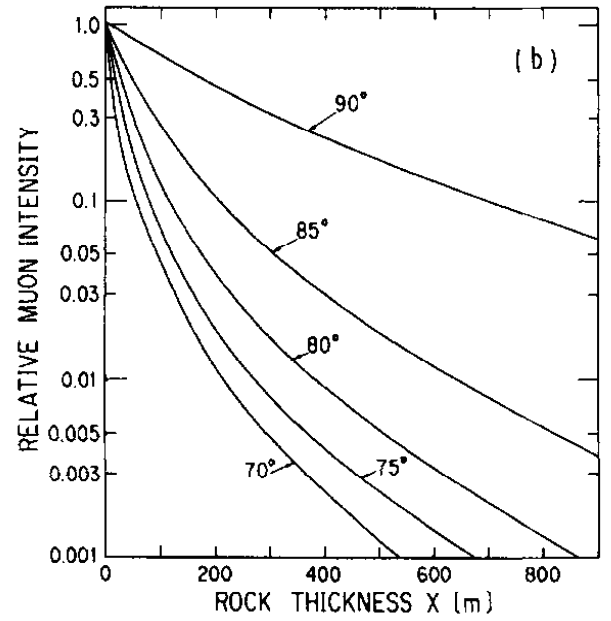
\includegraphics[width=\textwidth]{muon_intesity.png}
\caption{}
\label{muon_intensity}
\end{subfigure}
\begin{subfigure}{0.6\textwidth}
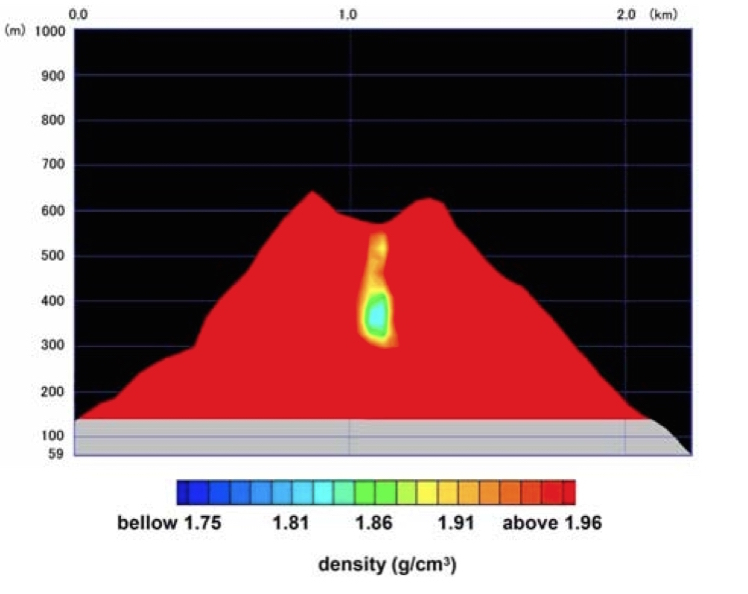
\includegraphics[width=\textwidth]{images/perfil.jpg}
\caption{}
\label{perfil}
\end{subfigure}
 \caption[Intensidad de muones que penetran una roca con densidad conocida]{(a) Intensidad relativa de un flujo integrado de muones que atraviesan una roca con densidad de 2.5 g/cm$^3$ a diferentes ángulos cenitales \cite{Nagamine-etal1995}. Se puede observar que la intensidad relativa de muones disminuye conforme aumenta la cantidad de roca atravesada por las partículas. (b) Perfil de densidad promedio dado por el resultado del procesamiento de datos del flujo de muones atmosféricos en el Mt. Iwodake \cite{Tanaka-etal2009}.}
  \label{figura1}
\end{figure}

La resolución espacial de la densidad dada por la muongrafía es mayor que la obtenida por otras técnicas como la perforación, las técnicas geoeléctricas y electromagnéticas, y la gravimetría (\cite{Ambrosi-etal2011}, \cite{Macedonio-Martini2010}, \cite{lesparre-etal2010}, \cite{Tanaka-etal2009}), por lo tanto, la muongrafía permite describir y entender con más detalle la distribuci\'on de densidad y, adem\'as la dinámica de las estructuras volcánicas (\cite{Lesparre-etal2012-gji}, \cite{Jourde-etal2015}, \cite{Nishiyama-etal2014}). La tomografía de muones también se ha aprovechado para distintas aplicaciones como el monitoreo de la estructura interna de una planta nuclear \cite{Fujii-etal2013}, la búsqueda y seguimiento de reservorios geotérmicos \cite{Tanaka-etal2012-gi}, la identificación de materiales desconocidos \cite{Morris-etal2012}, el monitoreo de la concentraci\'on en los almacenamientos de CO$_2$ \cite{Vitaly-etal2012} e incluso la búsqueda de contrabando de material radioactivo \cite{Schultz-etal2004}. 
%el monitoreo de concentración de $\text{CO}_2$ en zonas someras \cite{Vitaly-etal2012}

%%%%%%%%%%%%%%%%%%%%%%%%%%%%%%%
%%%%%%%%%   Section   %%%%%%%%%
%%%%%%%%%%%%%%%%%%%%%%%%%%%%%%%

\section{Hodoscopios empleados para la muongrafía}\label{hodoscopios}
Para el desarrollo de la muongrafía de volcanes es necesario emplear detectores capaces de medir la dirección de arribo de los $\mu$ provenientes del volcán en estudio, para lo que ya se han empleado hodoscopios de diferentes materiales que se muestran en esta secci\'on.

En líneas generales, los hodoscopios son detectores de partículas que consisten de uno o varios paneles de conteo, como se muestra en la figura \ref{hodoscopio_general}, donde la línea recta que conecta los puntos de impacto $(x_i, y_i)$ de la partícula en cada panel, determina su trayectoria, y por lo tanto la dirección de arribo en términos del ángulo cenital $\theta$ y azimutal $\phi$. 

Los proyectos que han desarrollado la muongrafía de volcanes utilizan hodoscopios fundamentados en diferentes técnicas de detección, como los detectores de láminas de emulsiones nucleares (\cite{morishima2017discovery}, \cite{nagamine2016radiography}); los detectores gaseosos como las Cámaras de Platos Resistivos (\cite{sehgal2016simulations}, \cite{fehr2012density}), Micromegas \cite{bouteille2016micromegas}, Cámaras Proporcionales Multi-Hilo (MWPCs) \cite{olah2018high}; y los detectores de Centelleo segmentados (\cite{Fujii-etal2013}, \cite{lesparre-etal2012-gim}, \cite{Tanaka-etal2009}) y continuos (\cite{Nagamine-etal1995}, \cite{aguiar2015geant4}, \cite{tang2016large}). En lo que sigue se describe el principio f\'isico con el que opera cada tipo de detector.

\begin{figure}
\begin{center}
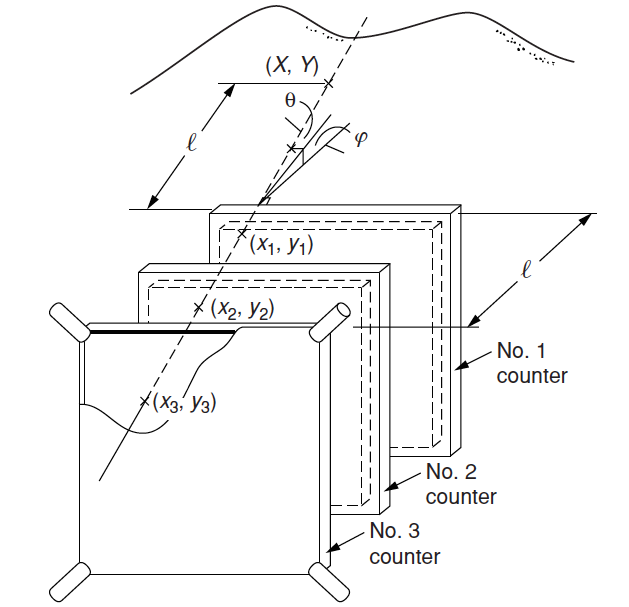
\includegraphics[scale=0.4]{hodoscopio_general.png}
\caption[Esquema general de un hodoscopio]{Esquema general del hodoscopio de centelladores plásticos continuos utilizado para las medidas realizadas en el Mt Tsukuba \cite{nagamine_2003}. A partir de los puntos de impacto ($x_i$, $y_i$) en cada contador, se puede determinar la trayectoria del muón proveniente del volcán y su dirección dada por $\theta$ y $\phi$.}
\label{hodoscopio_general}
\end{center}
\end{figure}

\subsection{Detectores de emulsiones nucleares}
Las pel\'iculas de emulsiones nucleares son empleadas en detectores de part\'iculas cargadas. Estas pel\'iculas, generalmente de cristales de Bromuro de Plata (AgBr), consisten de una base de pl\'astico y un gel de emulsi\'on que los cubre por ambos lados. Los cristales de AgBr en el gel de emulsi\'on nuclear son sensibles a las part\'iculas cargadas, por lo que, despu\'es de que una emulsi\'on se desarrolla, las trayectorias de las part\'iculas cargadas son registradas como l\'ineas tridimensionales de granos de plata \cite{nishiyama2014experimental}, como se muestra en la figura \ref{emulsion}. Estos granos tienen un tama\~no del orden de los submicrones, proporcionando al detector una buena resoluci\'on espacial.
\begin{figure}
\begin{center}
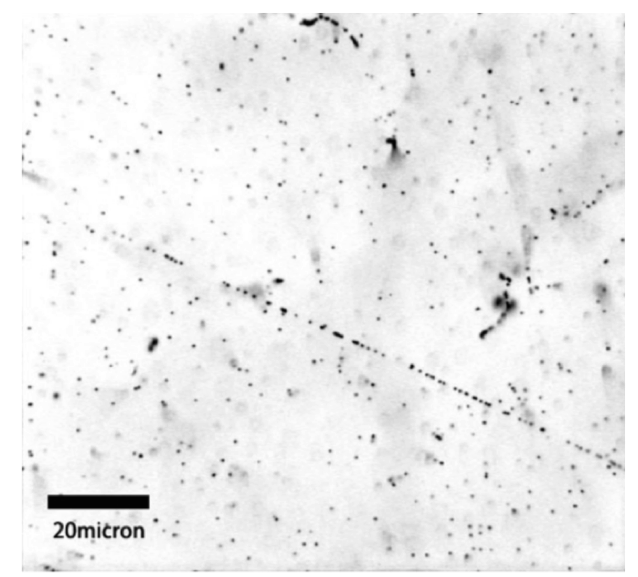
\includegraphics[scale=0.6]{emulsion.png}
\caption[Imagen microsc\'opica de una pel\'icula de emulsi\'on nuclear revelada]{Imagen microsc\'opica de una pel\'icula de emulsi\'on nuclear revelada, se puede observar la l\'inea recta que representa la trayectoria dejada por una part\'icula cargada que ha interactuado con el material. Figura tomada de \cite{nishiyama2014experimental}.}
\label{emulsion}
\end{center}
\end{figure}

A pesar de que los detectores de l\'aminas de emulsi\'on tienen una alta resoluci\'on espacial, son de f\'acil manejo y traslado, y no requieren electricidad para su operaci\'on, presentan una serie de desventajas: el tiempo de vida de las l\'aminas es corto ($\sim$ meses) para realizar un monitero din\'amico del volc\'an, el an\'alisis de datos es costoso debido al procesamiento de las im\'agenes obtenidas, y no es posible hacer un seguimiento temporal de los eventos debido a que se van acumulando en la l\'amina durante el tiempo de exposici\'on \cite{PenaJesus2018}.

\subsection{Detectores gaseosos}
La detecci\'on de part\'iculas cargadas se puede realizar tambi\'en a trav\'es de su interacci\'on con gases ionizados. Este tipo de detector se construye con un gas ionizante contenido entre dos capas de un material conductivo, es decir, entre un \'anodo y un c\'atodo. Al aplicar un alto voltaje entre los electrodos, se genera un campo m\'agnetico dentro del gas, de modo que al paso de una part\'icula cargada se generan pares \'ion-electr\'on. Si el campo el\'ectrico aplicado es lo suficientemente alto, los electrones ser\'an acelerados, desprendiendo m\'as electrones del gas hasta producir un efecto de avalancha. Estos electrones son atra\'idos al \'anodo, generando una corriente el\'ectrica que puede ser registrada como la se\~nal depositada por la part\'icula incidente \cite{PenaJesus2018}. 

En la figura \ref{gaseoso} se muestra el principio de funcionamiento de un detector Micromegas, que se distinguen por poseer una rejilla interna que ayuda a amplificar la avalancha de los electrones. Adem\'as la avalancha es acelerada de tal modo que se disminuye el tiempo de respuesta de estos detectores. 

Los detectores gaseosos permiten obtener una traza temporal de las par\'iculas detectadas, con una resoluci\'on espacial alrededor de los micrones. Sin embargo, la ganancia de los electrodos depende altamente de las variables ambientales, como la presi\'on y la temperatura. Adem\'as, para su funcionamiento \'optimo se requiere de un alto voltaje, lo que se puede traducir en un alto consumo de electricidad en comparaci\'on con los detectores de l\'aminas de emulsi\'on \cite{PenaJesus2018}. 

\begin{figure}
\begin{center}
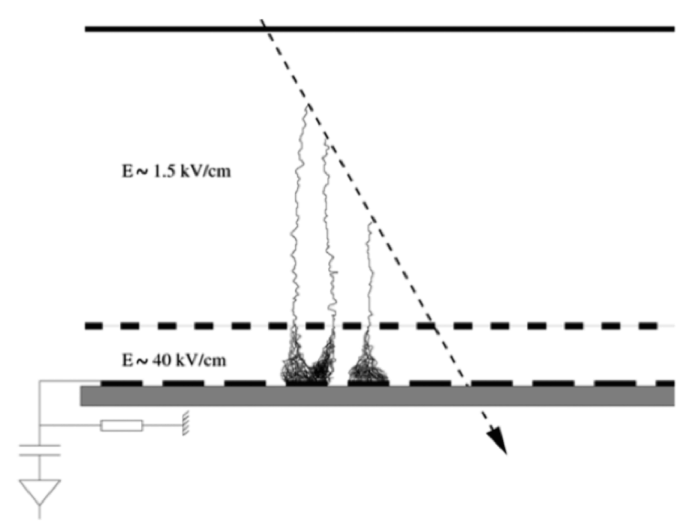
\includegraphics[scale=0.7]{gaseoso.png}
\caption[Principio de funcionamiento de un detector de Micromegas]{Principio de funcionamiento de un detector Micromegas. La trayectoria de la part\'icula incidente est\'a representada por la flecha, donde se observa el desprendimiento de electrones a su paso. La rejilla que caracteriza este detector (l\'inea punteada) amplifica y acelera la avalancha de electrones hacia el \'anodo. Figura tomada de \cite{procureur2018muon}.}
\label{gaseoso}
\end{center}
\end{figure}

\subsection{Detectores de centelleo}
Los detectores de centelleo son m\'as robustos, pues no presentan una alta variaci\'on mec\'anica con las condiciones ambientales; son de f\'acil construcci\'on y a un costo mucho menor que el de los detectores gaseosos y los de emulsi\'on. Sin embargo, su resoluci\'on espacial no es tan buena como la de estos detectores, pues generalmente los segmentos utilizados son del orden de los cent\'imetros. 

El centelleo es un proceso mediante el cual un material emite luz (de un espectro característico) después de haber absorbido radiación. En materiales orgánicos este proceso ocurre cuando las moléculas absorben parte de la energía de la partícula incidente y los electrones del estado base $S_0$ son excitados a un estado $S_1$. Los electrones en el estado $S_1$ se ubican en los estados de vibración $S_{10}$, $S_{11}$, $S_{12}$, $S_{13}$ (ver figura \ref{scintillation_process}). Los tres últimos niveles tienen un exceso de energía en comparación a $S_{10}$ y, al no lograr un equilibrio térmico con su entorno pierden este exceso rápidamente, de modo que la molécula pasa a un estado neto de excitación en $S_{10}$. Al relajarse la molécula, los electrones vuelven a los sub-niveles de $S_0$ ($S_{00}, S_{01}, S_{02}, S_{03}$) emitiendo fotones con un tiempo de decaimiento de algunos nanosegundos. A esto se le conoce como el proceso de fluorescencia y es de principal interés en la detección de partículas. La componente lenta (fosforescencia) es del orden de los microsegundos y corresponde a la emisión de fotones causada por la transición del estado $T_{1}$ al estado $S_0$ \cite{SuarezDuran2016}.

\begin{figure}
\begin{center}
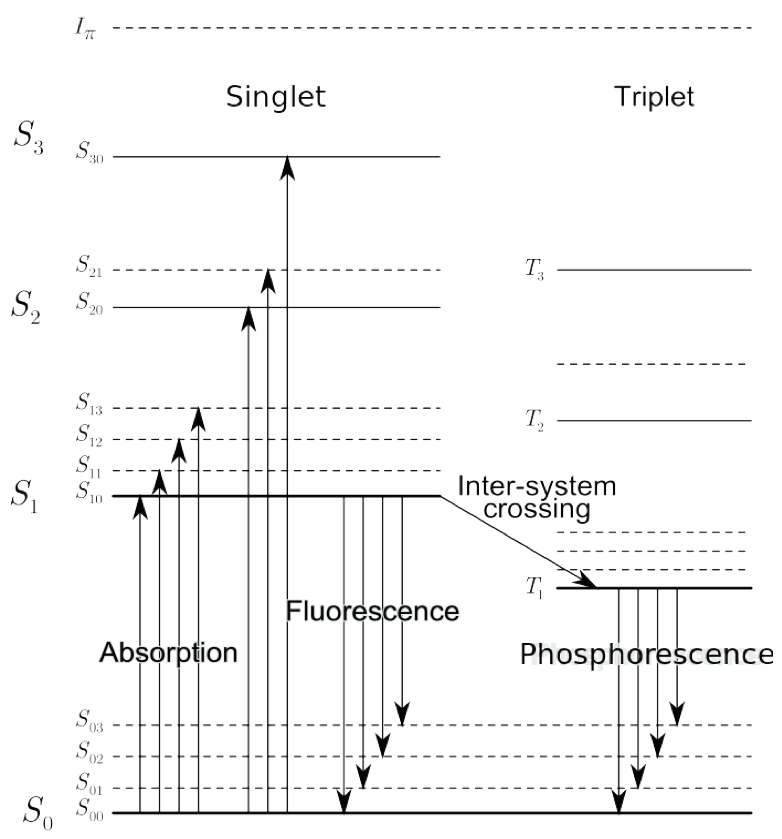
\includegraphics[scale=0.5]{scintillation_process.png}
\caption[Niveles de energía de una molécula orgánica con estructura $\pi$ electrón.]{Niveles de energía de una molécula orgánica con estructura $\pi$ electrón. $S_0$ es el estado fundamental mientras que $S_1$, $S_2$, y $S_3$ son estados de singlete excitados. $T_1$, $T_2$ y $T_3$ son estados de triplete excitados. $S_{00}$, $S_{01}$, $S_{10}$, $S_{11}$, etc. son subniveles vibratorios. Los procesos de fluorescencia y fosforescencia ocurren en distintas transiciones de esos niveles. Figura tomada de \url{ http://www.wikiwand.com/en/Scintillation_(physics)}}
\label{scintillation_process}
\end{center}
\end{figure}

Para la detección de radiación se espera que un centellador ideal cumpla lo siguiente \cite{Gonzalez-maestrando2012}:
\begin{enumerate}
\item Capacidad de conversión de la energía cinética de las partículas cargadas en luz, con alta eficiencia;
\item La conversión debe ser proporcional a la energía depositada;
\item El medio debe ser transparente en el rango de longitudes de ondas emitidas;
\item El tiempo de decaimiento de la luminiscencia producida debe ser corto (fosforescencia);
\item El material debe tener un índice de refracción tal que pueda ser fácilmente acoplado a detectores de fotones.
\end{enumerate}

Los detectores de centelleo generalmente se componen de una barra centelladora con una fibra óptica en su interior, que absorbe parte de la luz producida en la barra al paso de una partícula cargada de alta energía. Los fotones son guiados a trav\'es de la fibra hacia un dispositivo capaz de detectarlos, generalmente se utilizan los Tubos Fotomultiplicadores (PMT) o los Contadores de Fotones Multi-Pixel (MPPC). El esquema de funcionamiento se muestra en la figura \ref{fibra}, donde el SiPM (Silicon Photomultiplier) no es m\'as que un MPPC de silicio. Es importante resaltar que el acople opto-mec\'anico entre la fibra y el MPPC debe ser óptimo para evitar una fuga de fotones. En este detector, los datos de un evento se obtienen a través de una electrónica de adquisición conectada al MPPC, como se observa en la figura \ref{scintillator_scheme}.



\begin{figure}[h!]
\begin{center}

\begin{subfigure}{0.7\textwidth}
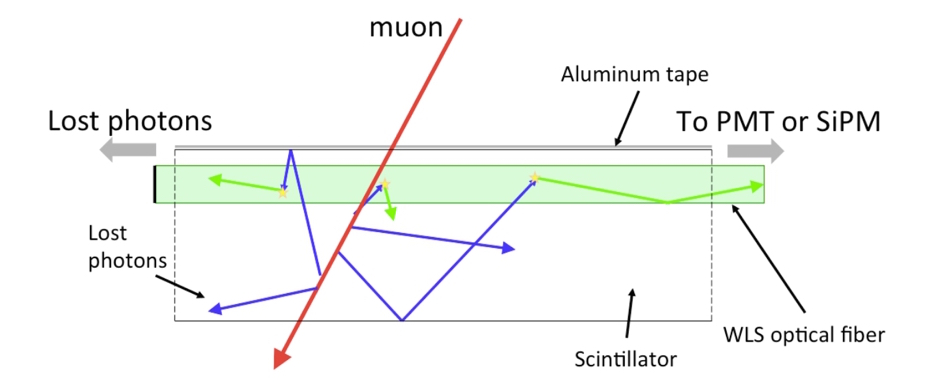
\includegraphics[width=\textwidth]{images/fibra.jpg}
\caption{}
\label{fibra}
\end{subfigure}

\begin{subfigure}{0.55\textwidth}
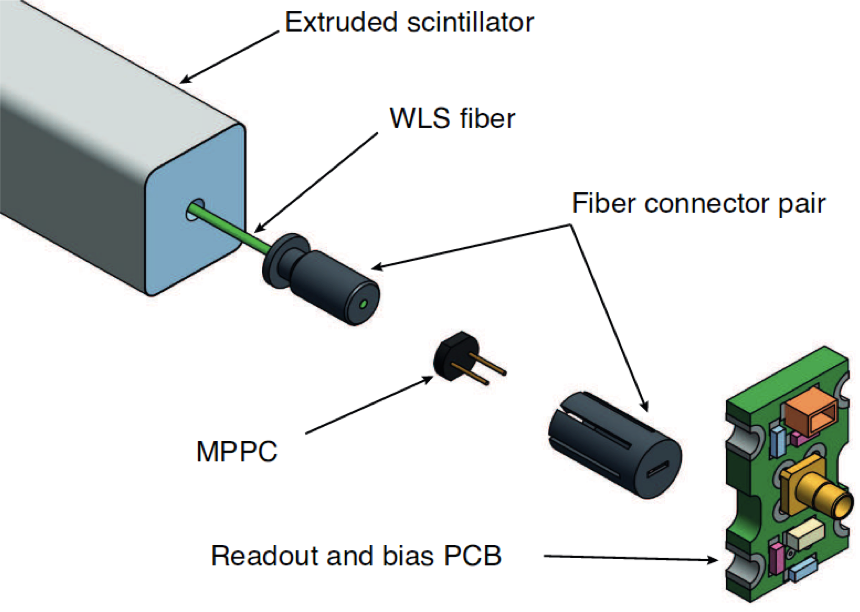
\includegraphics[width=\textwidth]{scintillator_scheme.png}
\caption{}
\label{scintillator_scheme}
\end{subfigure}
\end{center}

\caption[Esquema de funcionamiento de un detector de centelleo]{a) Esquema de funcionamiento de un detector de centelleo que se excita al paso de un muón. La trayectoria del muón está representada por la línea roja, mientras que los fotones producidos por centelleo se identifican con flechas azules. Algunos de \'estos son absorbidos por la fibra y reemitidos en su interior con una longitud de onda $\lambda$ diferente. Ciertos fotones dentro de la fibra viajan hacia el PMT o el SiPM donde serán contados, mientras que otros se pierden hacia el extremo opuesto de la barra \cite{amiga-etal2016}. b) Detalle de los componentes para la conexión de una fibra WLS (Wave Length Shifter) a un MPPC, y a la electrónica de adquisición de un detector de centelleo \cite{soter2014segmented}.}
  \label{scintillator_general}
\end{figure}
En este trabajo nos centraremos en los detectores de centelleo segmentados, los cuales se escogieron para el detector MuTe debido a: su eficiencia, su bajo costo, su desempeño estable con la temperatura y fácil manejo \cite{SuarezDuran2016}. Estos detectores han sido probados en experimentos como MINOS \cite{adamson-etal2002} y AMIGA \cite{amiga-etal2016}. 
%%%%%%%%%%%%%%%%%%%%%%%%%%%%%%%
%%%%%%%%%   Section   %%%%%%%%%
%%%%%%%%%%%%%%%%%%%%%%%%%%%%%%%


\section{El Proyecto MuTe}
El proyecto MuTe\footnote{\url{http://halley.uis.edu.co/fuego}} (Muon Telescope) se origina con el fin de diseñar, construir, calibrar y poner en marcha un dispositivo que permita ejecutar la muongrafía de volcanes en Colombia. Se compone de dos detectores: el hodoscopio de centelladores pl\'asticos, denotado como CP en la figura \ref{mute}, y el detector Cherenkov de agua, WCD en la misma figura. 
\begin{figure}[h!]
    \centering        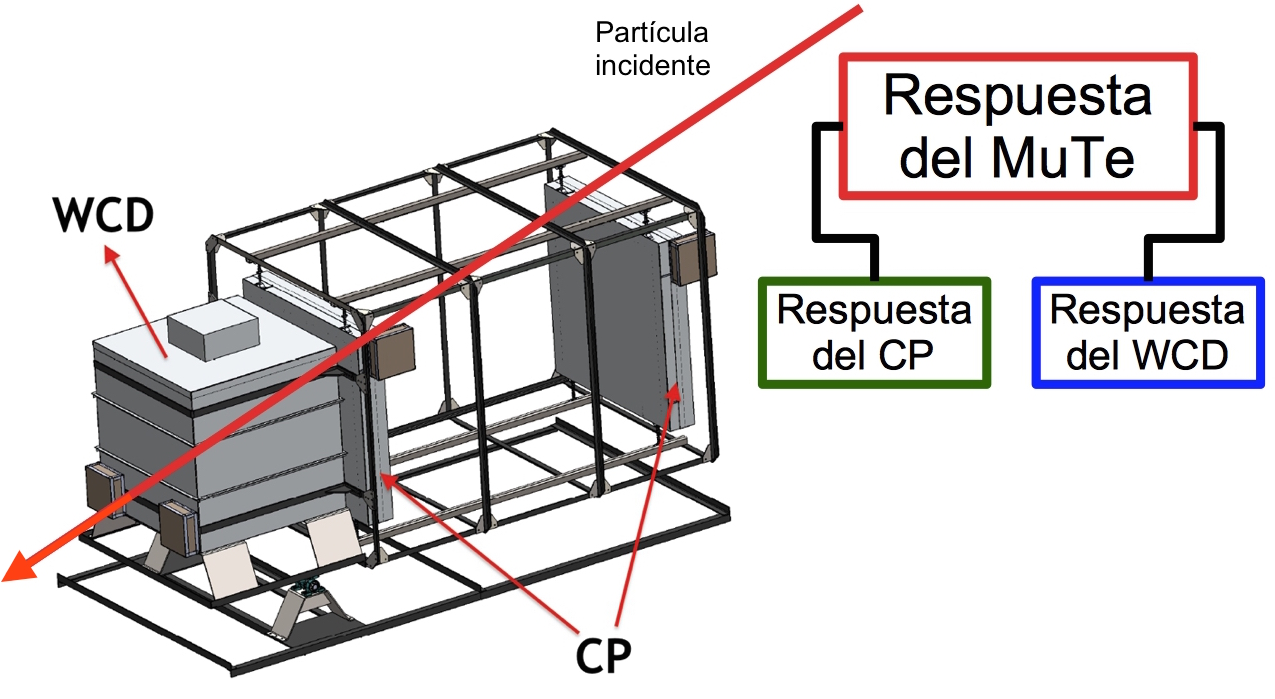
\includegraphics[scale=0.3]{mute.jpg}
\caption[Telescopio de Muones MuTe]{Telescopio de muones diseñado para la muongrafía de volcanes en Colombia. La respuesta del MuTe ante partículas cargadas se define en funci\'on de la respuesta del hodoscopio de centelladores plásticos y la respuesta del detector Cherenkov de agua.}\label{mute}
\end{figure}

El hodoscopio se emplea para estimar la dirección de las pat\'iculas cargadas provenientes del volcán. Como se observa en la figura \ref{pixels}, un pixel de detección se define como la intersección de la barra ubicada a lo largo del eje vertical, Y, con la barra ubicada en el eje horizontal, X, del panel. Existe una única dirección promedio dada por el pixel de la matriz frontal y el pixel de la matriz trasera. 
\begin{figure}[h!]
    \centering        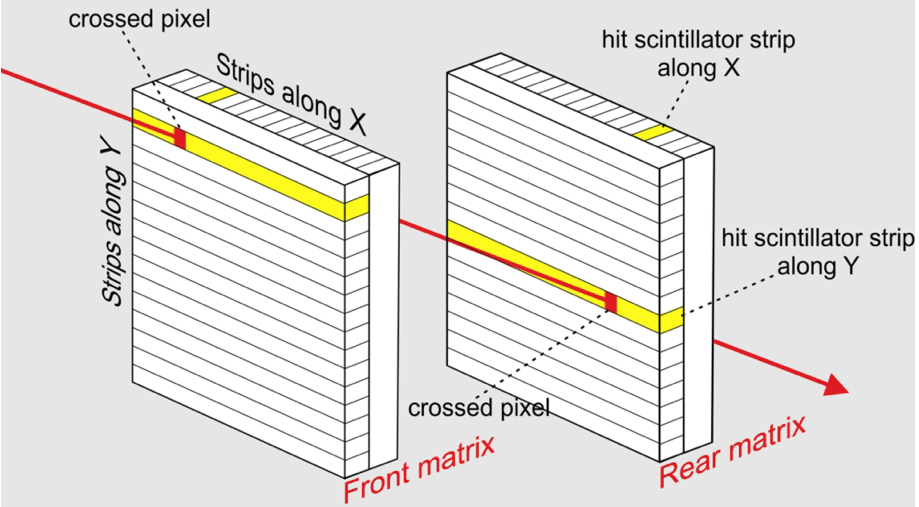
\includegraphics[scale=0.5]{pixels.png}
   \caption[Esquema de funcionamiento de un hodoscopio de muones con barras de centelleo]{Esquema de funcionamiento de un telescopio de muones con barras de centelleo: un muón golpea dos pares de barras X e Y en la matriz frontal y trasera, respectivamente, permitiendo estimar la dirección de la partícula (flecha roja) \cite{Carbone-etal2014}.}\label{pixels}
\end{figure}

Detrás del hodoscopio se ubica el detector Cherenkov de Agua (ver figura \ref{mute}), para identificar si la respuesta de la part\'icula incidente pertenece a la componente mu\'onica del flujo de secundarios. Además, esta configuraci\'on permite seleccionar s\'olo los eventos requeridos para realizar la muongraf\'ia, en este caso, aquellos muones que han atravesado el volc\'an ser\'an detectados en el MuTe en el siguiente orden:
\begin{enumerate}
\item Panel delantero del hodoscopio.
\item Panel trasero del hodoscopio.
\item WCD.
\end{enumerate}
La detecci\'on en cualquiera de los paneles se define como el registro de un número de fotoelectrones $N_\mathrm{FE}$ en un tiempo $t$, en el SiPM de dos centelladores (X e Y), mientras que el impacto en el WCD viene dado por el conteo de $N_\mathrm{FE}$ en el PMT, en un tiempo dado.

Antes de adquirir los datos con el MuTe es necesario realizar una calibración adecuada y para esto se debe determinar cómo responde el detector ante partículas cargadas. La presente investigación se basa en la estimación del número de fotoelectrones registrados al paso de partículas cargadas a trav\'es del hodoscopio (respuesta del CP), y del WCD del MuTe (respuesta del WCD en la figura \ref{mute}). Estos eventos se pueden simular con alto detalle utilizando la herramienta Geant4 \cite{Geant4} (para detalles consultar apéndice).

Para iniciar la técnica de la muongrafía en Colombia se estudiaron las condiciones geogr\'aficas de 12 volcanes, siendo el Cerro Machín el \'unico que cumple los siguientes criterios \cite{MuTeSites}:
\begin{itemize}
\item El ancho de la base del volcán es menor de 1500 m en el nivel de observación.
\item En los puntos de observación seleccionados la topografía que rodea el volcán no afecta las medidas, es decir, los muones que impactan el telescopio cruzan solamente el volcán.
\item Los sitios de observación son accesibles y seguros, con los recursos necesarios para instalar el detector MuTe. 
\item Los sitios de observación están fuera de riesgo debido a la actividad volcánica. 
\end{itemize}
\begin{figure}[h!]
    \centering
        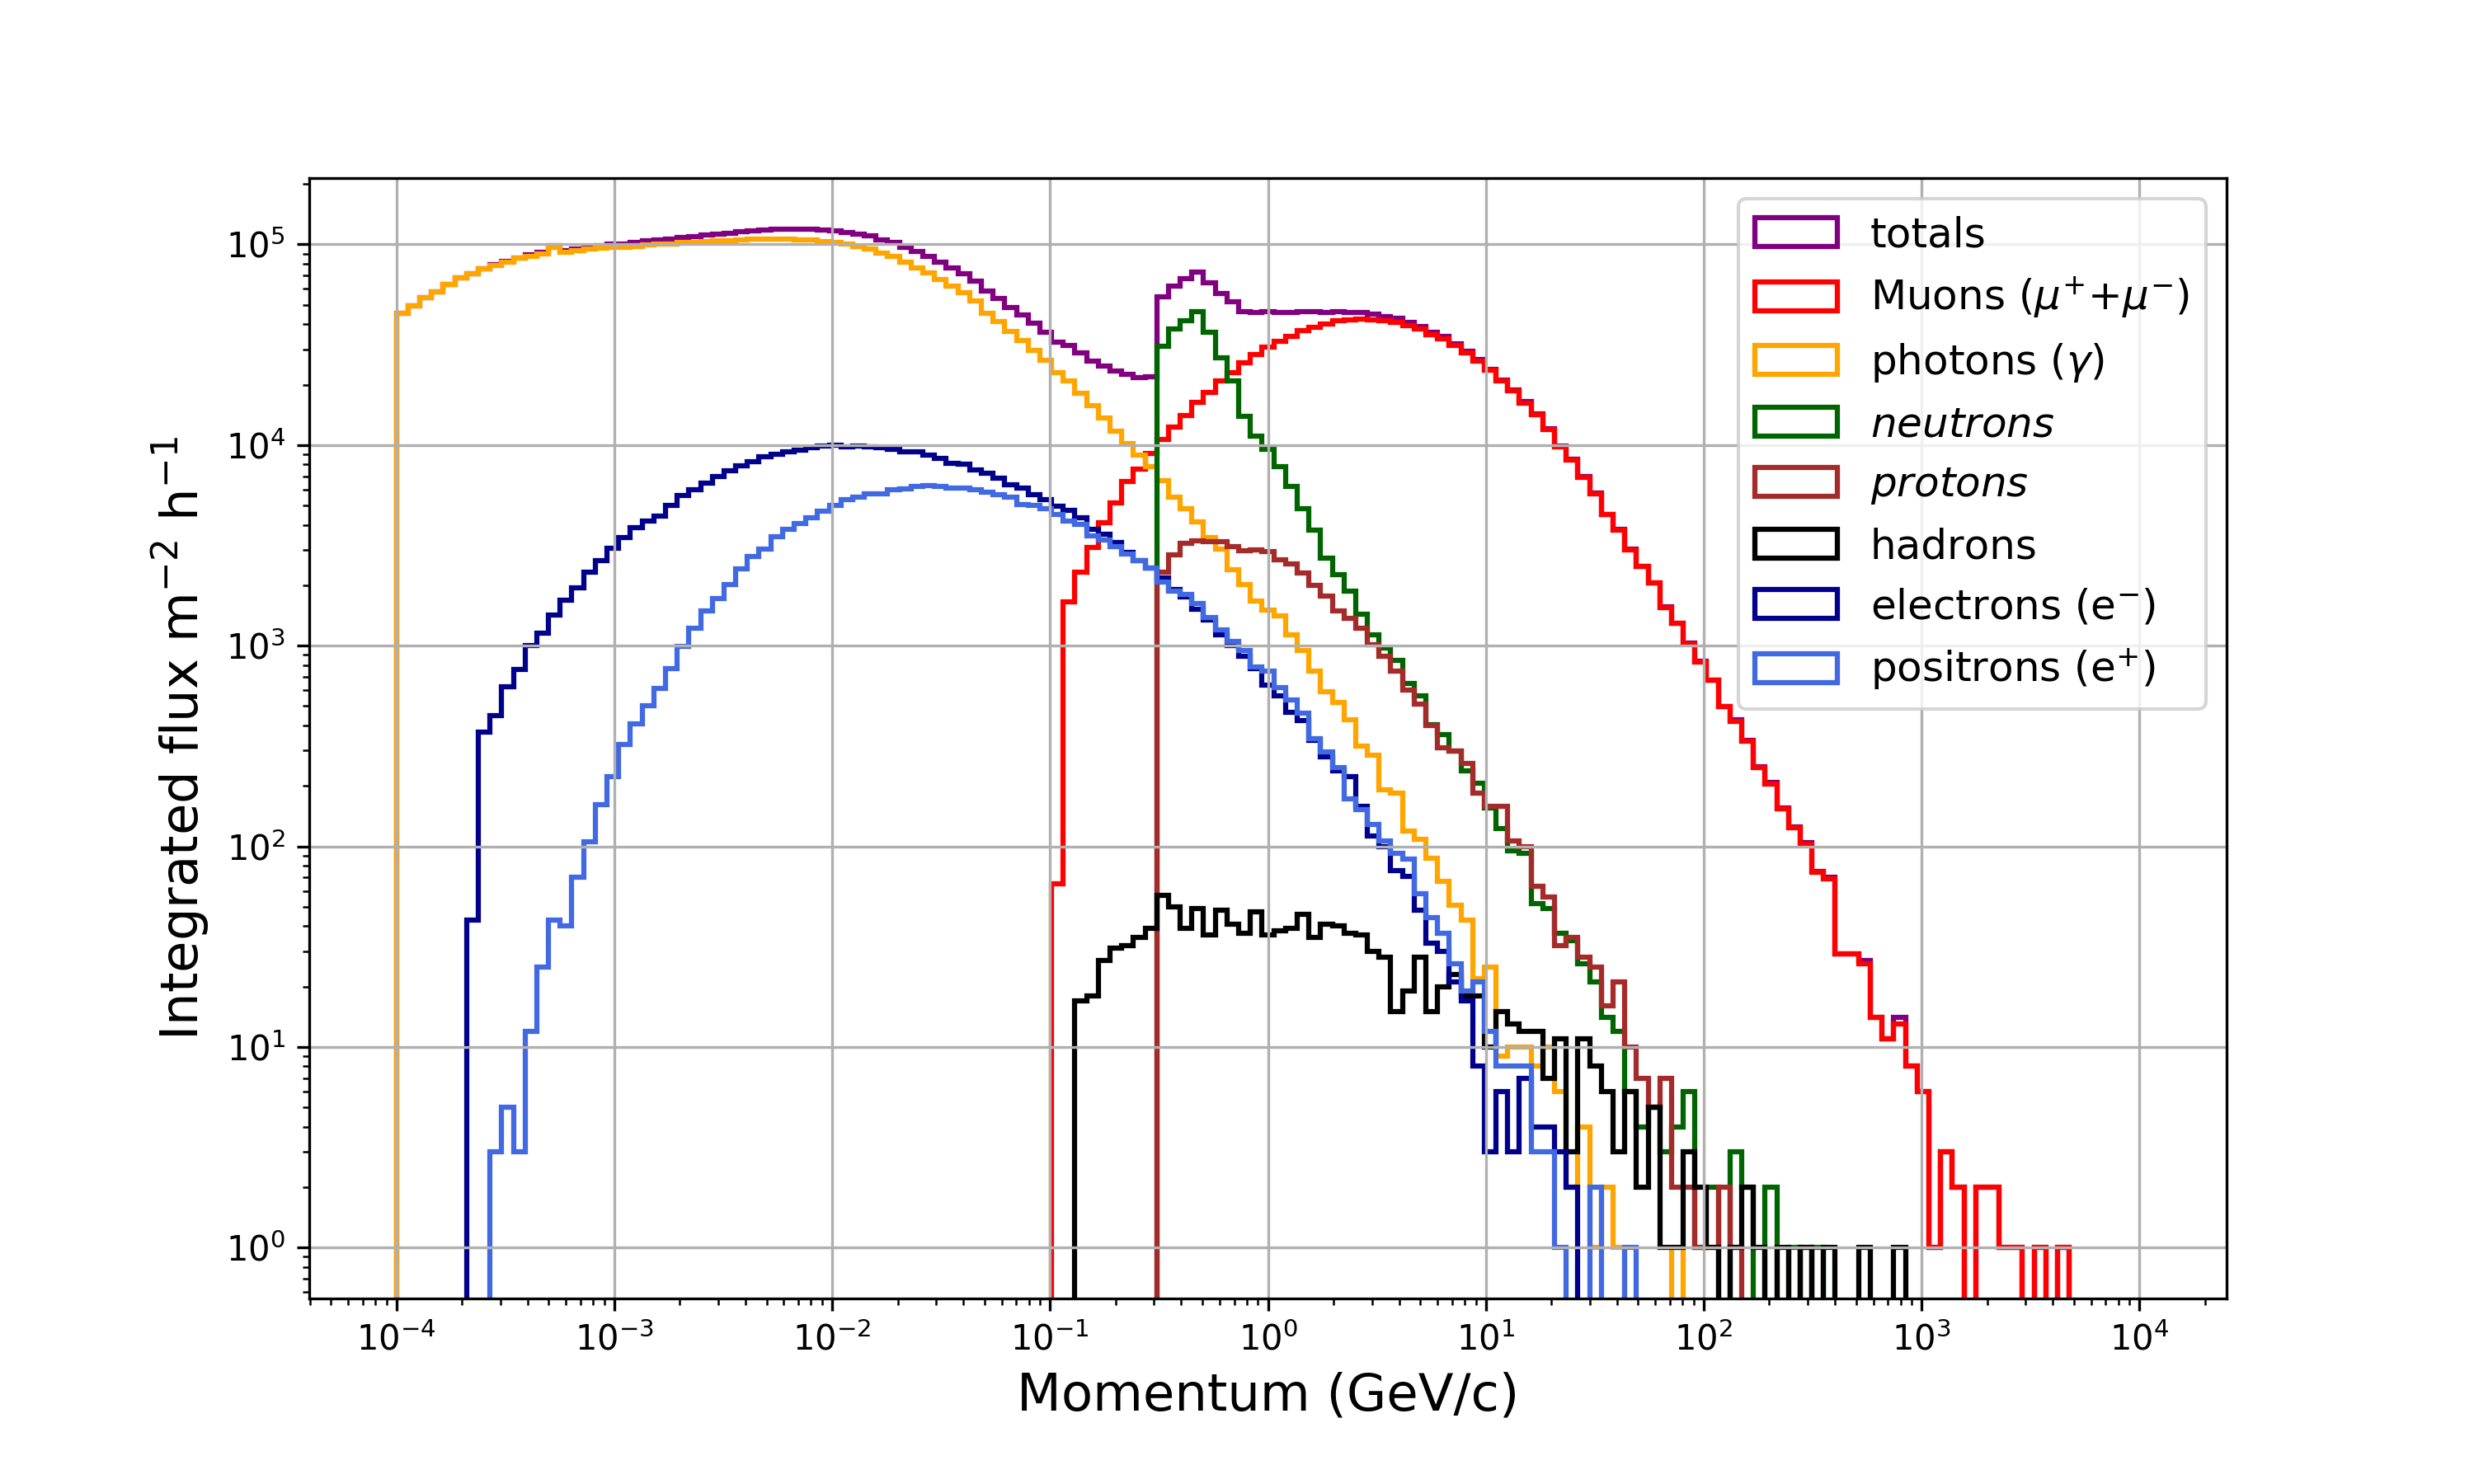
\includegraphics[scale=0.55]{countsenergies.png}
   \caption[Flujo integral de partículas secundarias a nivel del Volcán Cerro Machín]{Flujo integral de partículas secundarias a nivel del Volcán Cerro Machín (2750 m s.n.m.) \cite{MuTeSites}. Se observa que los muones más probables llegan con una energía alrededor de los 3 GeV, mientras que los electrones lo hacen con una energía de 20 MeV.}\label{flujo}
\end{figure}

Este volcán se encuentra a 2750 m s.n.m. con latitud de $4^{\circ}$29'23.08'' norte y longitud de $75^{\circ}$23'15.30'' oeste. A partir de estas coordenadas se puede estimar el flujo de partículas secundarias al que estará expuesto el detector MuTe. En la figura \ref{flujo} se muestra el flujo integral de partículas secundarias a nivel del Volcán Cerro Machín, corregido por campo geomagnético, obtenido en \cite{MuTeSites} a partir de simulaciones realizadas con MAGCOS y CORSIKA.

En los siguientes capítulos se muestran los resultados obtenidos de simular la respuesta del hodoscopio ante muones monoenergéticos y la respuesta del WCD ante muones y electrones monoenergéticos. Igualmente se detalla la respuesta del WCD ante el flujo de partículas secundarias a nivel del Volcán Cerro Machín dado por el gr\'afico \ref{flujo}. 

%%%%%%%%%%%%%%%%%%%%%%
%%%%% CHAPTER 3  %%%%%
%%%%%%%%%%%%%%%%%%%%%%

\chapter{Detector MuTe: El hodoscopio } \label{cap3}
El hodoscopio del MuTe está conformado por dos paneles que definen una matriz de detección de $30\times 30$ barras centelladoras cada uno. Esta configuración establece un total de 900 píxeles, dados por la intersección de una barra horizontal ($C_i$ para el panel delantero y $C_k$ para el trasero) y una barra vertical ($C_j$ o $C_l$, para el panel frontal o trasero, respectivamente), como se muestra en la figura \ref{sistema_coo}. Al definir los píxeles de detección del panel frontal como $P^{F}_{i,j}$ y los del panel trasero como $P^{T}_{k,l}$, se puede determinar la trayectoria de la partícula a partir de las coordenadas $Y(i,k)$ y $Z(j,l)$, con una distancia constante entre los paneles, $X = d$. Todo par de píxeles $\{P^{F}_{i,j},\, P^{T}_{k,l}\}$ con la misma posición relativa $\{m=k-i,\, n=l-j\}$, comparten la misma dirección promedio $\mathbf{r}_{m,n}$, dada por
\begin{equation}
\mathbf{r}_{m,n} = \frac{-d \hat{x} +m\hat{y} +n \hat{z}}{r},
\end{equation}
donde $r=\sqrt{d^2+m^2+n^2}$. 

Por ejemplo, en la figura \ref{sistema_coo} se tiene que una part\'icula (flecha naranja) que ha impactado en el pixel del panel frontal $P^{F}_{30,30}$, y luego en el pixel del panel trasero $P^{T}_{30,30}$, ha llegado completamente horizontal, con una direcci\'on dada por 
\begin{equation}
\mathbf{r}_{0,0} =\frac{-d\, \hat{x} +(30-30)\hat{y} +(30-30) \hat{z}}{d}=-\hat{x}.
\end{equation}

\begin{figure}[h!]
    \centering       
    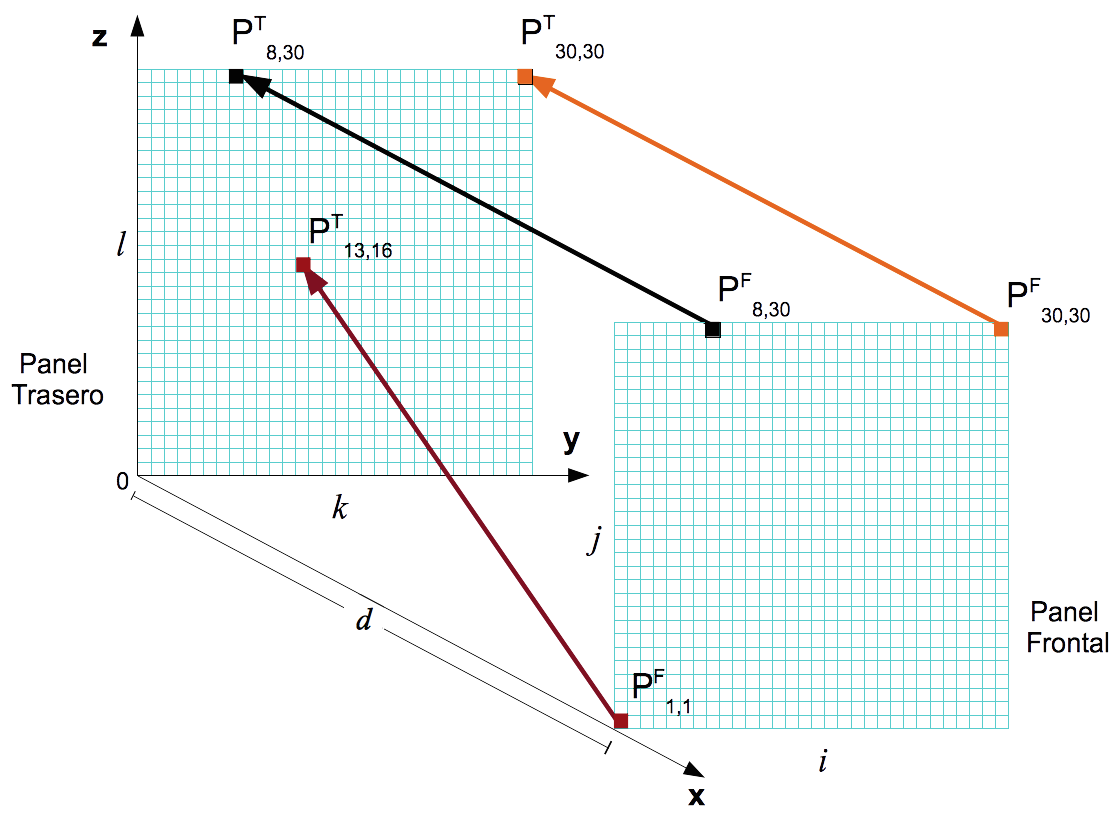
\includegraphics[scale=0.5]{sistema_coo.png}
    
   \caption[Sistema de coordenadas del hodoscopio del MuTe]{Sistema de coordenadas del hodoscopio del MuTe, en términos de los pixeles de detección de los paneles de centelladores plásticos. El panel frontal está conformado por los pixeles $P^{F}_{i,j}$, mientras que el panel trasero contiene los pixeles $P^{T}_{k,l}$. La señal producida al paso de un muón en el SiPM del centellador $C_i$ y del centellador $C_j$, en el panel delantero, y $C_k$ y $C_l$ en el panel trasero, definen la dirección de arribo de la partícula, $\mathbf{r}_{m,n}$. Las flechas representan tres ejemplos hipotéticos de trayectorias recorridas por muones y los pixeles activados en cada caso.}\label{sistema_coo}
\end{figure}

De esta manera, el número de muones $N_{\mu}$ detectados por el hodoscopio para una dirección $\mathbf{r}_{m,n}$, viene dado por
\begin{equation}
\label{ecNumero}
N_{\mu}(\mathbf{r}_{m,n}, \, \Delta \tau)= I_{\mu}(\mathbf{r}_{m,n}) \times \Delta \tau \times T(\mathbf{r}_{m,n}),
\end{equation}
donde $I_{\mu}$ es el flujo integral de muones dado en cm$^{-2}$ sr$^{-1}$ s$^{-1}$,  $\Delta \tau$ es el tiempo de exposici\'on del instrumento en el sitio de observaci\'on, y $T$ es la aceptancia del telescopio expresada en cm$^2$ sr \cite{lesparre-etal2012-gim}. Detalles sobre el cálculo de $\Delta \tau$ y $T$ del MuTe, para una distancia $d=200$cm, se encuentran en \cite{MuTeSites}.

Para estudiar la respuesta del hodoscopio se debe conocer primero la respuesta del detector de centelleo. A continuaci\'on se muestran las características y propiedades físicas que se tomaron en cuenta para la simulación de los centelladores en el código de Geant4.


%%%%%%%%%%%%%%%%%%%%%%%%%%%%%%%
%%%%%%%%%   Section   %%%%%%%%%
%%%%%%%%%%%%%%%%%%%%%%%%%%%%%%%

\section{Detector de Centelleo}
\begin{figure}[h!]
    \centering       
    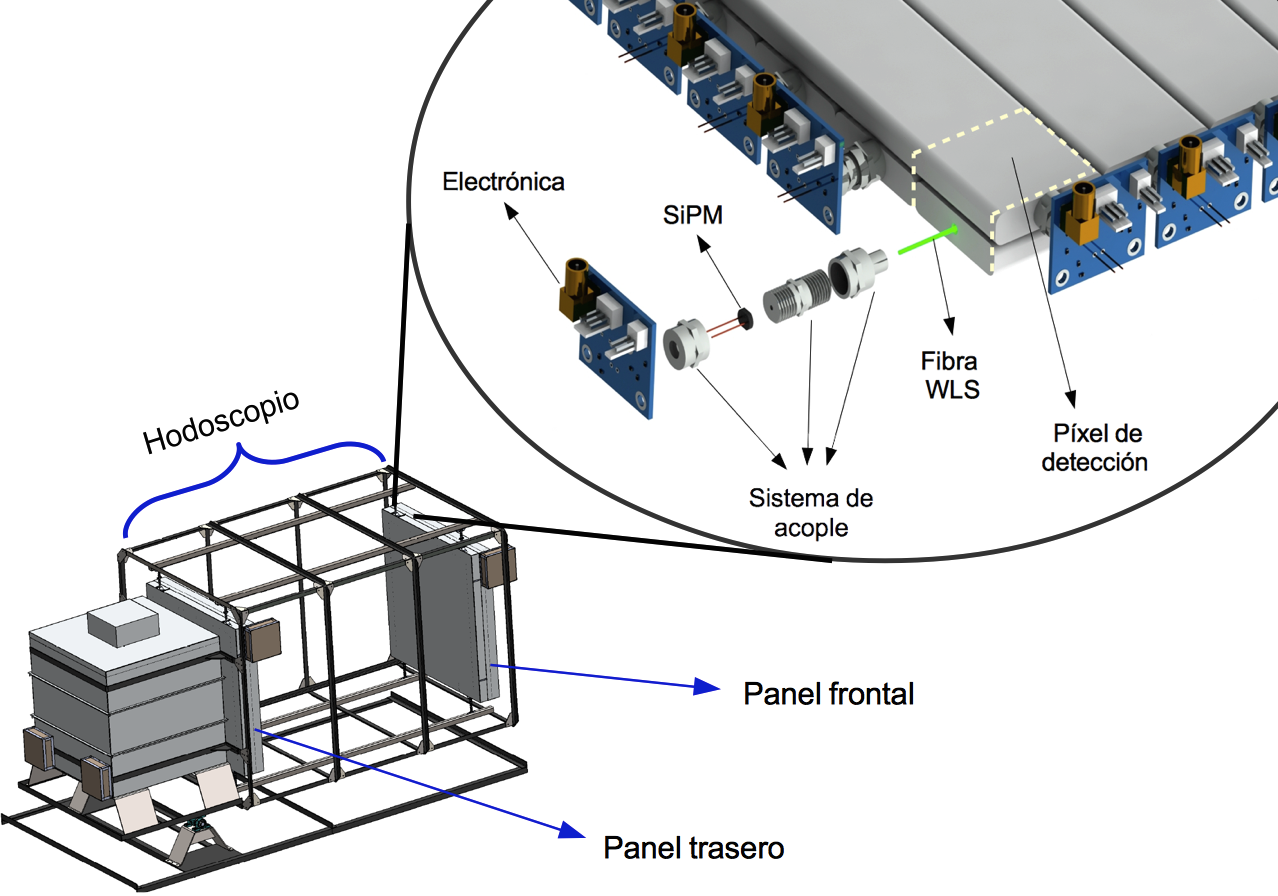
\includegraphics[scale=0.5]{hodoscopio.png}
    % \includegraphics[scale=0.5]{panel_desc.png}
   \caption[Detalle de la configuración de un panel del hodoscopio del MuTe]{Detalle de la configuración de un panel del hodoscopio del MuTe. Los pixeles se delimitan por la intersecci\'on de un centellador orientado verticalmente sobre otro centellador orientado horizontalmente, definiendo una superficie de detecci\'on de 4$\times$4 cm$^{2}$. Por ejemplo, el pixel $P^{F}_{1,1}$ se delimita por la línea amarilla. Además, se muestran los componentes del detector de centelleo: la barra centelladora con la fibra WLS en su interior que se acopla al SiPM y éste a su vez a la electrónica, a través de un sistema mecánico.}\label{panel_desc}
\end{figure}
%%%%%%%%%%%%%%%%%%%%%%%%%%%%%%%
%%%%%%%%% Subsection  %%%%%%%%%
%%%%%%%%%%%%%%%%%%%%%%%%%%%%%%%
\subsection{Barra Centelladora}
Las barras centelladoras del MuTe tienen 120 cm de largo, 4 cm de ancho y 1 cm de espesor, formando p\'ixeles con una superficie de detecci\'on de 4 cm $\times$ 4 cm, como se señala en la figura \ref{panel_desc}. Están hechas de poliestireno (Dow Styron 663) dopado con 1\% de 2,5-diphenyloxazole (PPO) y $0.03\%$ de 1,4-bis(5-Phenyloxazole-2-yl) benceno (POPOP). Con esta composición se tiene un pico de emisión centrado en una longitud de onda de $\sim 420 $ nm. Además están revestidas con poliestileno claro con $\text{TiO}_{2}$ en una concentración del $15\%$  \cite{pla-etal2003}. El campo de luz producido por estos centelladores es bastante uniforme con variaciones de $\pm 5 \%$, y tienen una longitud de atenuación de $\sim 55\pm 5$ mm para la componente rápida (proceso de centelleo) y de 24 cm para la componente lenta (proceso de fosforescencia) \cite{amiga-etal2016}.

A lo largo de las barras se tiene una perforación centrada de $\sim 3$ mm de diámetro, donde se sitúa la fibra óptica WLS que absorbe los fotones producidos en el centellador para reemitirlos con una energía menor y transportarlos hasta el SiPM. 

Para la simulaci\'on se utilizaron barras de poliestireno revestidas de poliestileno claro con $\text{TiO}_{2}$, con una longitud de atenuación de fotones de 5.5 cm.

\subsection{Fibra} 
Las fibras del detector son las correspondientes a la referencia BCF99-29AMC de Saint-Gobain, cuyo diámetro es de 1 mm. Estas fibras son de multirevestimiento con un interior de PMMA (Polimetilmetacrilato, $C_5H_8O_2$) con 1.2 g/cm$^3$ de densidad y un índice de refracción ($n_{f}$) de 1.6. Están recubiertas con una primera capa de acrílico ($n_{c1} =$ 1.49) seguida de otra capa de fluor-acrílico ($n_{c2} = $1.42). La diferencia en estos \'indices de refracci\'on produce una reflexión tal que los fotones reemitidos en la fibra, viajen a lo largo de ésta como se ve en la figura \ref{fiber_cladding}. La fibra tiene una longitud de atenuación para los fotones de más de 3.5 m, un tiempo de decaimiento de 2.7 ns y un máximo de absorción y emisión de luz centrado en 410 nm y 485 nm, respectivamente \cite{saint-gobain-fiber}. Las fibras BCF99-29AMC tienen los mismos dopantes que la referencia estándar BCF-92\footnote{\url{https://www.crystals.saint-gobain.com/products/scintillating-fiber}} de los catálogos de Saint Gobain, pero con el doble de concentración. El sistema multi-revestimiento aumenta la señal en un 60\% comparado con las de revestimiento sencillo \cite{amiga-etal2016}. 

\begin{figure}[h!]
    \centering        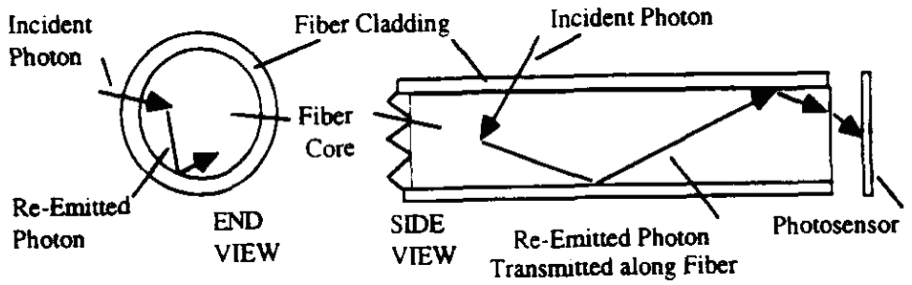
\includegraphics[scale=0.5]{fiber_cladding.png}
   \caption[Esquema de la absorción y reemisión de luz a través de una fibra óptica]{Esquema de la absorción y reemisión de luz a través de una fibra óptica que cambia la longitud de onda de los fotones (WLS) \cite{Worstell-etal1994}. A la derecha se observa el corte longitudinal de la fibra y a la izquierda el corte transversal. El revestimiento evita que los fotones reemitidos en el n\'ucleo de la fibra salgan de este volumen.}\label{fiber_cladding}
\end{figure}


En la simulaci\'on realizada en Geant4, la fibra consta de un cilindro de PMMA recubierto por los dos revestimientos descritos, como se muestra en la figura \ref{perfil_sipm}. En uno de los extremos se acopla el SiPM y en el otro se define una superficie óptica que absorbe los fotones que van en dirección contraria al SiPM. 

\begin{figure}[h!]
    \centering        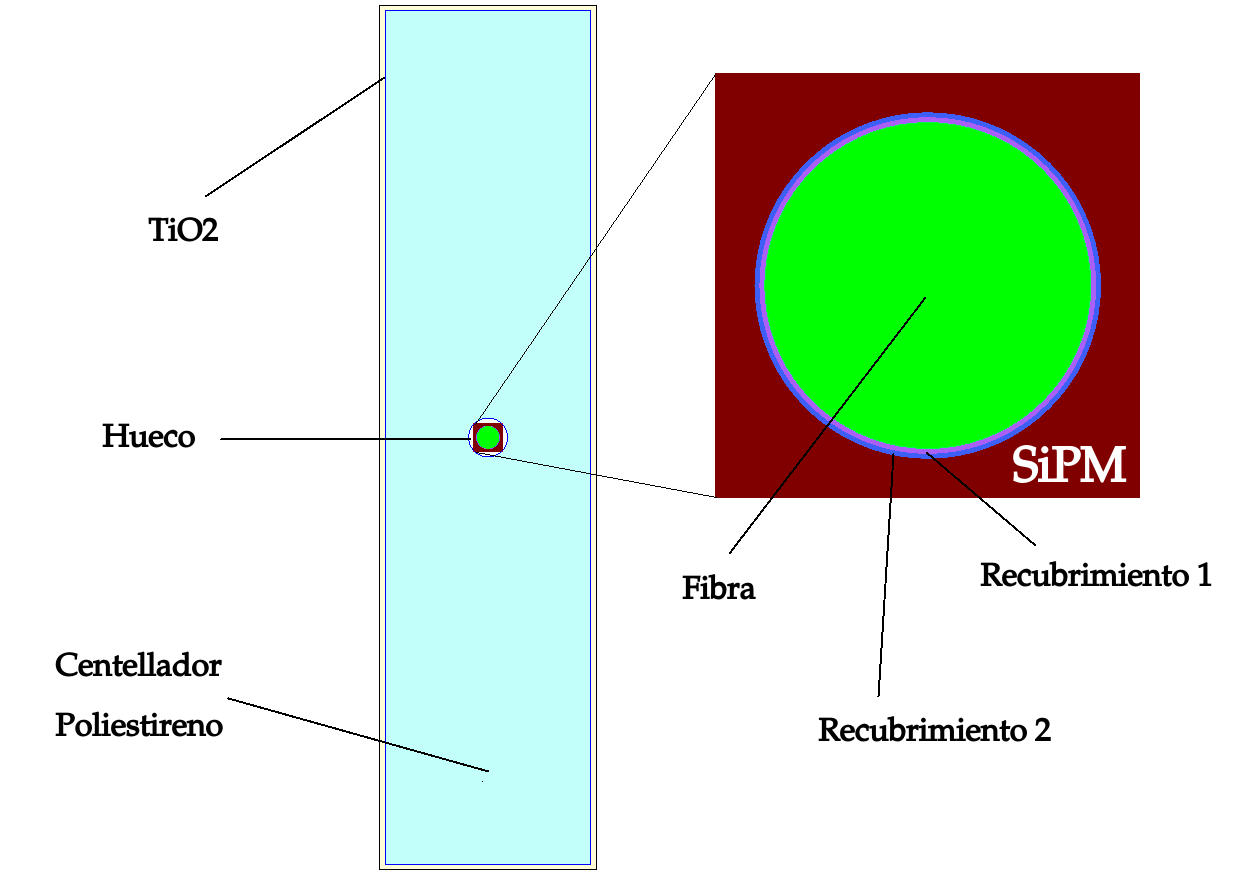
\includegraphics[scale=0.35]{perfil_sipm.png}
   \caption[Perfil del detector de centelleo simulado en GEANT4]{Perfil del detector de centelleo simulado en Geant4, conformado por la barra centelladora de poliestireno recubierta de poliestileno claro con $\text{TiO}_{2}$, la fibra WLS (verde) recubierta con acrílico (morado) y fluor-acrílico (azul), y el SiPM pegado en un extremo de la fibra para detectar los fotones.}\label{perfil_sipm}
\end{figure}

\subsection{Fotomultiplicador de Silicio}
Son dispositivos fotosensibles necesarios para registrar los fotones que viajan por la fibra óptica. Los SiPM son dispositivos opto-semiconductores compuestos por un arreglo de foto-diodos (píxeles) en avalancha, que conforman una matriz de detección capaz de registrar fotones individuales \cite{HamamatsuSipmMeasu}. Cuando un fotón hace contacto con uno de los píxeles del SiPM, éste excita un electrón de la banda de conducción y crea un par electrón-hueco que se moverá de acuerdo a la orientación del campo eléctrico de polarización del dispositivo.

Para la simulación del SiPM\footnote{\url{http://www.hamamatsu.com/resources/pdf/ssd/s13360_series_kapd1052e.pdf}} se ha optado por definir una superficie cuadrada de 1.3 mm de lado, ubicado en uno de los extremos de la fibra (ver superficie cuadrada roja de la figura \ref{perfil_sipm}). Además se ha introducido su eficiencia cuántica en el código, de modo que un fotón que alcance esta superficie será detectado o absorbido según la probabilidad de detección correspondiente a su longitud de onda. La eficiencia cu\'antica del SiPM del MuTe se muestra en la figura \ref{QESIPM}, donde se observa una eficiencia máxima del 25\% para detectar fotones con $\lambda = 450$ nm.

\begin{figure}[h!]
    \centering
        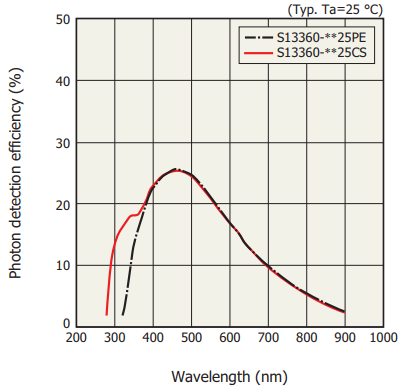
\includegraphics[scale=0.7]{QESIPM.png}
   \caption[Eficiencia cuántica del SiPM S13360-1325PE de Hamamatsu]{Eficiencia cuántica del SiPM S13360-1325PE de Hamamatsu, con un máximo de detección de fotones para una longitud de onda alrededor de 450 nm. A partir de esta curva se establece en el c\'odigo de Geant4 la probabilidad de detecci\'on de los fotones seg\'un su longitud de onda (Figura tomada de \url{http://www.hamamatsu.com/resources/pdf/ssd/s13360_series_kapd1052e.pdf}).}\label{QESIPM}
\end{figure}

%%%%%%%%%%%%%%%%%%%%%%%%%%%%%%%
%%%%%%%%%   Section   %%%%%%%%%
%%%%%%%%%%%%%%%%%%%%%%%%%%%%%%%

\section{Respuesta del Detector de 
Centelleo}
La respuesta del centellador depende del poder de frenado de cada una de las partículas cargadas que impactan. En este caso se tiene que el poder de frenado de los muones en el poliestireno es de 2 MeV cm$^2/$g, en un amplio rango de energías (ver figura \ref{stopping_mu_scint}). Para los electrones ocurre lo mismo en un rango menor de energía, aproximadamente entre 0.5 MeV y 20 MeV (ver figura \ref{stopping_e_scint}). Por lo tanto, se puede considerar que la respuesta del centellador de poliestireno es similar al paso de muones y electrones de energ\'ias t\'ipicas, es decir, de muones de alrededor de 3 GeV y de electrones con energ\'ias alrededor de los 20 MeV. A continuaci\'on se muestran los resultados de simular la respuesta del detector de centelleo ante muones monoenerg\'eticos.  
\begin{figure}[h!]
    \centering        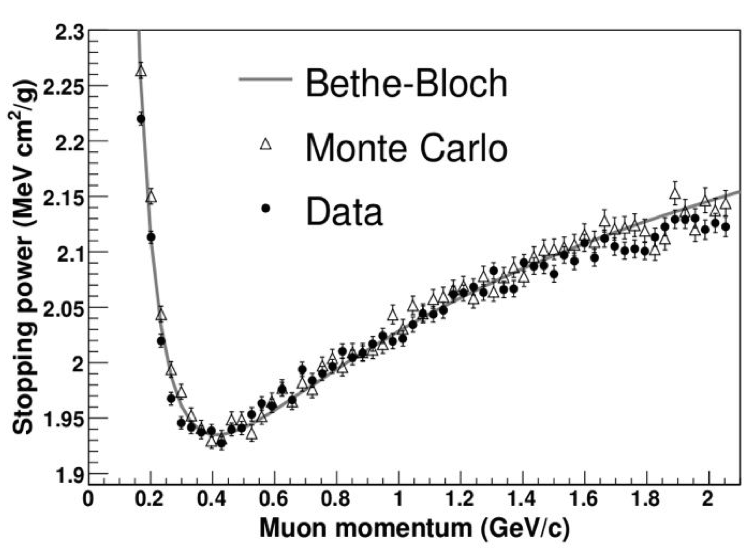
\includegraphics[scale=0.6]{stopping_mu_scint.png}
\caption[Poder de frenado para muones en poliestireno]{Poder de frenado para muones en poliestireno \cite{Gonzalez-maestrando2012}. Se puede observar que para este rango de energ\'ias el poder de frenado est\'a alrededor de los 2 MeV cm$^2/$g aproximadamente.}\label{stopping_mu_scint}
\end{figure}
\begin{figure}[h!]
    \centering        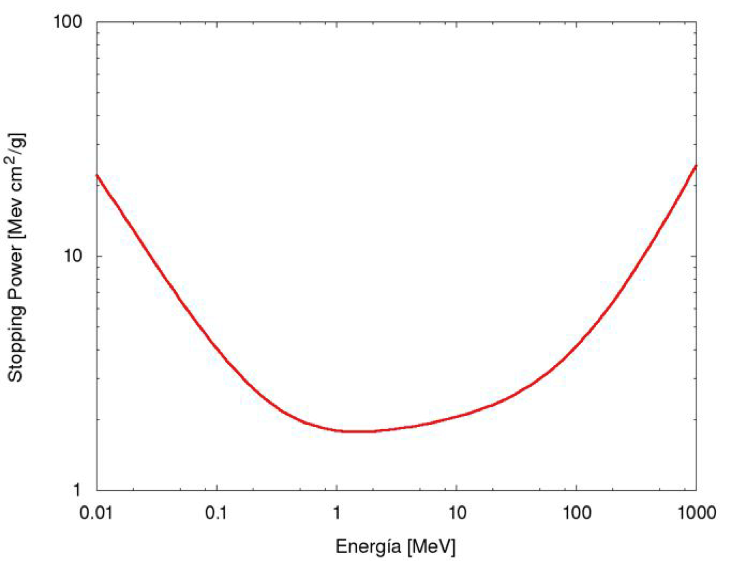
\includegraphics[scale=0.6]{stopping_e_scint.png}
\caption[Poder de frenado para electrones en poliestireno]{Poder de frenado para electrones en poliestireno \cite{Gonzalez-maestrando2012}. Los electrones de energ\'ia t\'ipica (decenas de MeV) tienen un poder de frenado alrededor de los 2 MeV cm$^2/$g.}\label{stopping_e_scint}
\end{figure}
\subsection{Pulso característico de la señal de un muón de 3 GeV}
\begin{figure}[h!]
    \centering
     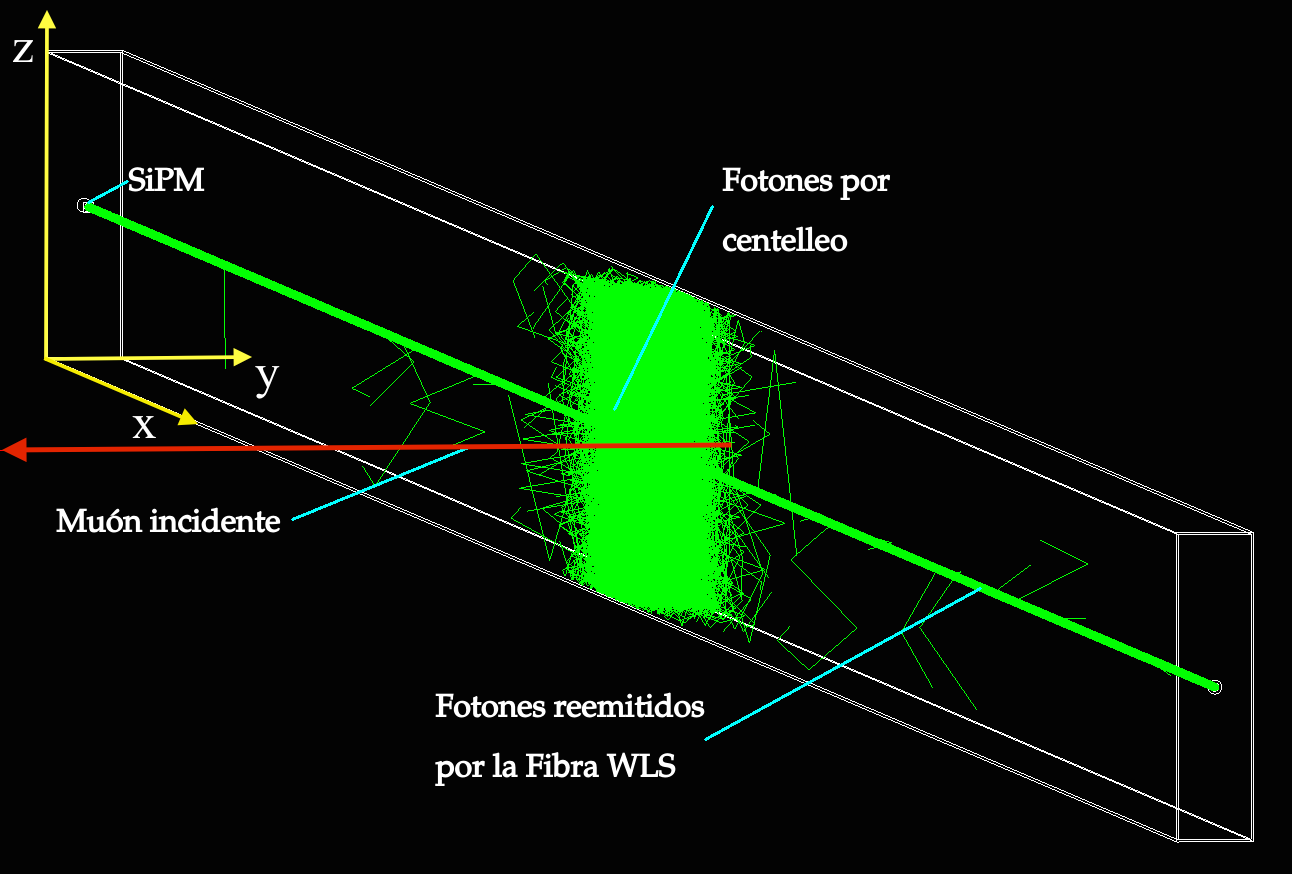
\includegraphics[scale=0.45]{11.png}
   \caption[Cadena de sucesos para la detección de un muón de 3 GeV que incide horizontalmente sobre un detector de centelleo]{Cadena de sucesos simulada en Geant4 para la detección de un muón de 3 GeV que incide horizontalmente (en direcci\'on $-\hat{y}$) sobre un detector de centelleo, a 62 cm del SiPM (en el eje $x$). Cuando el muón atraviesa la barra se produce un número de fotones por centelleo, con una atenuaci\'on media de 5.5 cm en el poliestireno. Parte de estos fotones son absorbidos por la fibra y reemitidos con una energía menor en su interior, para viajar hacia el SiPM o hacia el extremo opuesto. Los fotones que llegan al SiPM pueden ser detectados según la eficiencia cu\'antica de \'este, mientras que los que viajan al otro extremo son absorbidos por el medio.}\label{barra_muon}
\end{figure}

La detección de un muón genera un pulso característico dado en términos del número de fotoelectrones producidos en el SiPM, en un tiempo $t$. Para obtenerlo se simuló en Geant4 el impacto de 10000 muones de 3 GeV que ingresan perpendicularmente a la barra. La posici\'on inicial de la part\'icula se escoge de tal manera que impacte en el centro de los pixeles de detecci\'on definidos para los paneles del hodoscopio, por ejemplo, para que el mu\'on impacte en el centro del primer pixel, $P_{1,1}$, se define su posici\'on inicial a 2 cm del SiPM. De esta manera, la posici\'on inicial del mu\'on para impactar en el punto medio de cada pixel, se define como 
\begin{equation}
\label{posiciones}
x_p = (2 + 4n)\mathrm{cm} \,\,\,\,\,\,\,\,\,\, y_p = 1\mathrm{cm}  \,\,\,\,\,\,\,\,\,\, z_p = 2\mathrm{cm},
\end{equation}
a partir del sistema de referencia definido en la figura \ref{barra_muon}, con $y_p$ y $z_p$ constantes, y $p=0,1,2,...,29$. 

El pulso promedio resultante del impacto de estos muones sobre la barra se observa en la figura \ref{Pulsos_barra}. En el primer caso, cuando el mu\'on ha ingresado a 2 cm del SiPM (figura \ref{a2cm_pulso}), se puede notar que el 40\% de los fotoelectrones se producen en los primeros 10 ns, mientras que en el segundo caso s\'olo se produce el 12\% (figura \ref{a118cm_pulso}).  
\begin{figure}[h!]
    \centering
    \begin{subfigure}{0.44\textwidth}
        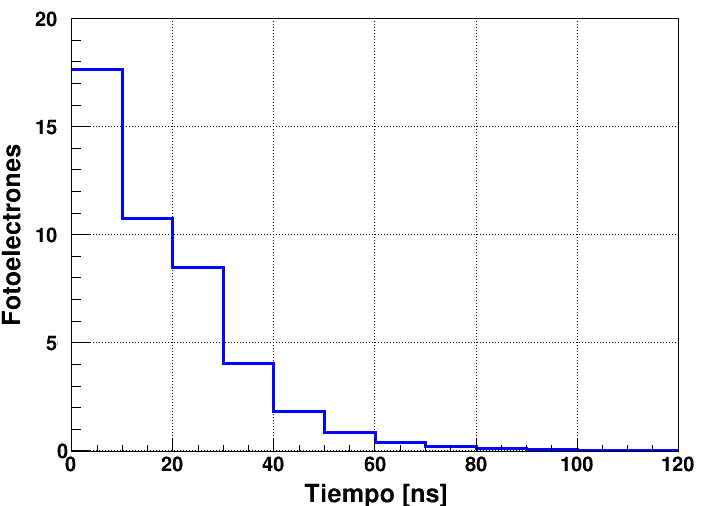
\includegraphics[width=\textwidth]{a2cm_pulso.png}
        \caption{}
        \label{a2cm_pulso}
    \end{subfigure}
    \begin{subfigure}{0.5\textwidth}
        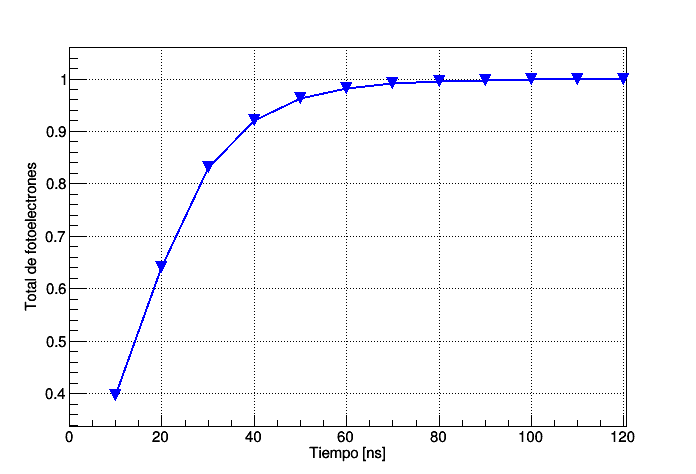
\includegraphics[width=\textwidth]{2cmcum.png}
        \caption{}
        \label{2cmcum}
    \end{subfigure}
    \begin{subfigure}{0.44\textwidth}
        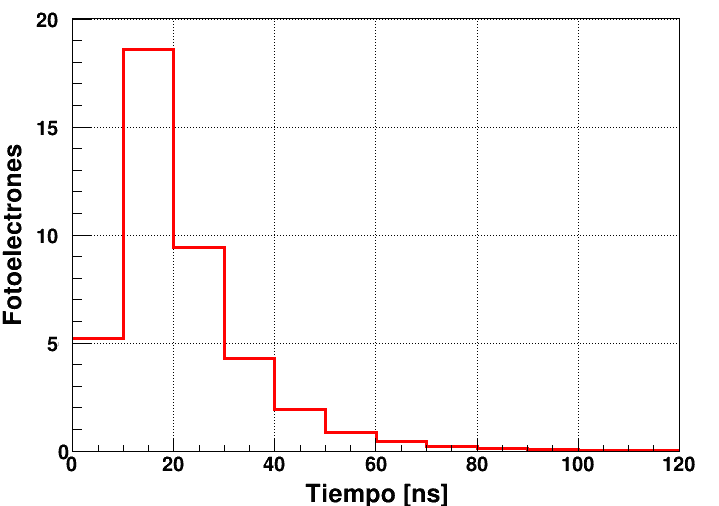
\includegraphics[width=\textwidth]{a118cm_pulso.png}
        \caption{}
        \label{a118cm_pulso}
    \end{subfigure}
    \begin{subfigure}{0.5\textwidth}
        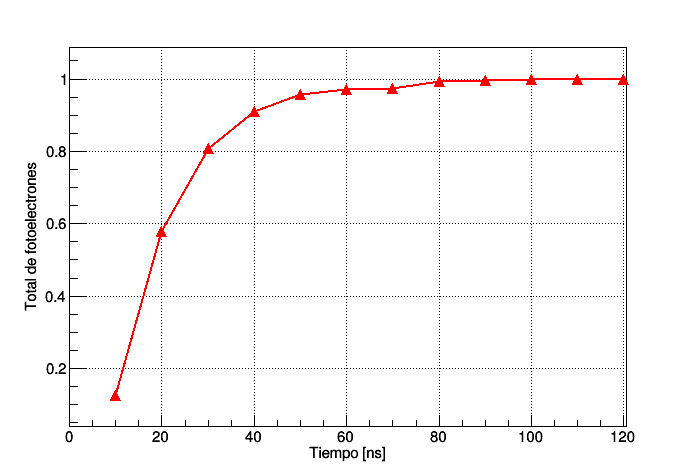
\includegraphics[width=\textwidth]{118cmcum.png}
        \caption{}
        \label{118cmcum}
    \end{subfigure}
    \caption[Pulso medio correspondiente a un muón de 3 GeV en el detector de centelleo]{Pulso medio correspondiente a la respuesta del detector de centelleo ante el impacto de un muón de 3 GeV que ingresa a 2 cm de distancia al SiPM (a) y a 118 cm (c). En la figura (b) se puede observar que para el caso (a) se acumula el 40\% del total de los fotoelectrones del pulso en los primeros 10 ns, mientras que en el caso (c) sólo se acumula el 12\% en la misma ventana temporal (d).}\label{Pulsos_barra}
\end{figure}

Estos dos casos representan los extremos de la barra centelladora y el número total de fotoelectrones producidos en cada uno presentan una leve diferencia. Teniendo entonces que a 2 cm del SiPM se producen en promedio 40 fotoelectrones y a 118 cm se producen 37, como se muestra en los gráficos \ref{fotoelec_2cm} y \ref{fotoelec_118cm}, respectivamente. Esta diferencia se asocia a la atenuación de los fotones que viajan por la fibra y para obtener la curva característica, se simuló la respuesta del detector de centelleo en las 30 posiciones dadas por los puntos definidos en las ecuaciones \ref{posiciones}. Los resultados se detallan en la sección (\ref{atenuacion_seccion}).
\begin{figure}[h!]
    \centering
    \begin{subfigure}{0.6\textwidth}
        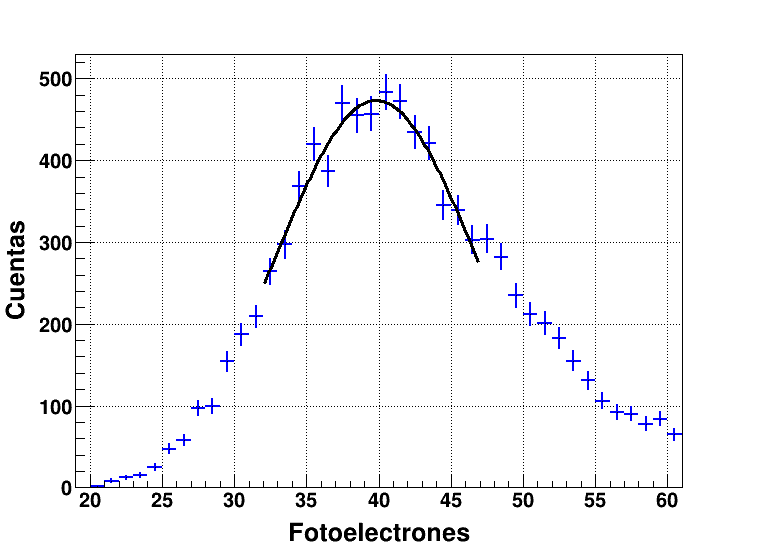
\includegraphics[width=\textwidth]{fotoelec_2cm.png}
        \caption{}
        \label{fotoelec_2cm}
    \end{subfigure}
    \begin{subfigure}{0.6\textwidth}
        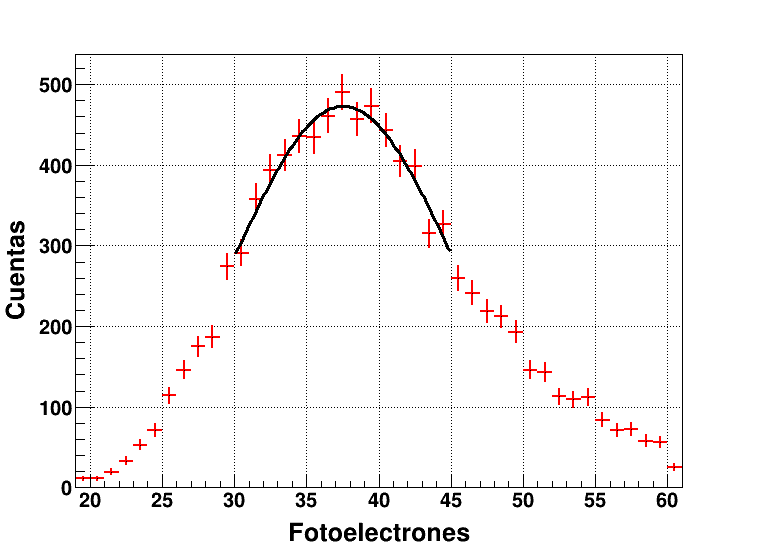
\includegraphics[width=\textwidth]{fotoelec_118cm.png}
        \caption{}
        \label{fotoelec_118cm}
    \end{subfigure}
    \caption[Número medio de fotoelectrones producidos por el impacto de un muón sobre la barra centelladora]{Número medio de fotoelectrones producidos por el impacto de un muón de 3 GeV sobre la barra centelladora, a 2 cm del SiPM (a) y 118 cm del SiPM (b). (a) El pico está centrado en 40 fotoelectrones mientras que en (b) se centra en 37, presentando una diferencia de 3 fotoelectrones entre ambos extremos del centellador.}\label{fotoelect_barra_dif}
\end{figure}

\subsection{Atenuación del número de fotoelectrones}\label{atenuacion_seccion}
La atenuación de la señal en el detector de centelleo del MuTe, fue obtenida a través de medidas experimentales, dando como resultado un 11\% de diferencia entre el pico resultante de la señal de 10000 eventos a 2 cm del SiPM, y el pico correspondiente a la señal promedio de 10000 impactos a 118 cm del SiPM \cite{CalderonArdila2018}. Para comparar estos resultados se realizaron una serie de simulaciones, donde el muón de 3 GeV incide sobre la barra centelladora en los distintos puntos descritos en \ref{posiciones}. 

Para el primer pixel se obtuvo en promedio un total de 40 fotoelectrones, al paso de 10000 muones. Esta cantidad va decayendo conforme el impacto del muón se aleja del SiPM, como se muestra en la figura \ref{atenuacion_barra}. Típicamente la atenuación de fotones en estas fibras presenta un comportamiento exponencial \cite{Gonzalez-maestrando2012}, en este caso se obtuvo una función de ajuste para los datos, $F(x)$, con la siguiente forma
\begin{equation}
F(x)= \text{0.468} \exp(\text{-0.003}(2-x))+\text{0.531} \exp(\text{0.005}(2-x)),
\end{equation}
donde $x$ representa la posición de impacto del muón respecto al SiPM.
\begin{figure}[h!]
    \centering
        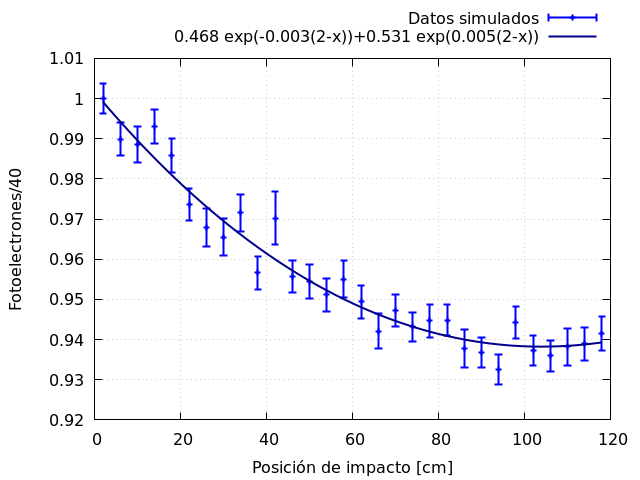
\includegraphics[scale=0.55]{atenuacion_barra_2.png}
   \caption[Atenuación del número de fotoelectrones respecto a la posición de impacto del muón en la barra]{Atenuación del número de fotoelectrones respecto a la posición de impacto del muón en la barra. A 2 cm del SiPM se tienen 40 fotoelectrones en promedio y a 118 cm del SiPM se tienen 37. La atenuaci\'on de fotones en el extremo opuesto al SiPM es aproximadamente del 7\% respecto a la posici\'on m\'as cercana a \'este.}\label{atenuacion_barra}
\end{figure}

\subsection{Importancia de la ubicación del SiPM}
Como se ha descrito, el SiPM es el dispositivo necesario para detectar aquellos fotones que viajan por la fibra. Para evaluar las diferencias entre un acople ideal y uno deficiente, se simuló la respuesta del detector de centelleo ante 10000 muones de 3 GeV (a 2 cm del SiPM) teniendo en cuenta dos casos:

\begin{enumerate}
\item SiPM ubicado justo al extremo de la fibra.
\item Distancia entre el SiPM y la fibra de 1.15 mm.
\end{enumerate}

El primer caso se escogió para realizar todas las simulaciones respecto a la respuesta del detector de centelleo, debido a que es la referencia ideal del sistema. En la figura \ref{perdida} se puede observar este caso en la parte superior, donde el SiPM recoge todos los fotones que han llegado al final de la fibra. En la parte inferior de la misma figura, se tiene el segundo caso y se observa que gran parte de los fotones que llegan al extremo de la fibra cambian su dirección debido al índice de refracción del aire, y no alcanzan la superficie del SiPM. Cuantitativamente se tiene que el total de fotoelectrones producidos es alrededor de 8, representando una pérdida del 80\% de la señal con tan sólo 1.15 mm de separación entre la fibra y el SiPM. 
\begin{figure}[h!]
    \centering
        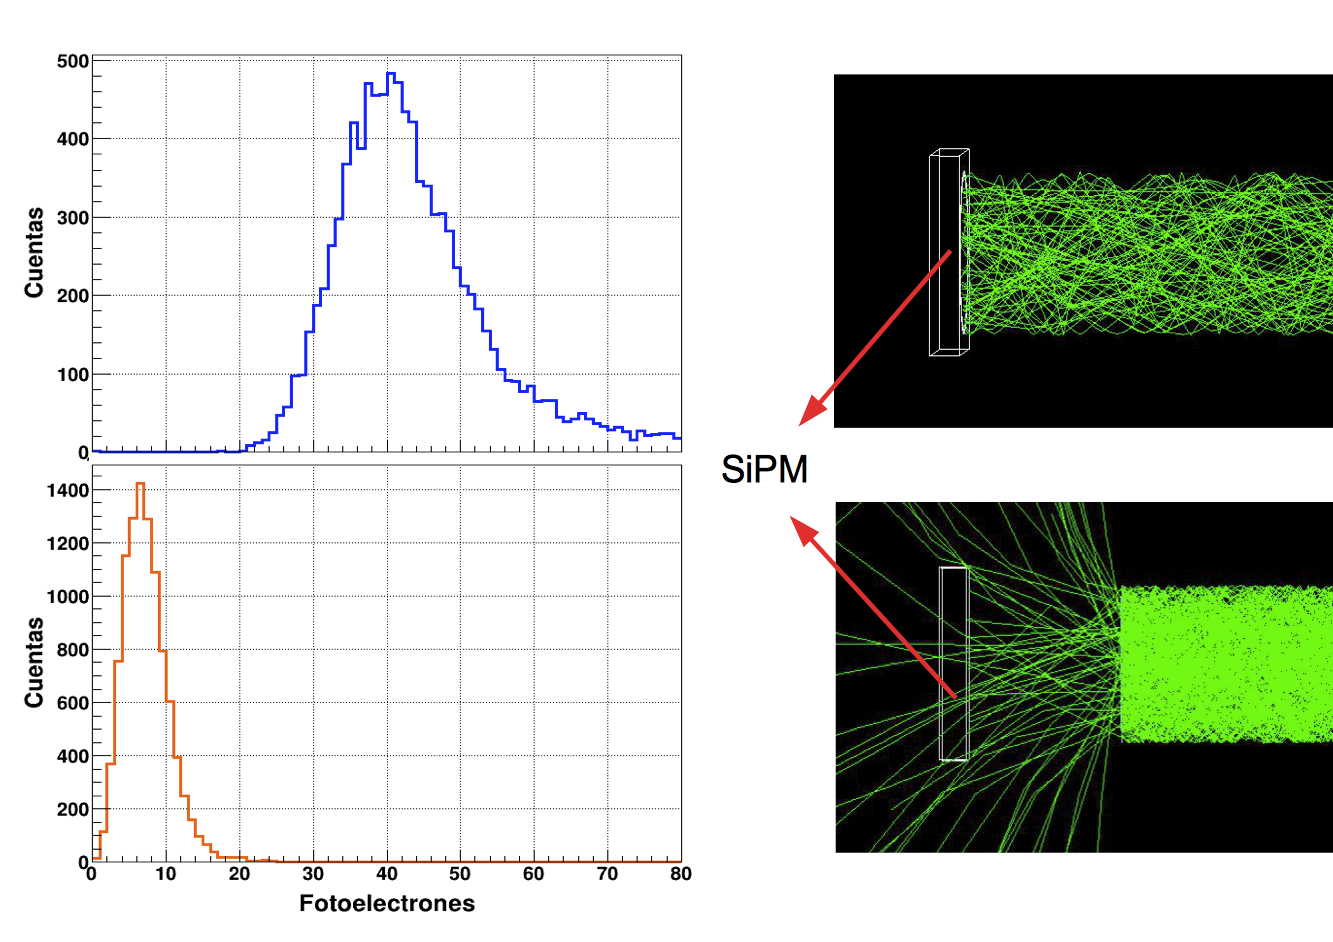
\includegraphics[scale=0.5]{perdida.png}
   \caption[Diferencia del número de fotoelectrones medidos con dos sistemas de acople entre el SiPM y la fibra]{Diferencia del número de fotoelectrones medidos con un sistema donde el SiPM está pegado a la fibra (caso 1, arriba) y con un SiPM separado a 1.15 mm de la fibra (caso 2, abajo). Se puede observar que en el segundo caso la señal obtenida es 80\% menor que en el caso ideal, por lo que es importante garantizar un acople \'optimo entre el SiPM y la fibra de cada detector de centelleo del MuTe.}\label{perdida}
\end{figure}

%%%%%%%%%%%%%%%%%%%%%%%%%%%%%%%
%%%%%%%%%   Section   %%%%%%%%%
%%%%%%%%%%%%%%%%%%%%%%%%%%%%%%%

\section{Respuesta del hodoscopio}\label{section_hodoscopio}
Determinar la respuesta de cada panel del hodoscopio consiste en contabilizar el número de fotoelectrones que se producen en una barra horizontal y una barra vertical. Por lo tanto, para el panel frontal del hodoscopio, se tiene que el n\'umero de fotoelectrones producidos en un pixel viene dado por 
\begin{equation}
\label{n_FE}
P^{F}_{i,j}=N^{F}_{i}+N^{F}_{j},
\end{equation}
donde $N^{F}_{i}$ y $N^{F}_j$ son el n\'umero de fotoelectrones producidos en la barra horizontal y en la barra vertical, respectivamente.
\begin{figure}[h!]
    \centering
        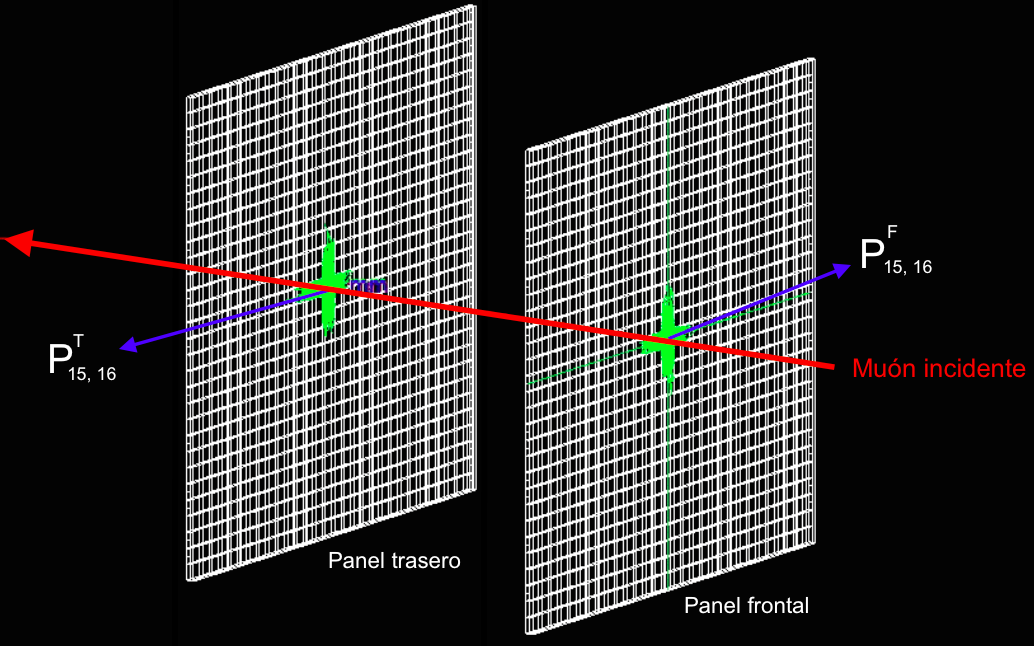
\includegraphics[scale=0.42]{panel_geant4.png}
   \caption[Respuesta del hodoscopio del MuTe simulado en Geant4]{Respuesta del hodoscopio del MuTe al paso de un muón de 3 GeV que ingresa de forma perpendicular a la superficie del panel frontal. En esta simulaci\'on se observa que para una dirección particular, los píxeles activados al paso de la partícula son $P^{F}_{15,16}$ y $P^{T}_{15,16}$ en el panel frontal y el panel trasero, respectivamente. Es decir, el mu'on entra perpendicularmente al panel.}\label{panel_geant4}
\end{figure}

A partir de los resultados obtenidos de la respuesta característica de una barra centelladora, se puede obtener la respuesta de un panel de detección a muones de 3 GeV. Por ejemplo, de la figura \ref{fotoelec_2cm} se tiene que $N^{F}_{i=1}=40$ y $N^{F}_{j=1}=40$, por lo que en el píxel $P^{F}_{1,1}$ se producen en promedio 80 fotoelectrones,
\begin{equation}
P^{F}_{1,1}=N^{F}_{i=1}+N^{F}_{j=1} = 40+40=80,
\end{equation}
al paso de un muón de 3 GeV, que incide en la dirección normal y en el punto medio del píxel. 

De la misma manera, se tiene que en el pixel $P^{F}_{30,30}$ se producen alrededor de 74 fotoelectrones:
\begin{equation}
P^{F}_{30,30}= N^{F}_{i=30}+N^{F}_{j=30}= 37+37 = 74.
\end{equation}
Siguiendo este procedimiento se obtiene el número promedio de fotoelectrones producidos por muones de 3 GeV, que han incidido en cada uno de los píxeles del panel, como se muestra en la figura \ref{atenuacion_panel_round}. 
\begin{figure}[h!]
    \centering
        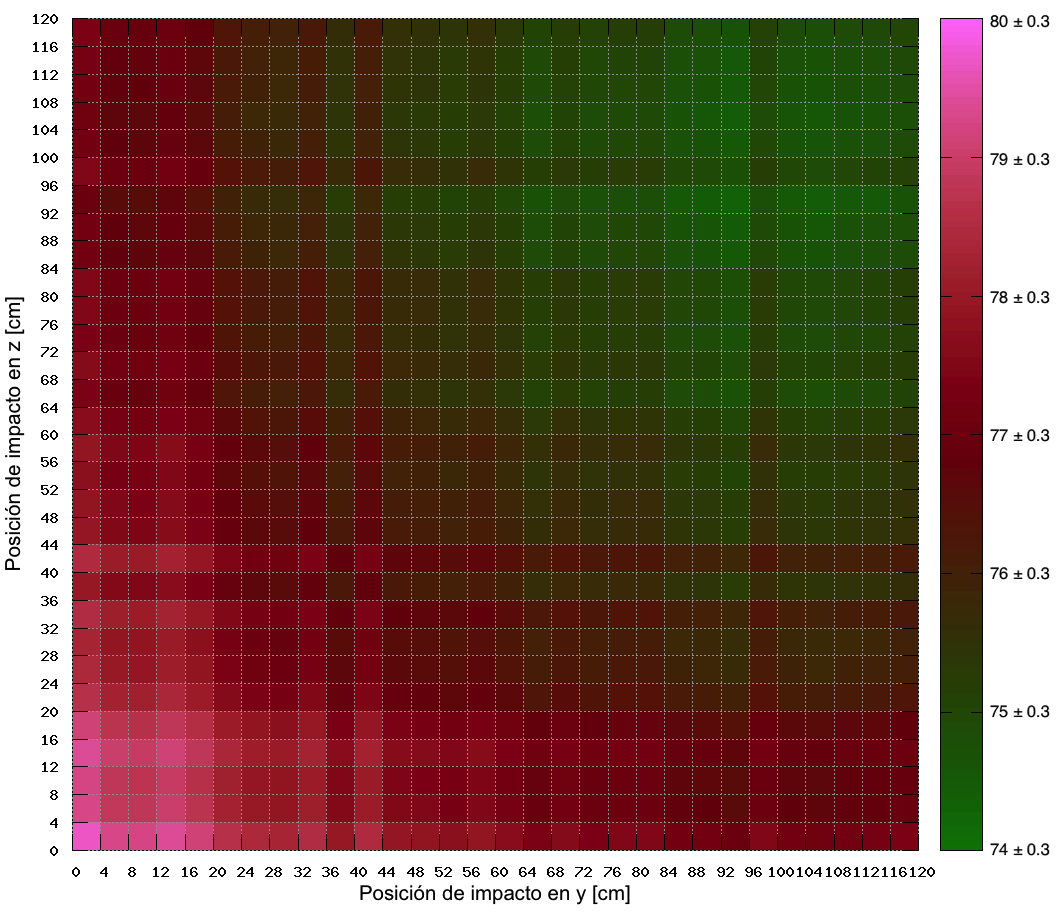
\includegraphics[scale=0.6]{atenuacion_panel_nuevo_2.png}
   \caption[Respuesta de los paneles del hodoscopio]{N\'umero promedio de fotoelectrones producidos en cada uno de los p\'ixeles de un panel del hodoscopio, por muones incidentes de 3 GeV de energ\'ia. Cada cuadro representa un pixel de detecci\'on y se puede observar que existe una diferencia entre las distintas zonas del panel. En el pixel $P_{11}$, donde el SiPM de la barra horizontal y de la barra vertical está a sólo 2 cm del punto de impacto del muón, se producen 80 fotoelectrones, mientras en que los pixeles correspondientes a la zona verde este n\'umero disminuye hasta 74. Este resultado es v\'alido tanto para el panel frontal como para el panel trasero.}\label{atenuacion_panel_round}
\end{figure}

Estos resultados son v\'alidos tanto para el panel frontal como para el panel trasero, y se observa que hay una diferencia de unos pocos fotoelectrones ($\approx 6$) entre las distintas zonas del gr\'afico \ref{atenuacion_panel_round}. Por ejemplo, en la zona verde definida por 44cm$\leq y \leq$120cm y 44cm$\leq z \leq$120cm, el n\'umero de fotoelectrones producidos est\'a alrededor de 75, mientras que en el resto del panel (zona rosa) se tienen alrededor de 79 fotoelectrones. Esta diferencia est\'a asociada a la atenuaci\'on de fotones en el detector de centelleo, es decir, los pixeles que est\'an m\'as cercanos al SiPM cuentan m\'as fotoelectrones. 

La inhomogeneidad en la respuesta de los paneles se debe a la geometría de los mismos. Es por esto que es necesario definir un umbral de detección de muones, es decir, se deben producir por encima de los 74 fotoelectrones en los pixeles de cada panel para registrar un evento.
%%%%%%%%%%%%%%%%%%%%%%
%%%%% CHAPTER 4  %%%%%
%%%%%%%%%%%%%%%%%%%%%%
\chapter{Detector MuTe: El detector Cherenkov de agua}\label{cap4}
Los detectores Cherenkov de agua se basan en la detección de la radiación Cherenkov producida cuando una partícula de alta energía atraviesa el agua, con una velocidad $v$ mayor a la velocidad de la luz $c$ en un medio con constante dieléctrica $\epsilon(\omega)$ \cite{Asorey-phd2012}, es decir, 
\begin{equation}
v > \frac{c}{\sqrt{\epsilon(\omega)}} \,\,\,\, \rightarrow \,\,\,\, \beta > \frac{1}{\sqrt{\epsilon(\omega)}}. 
\end{equation}
Las pérdidas de energía que sufre una partícula al atravesar una distancia $dl$ en el medio dispersor de densidad constante $\rho$, en el interior de un cilindro de radio $a$ cuyo eje coincide de la dirección de movimiento,
\begin{equation}
\frac{dE}{dl} = \rho \frac{dE}{dX},
\end{equation}
vienen dadas por
\begin{equation}
\label{Fermi}
\left ( \frac{dE}{dl} \right )_{b>a} = - ca \,\Re \left ( \int_{0}^{\infty} B_{3}^{*}(\omega) E_{1}(\omega)d\omega \right ),
\end{equation}
donde $E_1$ es la componente longitudinal del campo eléctrico, $B_3$ es la componente transversal del campo magnético, presentes en el medio, ambos funciones de la frecuencia $\omega$ y $b$ es el par\'ametro de impacto de la part\'icula medido sobre la l\'inea que da la direcci\'on del movimiento. Esta ecuación relaciona la pérdida diferencial de energía para regiones con $b>a$ luego de atravesar una cantidad de materia, $X$, en la dirección de movimiento \cite{Asorey-phd2012}.  

Si el medio es ligeramente absorbente la ecuación (\ref{Fermi}) se ve modificada y resulta la ecuación de Frank-Tamm (\ref{Frank-Tamm}), que muestra una fuerte dependencia en la frecuencia para la emisión de fotones Cherenkov,
\begin{equation}
\label{Frank-Tamm}
\left ( \frac{dE}{dl} \right )_{Cherenkov} = \left(\frac{Z e}{c} \right)^2  \int_{\beta^2\epsilon(\omega)>1}  \omega \left (1- \frac{1}{\beta^2\epsilon(\omega)}\right ) d\omega,
\end{equation}
donde $Z$ es el n\'umero at\'omico. Para el agua y en el rango del espectro visible, esta radiación se produce en longitudes de onda cortas, donde el índice de refracción $n= \sqrt{\epsilon(\omega) \mu(\omega)} \approx \sqrt{\epsilon(\omega)}$ aumenta levemente con la frecuencia. Esto se puede observar en la figura (\ref{asorey1}).
\begin{figure}
    \centering
    \begin{subfigure}{0.45\textwidth}
        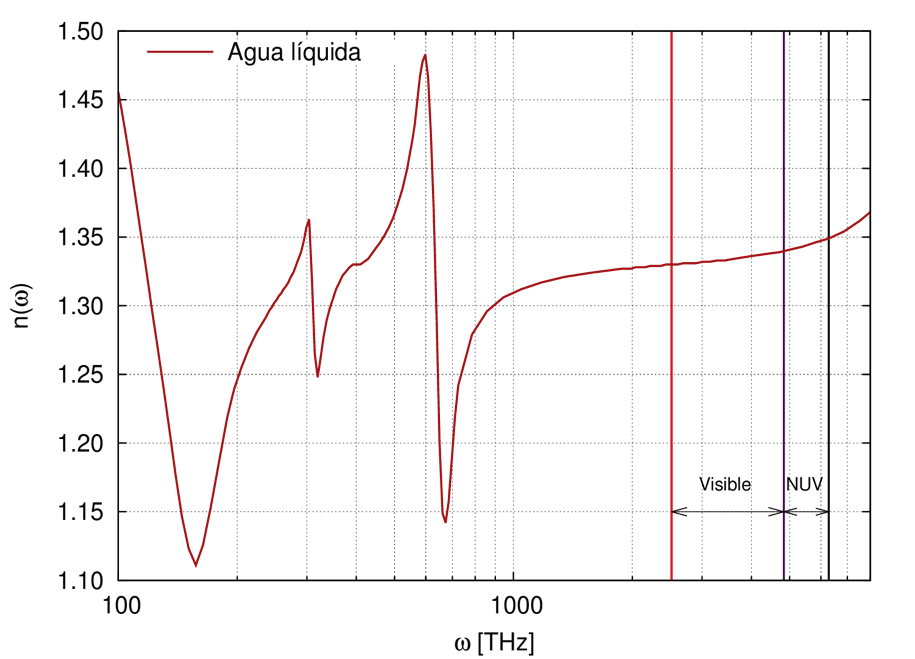
\includegraphics[width=\textwidth]{asorey1.png}
        \caption{}
        \label{asorey1}
    \end{subfigure}
        \begin{subfigure}{0.45\textwidth}
        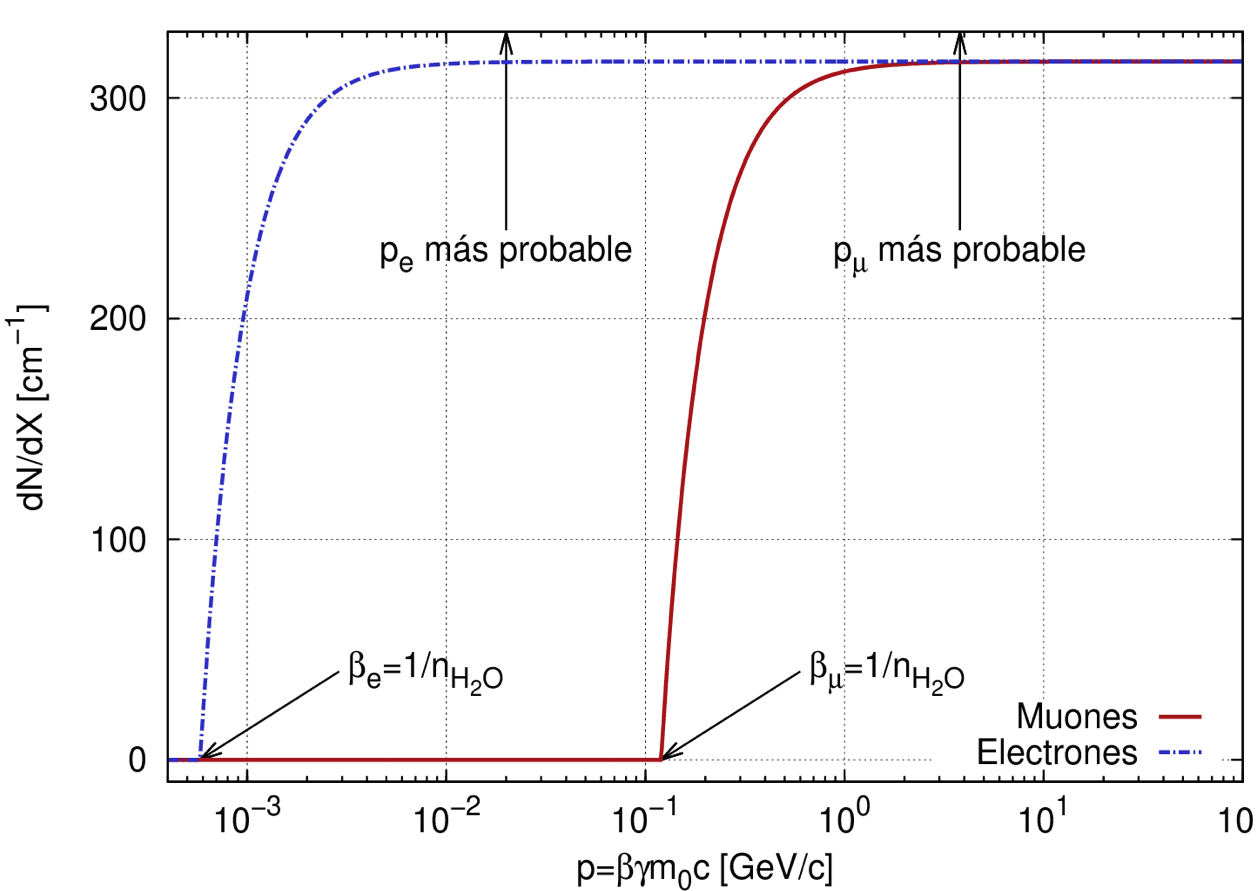
\includegraphics[width=\textwidth]{asorey2.png}
        \caption{}
        \label{asorey2}
    \end{subfigure}
   \caption[Índice de refracción del agua líquida como función de la
frecuencia angular y producción de fotones Cherenkov en la banda visible y NUV]{(a) Índice de refracción del agua líquida ($n(\omega)\approx \sqrt{\epsilon(\omega)}$) como función de la
frecuencia angular $\omega$. La banda visible se tiene entre 400 y 790 THz. (b) Producción de fotones Cherenkov en la banda 300nm $< \lambda < 570$nm (visible
y NUV) como función del impulso de un electrón (puntos y rayas) y de un
muón (línea sólida), al recorrer 1 cm en agua líquida. En este caso la cantidad de fotones tiende a un valor constante de 315 fotones por centímetro (figura tomada de \cite{Asorey-phd2012}).}\label{asorey}
\end{figure}
El rango de frecuencias de interés para el WCD del MuTe está entre el visible y el cercano ultravioleta, donde $n(\omega)$ se puede considerar constante y el número de fotones $N$ producidos en un intervalo de longitudes de onda $\lambda_1$ y $\lambda_2$ es
\begin{equation}
N = 2\pi \alpha_{EM} l \left( 1 - \frac{1}{\beta^2 n^2}\right)  \left(\frac{1}{\lambda_2} - \frac{1}{\lambda_1}\right),
\end{equation}
donde $\alpha_{EM}=(e^2/\hbar c)$ es la constante de estructura fina.

El número de fotones Cherenkov producidos por una partícula con impulso, $p$, al recorrer una longitud, $l$, en un medio con índice de refracción, $n$, se puede determinar a partir de 
\begin{equation}
\beta(p)= \left[1 + \left(\frac{m_0 c}{p}\right)^2 \right]^{-1/2}
\end{equation}
siempre que $\beta > 1/n$. Los fotones emitidos por unidad de longitud tienden rápidamente a un valor constante, que sólo depende del rango de longitudes de onda considerado, del índice de refracción del medio y de la distancia recorrida (ver figura \ref{asorey2}). 

La radiación Cherenkov se propaga en la dirección dada por el vector de Poynting, donde el ángulo de emisión $\theta_c$ viene dado por  
\begin{equation}
\label{angulo}
\cos \theta_c = \frac{1}{\beta \sqrt[]{\epsilon(\omega)}}.
\end{equation}

En general, la respuesta de un WCD al flujo de part\'iculas secundarias, est\'a dominada por las componentes electromagnética y muónica del flujo \cite{Asorey-phd2012}. A continuaci\'on se muestra la respuesta del WCD del MuTe ante muones y electrones monoenergéticos, que ingresan verticalmente al detector. Para esto se ha desarrollado un código en Geant4 que permite estimar el número de fotones Cherenkov producidos por la partícula incidente, la fracción de estos fotones que logran tocar la superficie externa del fotoc\'atodo del PMT y la cantidad de fotoelectrones que se producen por efecto fotoeléctrico. Además, se puede estimar el pulso promedio y la distancia recorrida en el agua por la partícula al producir esta señal.

%%%%%%%%%%%%%%%%%%%%%%%%%%%%%%%
%%%%%%%%%   Section   %%%%%%%%%
%%%%%%%%%%%%%%%%%%%%%%%%%%%%%%%

\section{Descripción}
El WCD del MuTe está compuesto por un contenedor metálico de agua, un material reflector y dispersivo de luz (Tyvek) y un fotomultiplicador con cierta eficiencia cuántica para detectar fotones.

\subsection{El contenedor, el Tyvek y el agua}
El contenedor del agua simulado es un cubo de longitud $l_c=$1.21 m, de acero inoxidable. El agua ocupa un cubo de $l=$1.20 m de lado con índice de refracción $n$, que var\'ia entre 1.3435 y 1.3608, y una longitud de absorción de fotones que va desde los 0.69 m a los 2.90 m según su energía. En las paredes del cubo de agua se define el Tyvek como una superficie óptica con índice de reflexión $n_{Tyvek}=1$, que difunde los fotones Cherenkov.

\begin{figure}[h!]
    \centering    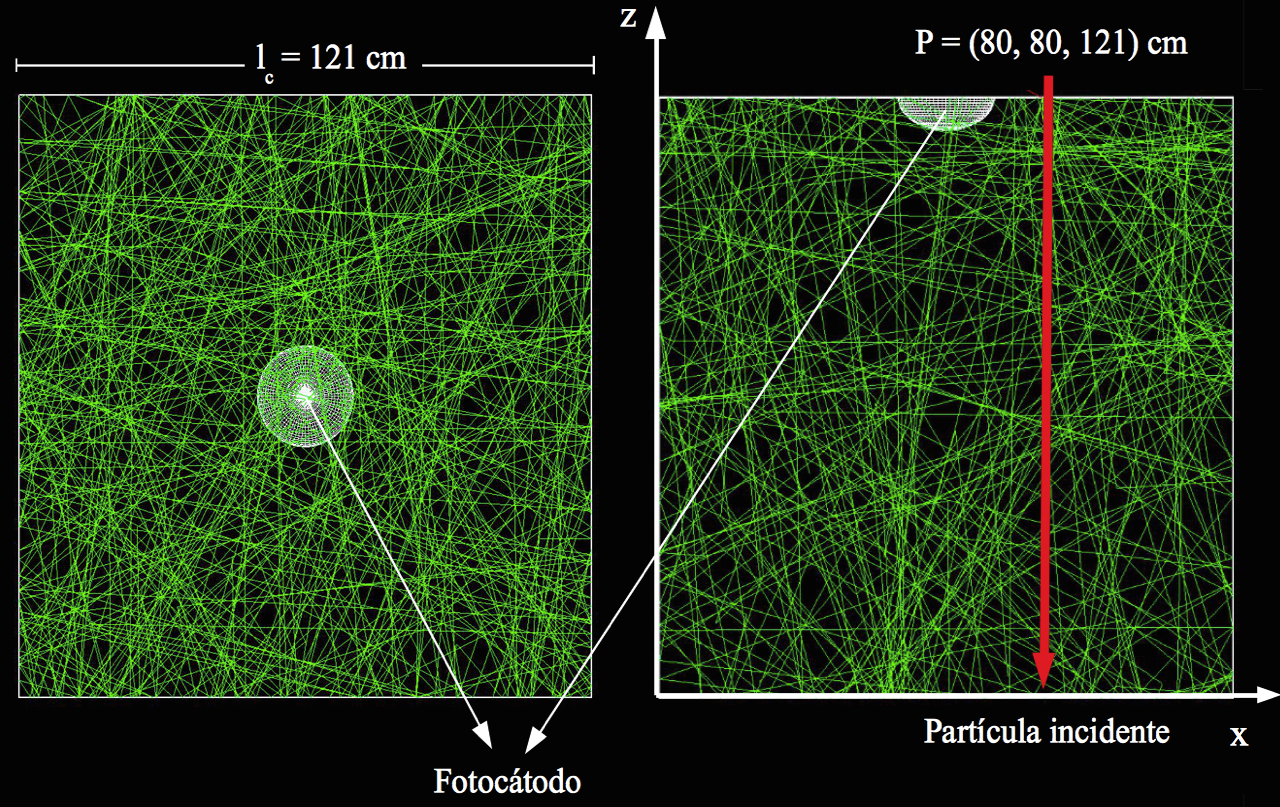
\includegraphics[width=\textwidth]{wcd_punto.png}
   \caption[Geometría del WCD del MuTe simulado en Geant4]{Geometría del WCD del MuTe simulado en Geant4, vista longitudinalmente (derecha) y transversalmente (izquierda). El cubo exterior de 121 cm de lado es de acero inoxidable y contiene el agua. Entre estos dos volúmenes se encuentra el Tyvek, que difunde los fotones Cherenkov (líneas verdes) hacia dentro del detector. La semielipse blanca representa el fotocátodo del PMT, donde se ha definido la eficiencia cu\'antica del mismo para detectar fotones seg\'un su energ\'ia. A la derecha se observa el sistema de coordenadas utilizado y el punto $P$ desde donde se lanzan las partículas.}\label{wcd}
\end{figure}
\begin{comment}
\begin{figure}[h!]
    \centering    \includegraphics[width=\textwidth]{wcd.png}
   \caption[Geometría del WCD simulado en Geant4]{Geometría del WCD simulado en Geant4. La semielipse amarilla representa el fotocátodo del PMT, donde se ha definido la eficiencia cu\'antica del mismo para detectar fotones seg\'un su energ\'ia.}\label{wcd}
\end{figure}
\end{comment}
\subsection{El Fotomultiplicador}
Para el tubo fotomultiplicador (de referencia R5912 de Hammamatsu), se simuló el fotocátodo como un semielipsoide de aire con semiejes $s_x=$10.1 cm, $s_y=$10.1 cm y $s_z=$6.5 cm, ubicado en la parte superior del cubo de agua (ver figura \ref{wcd}). La eficiencia cuántica de este dispositivo se introdujo en el código, de modo que los fotones que alcancen tocar la superficie externa del fotocátodo sean absorbidos o detectados según la probabilidad de detección. \'Esta depende de la longitud de onda $\lambda$, como se muestra en la figura (\ref{QEPMT}) y se tiene que el valor máximo de probabilidad de detección es del 25\% para fotones con $\lambda =$ 400 nm\footnote{\url{http://pdf.datasheetcatalog.com/datasheet/hamamatsu/R5912.pdf}}. A los fotones detectados, es decir, aquellos fotones que tengan la energía suficiente para liberar un electrón de la superficie del fotoc\'atodo por efecto fotoeléctrico, se les denomina fotoelectrones.
\begin{figure}[h!]
    \centering
        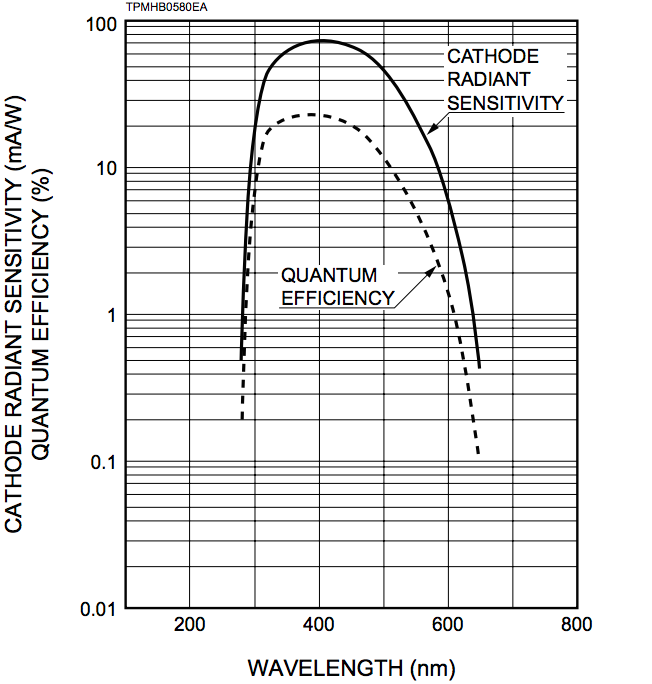
\includegraphics[scale=0.35]{QEPMT.png}
   \caption[Eficiencia cuántica del PMT R5912 de Hamamatsu]{Eficiencia cuántica del PMT R5912 de Hamamatsu, tomada de \url{http://pdf.datasheetcatalog.com/datasheet/hamamatsu/R5912.pdf}.}\label{QEPMT}
\end{figure}

Cabe destacar que la inclusi\'on de la eficiencia del PMT en el c\'odigo, como una funci\'on dependiente de $\lambda$, representa una mejora respecto a las simulaciones de WCDs realizadas anteriormente dentro del grupo de investigaci\'on. En el trabajo de \cite{Calderon-Ardila2015}, se toma una eficiencia única del 25\%, para el rango de longitudes de onda entre 330 nm y 570 nm \cite{calderon2015geant4}. Por lo tanto, el nuevo c\'odigo ofrece resultados m\'as precisos de los pulsos producidos al paso de part\'iculas en el agua. Además, \'este permite estimar la respuesta de los WCDs ante todo el flujo de partículas secundarias de un sitio particular, mientras que en \cite{calderon2015geant4} se seleccionan ciertas partículas para ser inyectadas una a una en el detector. Los detalles sobre esta metodología se muestran en la secci\'on \ref{WCDFLUJOR} y, el c\'odigo en el apéndice \ref{apendice}. 

%%%%%%%%%%%%%%%%%%%%%%%%%%%%%%%
%%%%%%%%%   Section   %%%%%%%%%
%%%%%%%%%%%%%%%%%%%%%%%%%%%%%%%

\section{Respuesta del WCD ante muones y electrones}
\begin{figure}[h!]
    \centering
        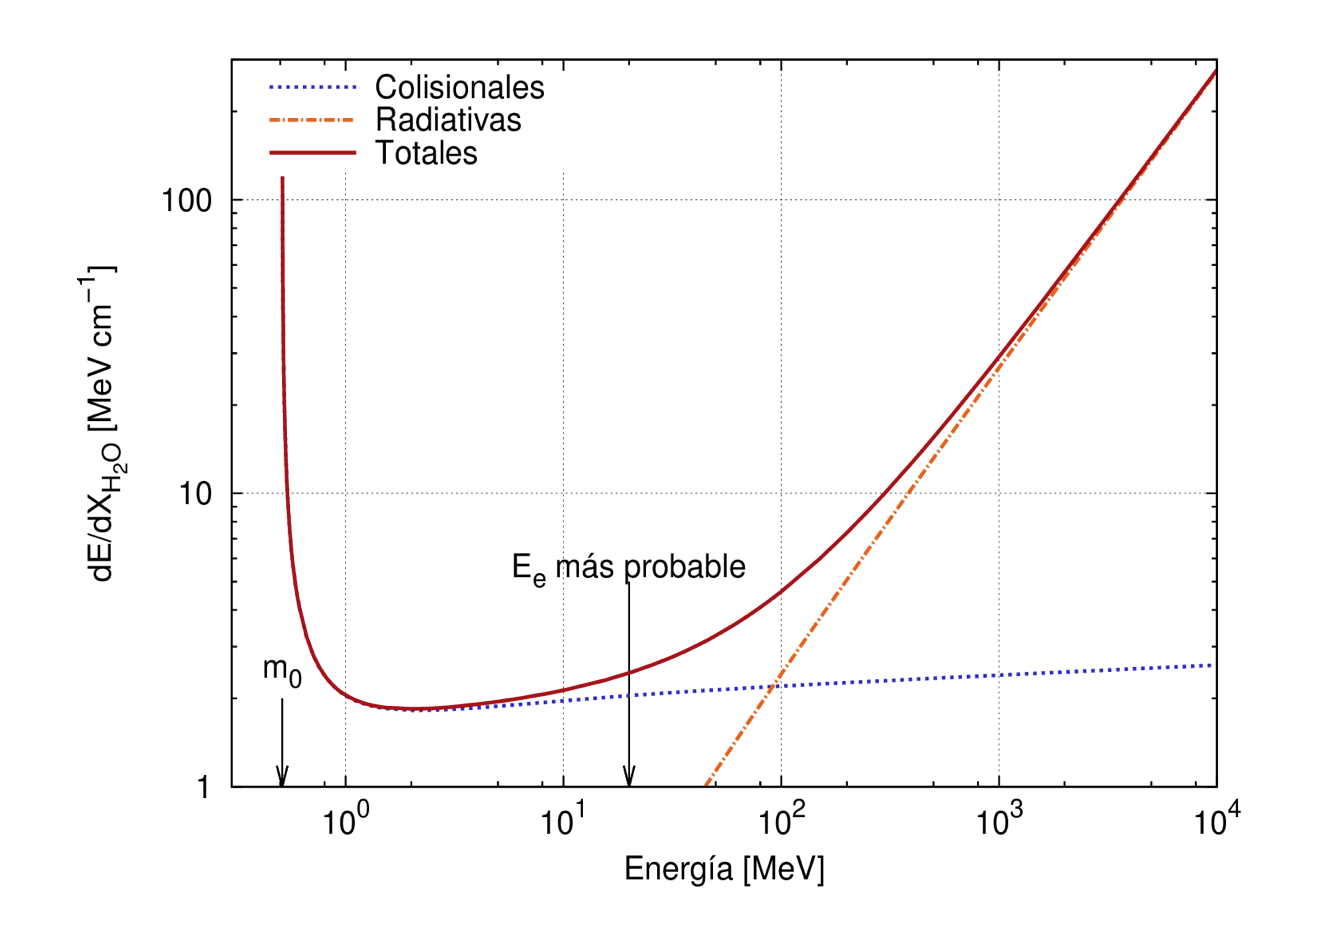
\includegraphics[scale=0.4]{stopping_e.png}
   \caption[Poder de frenado del electrón en agua líquida]{Poder de frenado $dE/dX$ para electrones moviéndose a través de agua líquida como función de la energía del electrón en el rango 103 $<$ E/MeV $<$ 104. Se muestran las contribuciones radiativas (puntos y rayas), las pérdidas debidas a colisiones (punteado) y la suma de ambos términos (línea sólida), figura tomada de \cite{Asorey-phd2012}.}\label{stopping_e}
\end{figure}
%Toda partícula cargada de masa en reposo $m_0$ producirá una señal Cherenkov en el agua si su impulso $p$ cumple lo siguiente \cite{Asorey-phd2012}
%\begin{equation}
%p_{Ch} \geq 1.1339cm_0.
%\end{equation} 
El umbral de energ\'ia para la emisión fotones Cherenkov por parte de los electrones es $E^e_{Ch}=0.773$ MeV \cite{Asorey-phd2012}. La energía típica de los electrones atmosféricos es del orden de los MeV, como se observa en la figura (\ref{flujo}) a nivel del Volc\'an Cerro Mach\'in. Con un poder de frenado en el agua dado por la figura (\ref{stopping_e}), un electrón de 20 MeV recorre alrededor de 10 cm antes de ser absorbido en el agua.

Por otra parte, la energía depositada por los muones atmosféricos que penetran el detector permanece constante, y se aproxima al valor 
\begin{equation}
\frac{dE}{dx}_{H_2O} \simeq 2 \text{MeV/cm}.
\end{equation}
A partir de lo anterior, se puede afirmar que un muón atmosférico con energía típica de 3 GeV es capaz de recorrer varios metros en agua o en roca \cite{Asorey-phd2012}. La respuesta del WCD ante estas partículas depende de la deposición de energía, la producción de fotones Cherenkov y la geometría del detector. 

\subsection{Detección de muones verticales}
Para medir la energía depositada por las partículas incidentes se necesita una calibración absoluta del detector, por lo que generalmente se adopta la unidad de medida del Muón Vertical Equivalente (VEM) \cite{AEtchegoyen-etal2005}. \'Esta se define como la carga promedio colectada en el PMT cuando un muón de alta energía atraviesa todo el detector de manera vertical. En la calibración de los WCD estos muones se pueden identificar fácilmente instalando centelladores plásticos encima y debajo del detector, centrados en su eje \cite{AEtchegoyen-etal2005}, de modo que el muón puede ser detectado antes y después de salir del WCD.

En la simulación del detector no es necesario implementar este método, pues el código de Geant4 permite inyectar muones con una energía y dirección inicial escogida. En este caso se inyectaron 100000 muones con 3 GeV de energía inicial, en dirección $-\hat{z}$ hacia el agua y la posición inicial dada por el punto $P = (80, 80, 121)$ cm, justo sobre el WCD como se muestra en la figura \ref{wcd}. A partir de esto se obtiene el número promedio de fotones Cherenkov, $N$, que se producen en el agua al paso de estas partículas (figura \ref{cherenkov_total_mu}). Una porción de $N$ logra alcanzar la superficie externa del fotoc\'atodo, denominados como $N_{\mathrm{PMT}}$ (figura \ref{al_pmt_mu}). Finalmente, los $N_{\mathrm{PMT}}$, producen un n\'umero de fotoelectrones, $N_{\mathrm{FE}}$, dependiendo de su longitud de onda. Los $N_{\mathrm{FE}}$ son contabilizados para obtener la carga depositada por un VEM, como se muestra en la figura (\ref{fotoelectrones_vem}). Con el ajuste gaussiano se obtiene el pico de este \'ultimo histograma, que está centrado alrededor de los 203 fotoelectrones.

\begin{figure}
    \centering
    \begin{subfigure}{0.45\textwidth}
        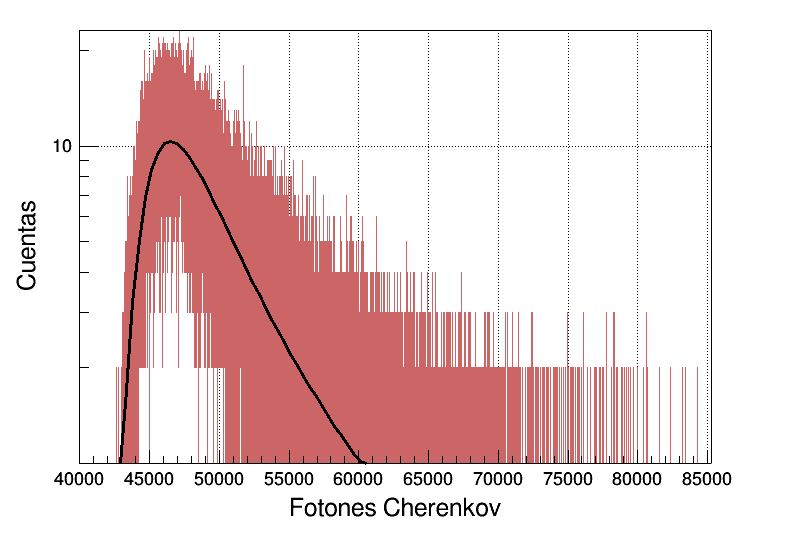
\includegraphics[width=\textwidth]{cherenkov_total_mu.png}
        \caption{}
        \label{cherenkov_total_mu}
    \end{subfigure}
    \begin{subfigure}{0.45\textwidth}
        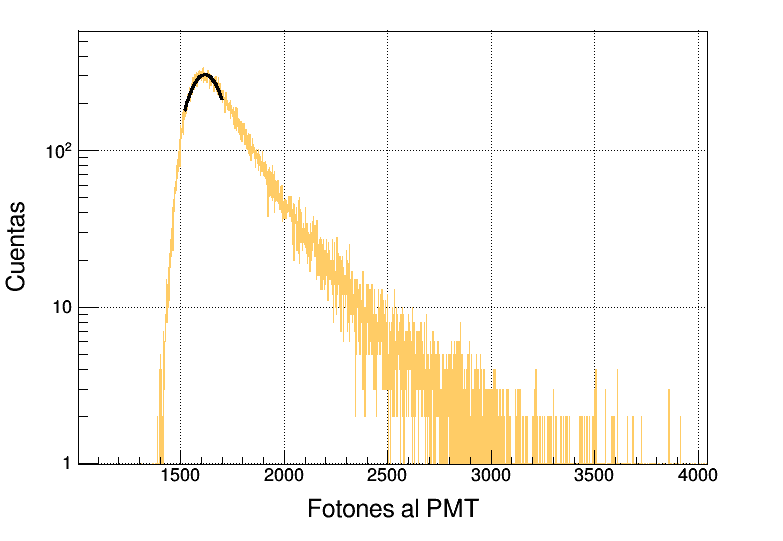
\includegraphics[width=\textwidth]{al_pmt_mu.png}
        \caption{}
        \label{al_pmt_mu}
    \end{subfigure}
    \begin{subfigure}{0.45\textwidth}
        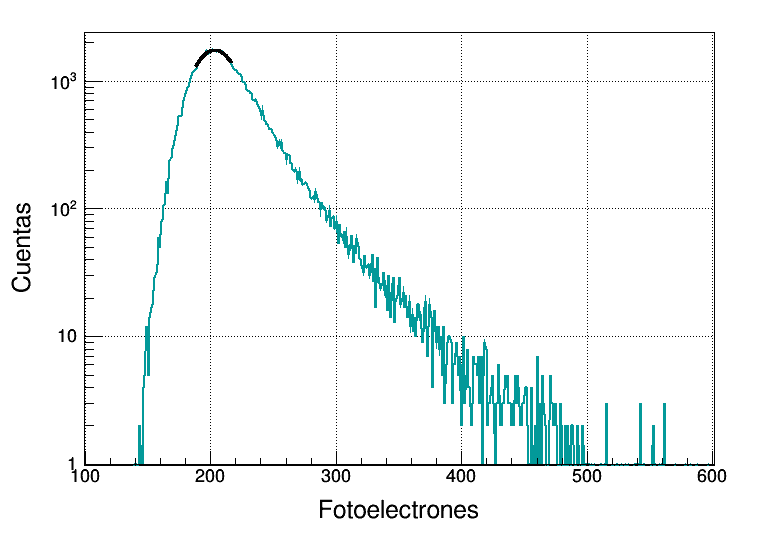
\includegraphics[width=\textwidth]{fotoelectrones_vem.png}
        \caption{}
        \label{fotoelectrones_vem}
    \end{subfigure}
    \begin{subfigure}{0.45\textwidth}
        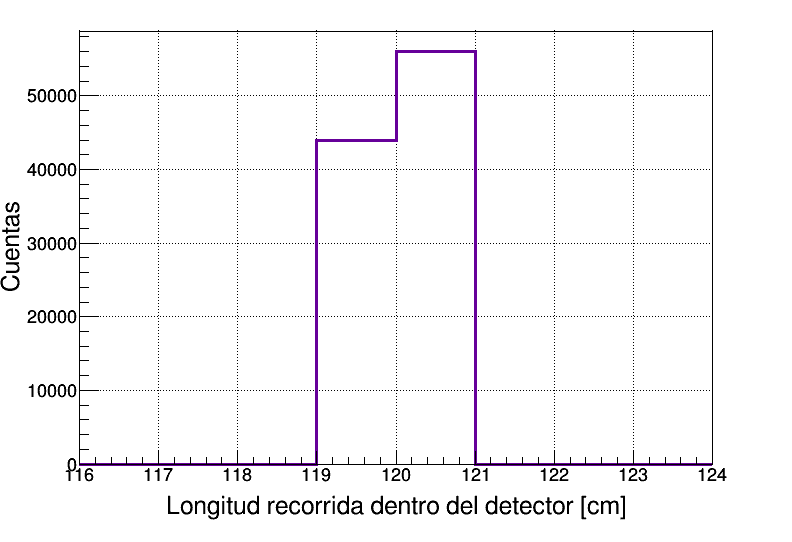
\includegraphics[width=\textwidth]{distancia_vem.png}
        \caption{}
        \label{distancia_vem}
    \end{subfigure}
    \caption[Número de fotones Cherenkov producidos en el WCD, fotones que alcanzan la superficie del fotoc\'atodo del PMT y fotoelectrones generados por muones verticales de 3 GeV]{Número de (a) fotones Cherenkov producidos producidos en el WCD, (b) fotones que alcanzan la superficie externa del fotoc\'atodo del PMT y (c) fotoelectrones generados por 100000 muones de 3 GeV que ingresan de forma vertical y recorren una distancia (d). Se observa que el pico de (a) está centrado en 46857 fotones, el de (b) está en 1617 y el de (c) en 203 fotoelectrones, siendo esta \'ultima la unidad de medida VEM para el WCD del MuTe. Además se tiene que alrededor de 60000 muones atraviesan por completo el WCD, es decir, recorren 120 cm en el agua.}\label{VEM_plots}
\end{figure}

Además, la simulación permite evaluar la eficiencia del WCD ante muones, es decir, en promedio se tiene que un VEM de 3 GeV genera alrededor de 46857 fotones Cherenkov en el agua, sólo 1617 de estos fotones alcanzan la superficie externa del fotoc\'atodo y a partir de su eficiencia cuántica se generan alrededor de 203 fotoelectrones en total. Así el sistema tiene una eficiencia de detección de muones del 0.4\%, es decir, 
\begin{equation}
\eta_{\mathrm{WCD}}=\frac{N_{\mathrm{FE}}}{N} 100\%=\frac{203}{46857}100\%=0\textnormal{.}4\%
\end{equation}

La simulación también arroja la distancia $l$ recorrida por las partículas en el agua, como se muestra en la figura (\ref{distancia_vem}), que está linealmente relacionada con el número de fotones Cherenkov, $N$, que se producen. 


\subsection{Detección de electrones verticales}
Para analizar la respuesta de WCD ante electrones de energía típica (20 MeV) se inyectaron 100000 electrones de manera vertical hacia el detector desde una posición fija, dada por el punto $P=(80, 80, 121)$ cm de la figura \ref{wcd}, obteniendo los resultados que se muestran en la figura \ref{VE_plots}. De aquí se tiene que el número de fotones Cherenkov producidos en promedio es de 3538 (figura \ref{cherenkov_total_e}), mientras que los que llegan al PMT son alrededor de 132 fotones (figura \ref{al_pmt_e}), generando 17 fotoelectrones (figura \ref{fotoelectrones_vee}).

La distancia recorrida en el agua por estos electrones varía desde los 2 cm hasta los 12 cm, lo que explica el bajo número de fotones Cherenkov producidos en este caso respecto al VEM, ver figura (\ref{distancia_vee}).

\begin{figure}[h!]
    \centering
    \begin{subfigure}{0.45\textwidth}
        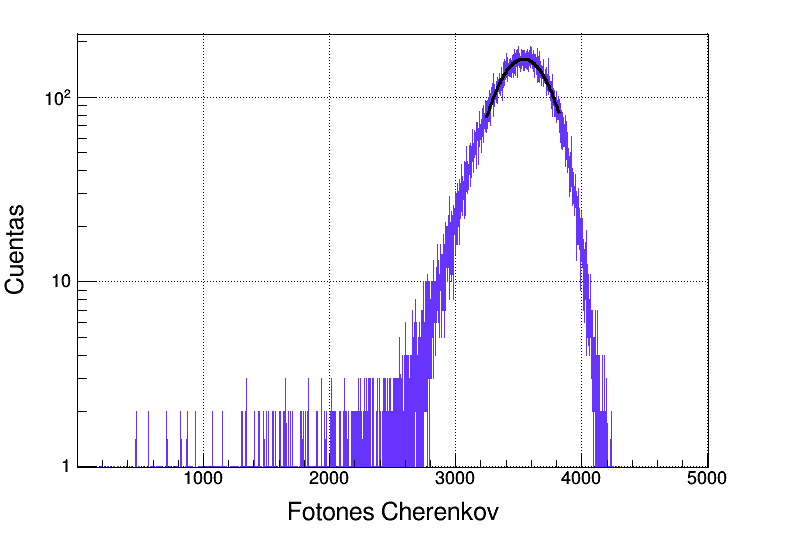
\includegraphics[width=\textwidth]{cherenkov_total_e.png}
        \caption{}
        \label{cherenkov_total_e}
    \end{subfigure}
    \begin{subfigure}{0.45\textwidth}
        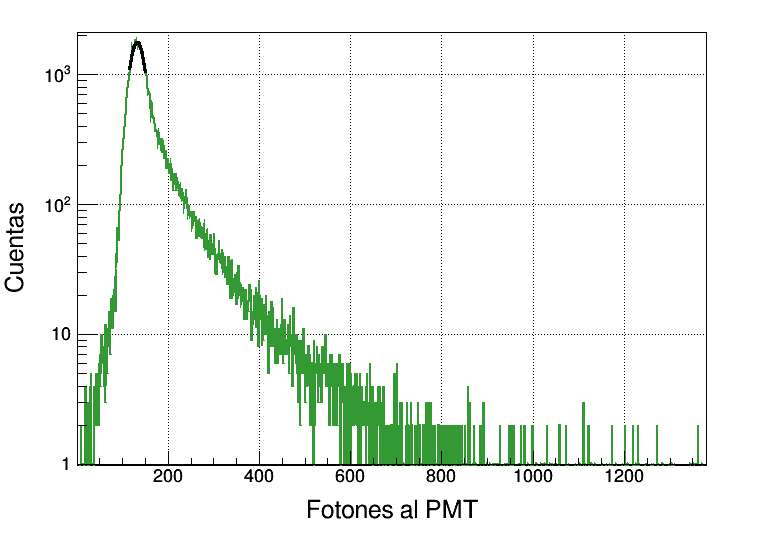
\includegraphics[width=\textwidth]{al_pmt_e.png}
        \caption{}
        \label{al_pmt_e}
    \end{subfigure}
    \begin{subfigure}{0.45\textwidth}
        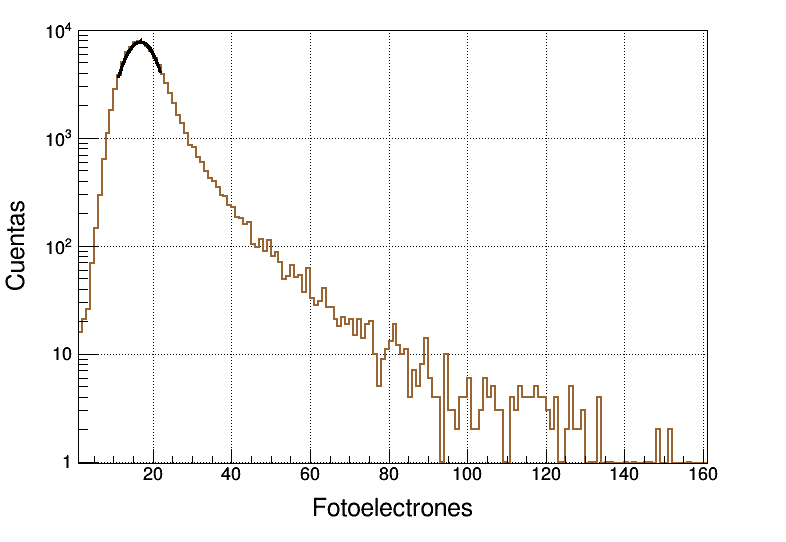
\includegraphics[width=\textwidth]{fotoelectrones_vee.png}
        \caption{}
        \label{fotoelectrones_vee}
    \end{subfigure}
    \begin{subfigure}{0.45\textwidth}
        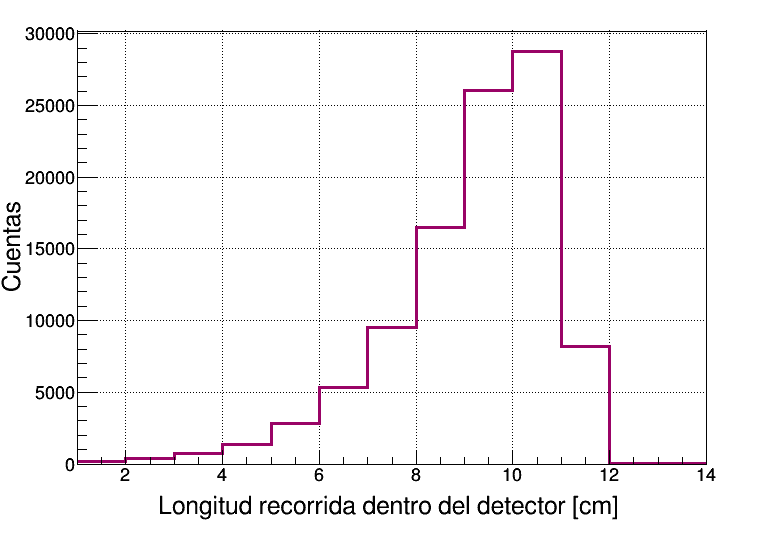
\includegraphics[width=\textwidth]{distancia_vee.png}
        \caption{}
        \label{distancia_vee}
    \end{subfigure}
    \caption[Número de fotones Cherenkov producidos en el WCD, fotones que alcanzan la superficie externa del fotoc\'atodo del PMT y fotoelectrones generados por electrones verticales de 20 MeV]{Número de (a) fotones Cherenkov producidos, (b) fotones que alcanzan la superficie externa del fotoc\'atodo y (c) fotoelectrones producidos por 100000 electrones de 20 MeV que ingresan al WCD de forma vertical y recorren una distancia (d) en el agua. Se tiene que el pico de (a) está centrado en 3538 fotones, el de (b) está en 132 y el de (c) en 17 fotoelectrones. En este caso los electrones alcanzan a recorrer un máximo de 11 cm en el agua que representa un 9.2\% de la longitud total vertical del WCD. El pico de (d) está alrededor de 10 cm.}\label{VE_plots}
\end{figure}


\subsection{Señal producida por muones y electrones verticales} 
Comparando los resultados obtenidos para muones y electrones verticales, y tomando el VEM como unidad de calibración, se tiene que el número promedio de fotoelectrones producidos por un electrón vertical (VE), representa sólo el 8\% de la señal depositada por el VEM (ver figura \ref{vem_vee}). También se observa que los electrones alcanzan a recorrer apenas 10 cm en el agua (figura \ref{distancia_vee}), debido a su poder de frenado (figura \ref{stopping_e}), produciendo un 7.5\% del número de fotones Cherenkov que generan los muones verticales (figura \ref{cherenkov_total_e}). Por lo tanto se puede decir que la señal depositada por un electrón de energía típica es mucho menor que la de un muón de energía típica, en el sitio de observación. Esto permite al detector MuTe diferenciar los muones de los electrones, como se puede comparar en el cuadro 4.1.

La señal en un detector real viene dada por un pulso característico, que en este caso se ha definido como el número de fotoelectrones registrados en un tiempo $t$. Los histogramas obtenidos para muones y electrones se han construido de forma tal, que se pueda obtener el número de fotoelectrones en ventanas temporales de 25 ns, ya que la electr\'onica de adquisici\'on del WCD opera con esta ventana de tiempo. En la figura \ref{Pulsos_mu_e} se puede observar que el pulso generado por un muón vertical de 3 GeV tiene una amplitud máxima de 88 fotoelectrones en los primeros 25 ns, mientras que el electrón deposita alrededor de 11 fotoelectrones en la misma ventana temporal. Ambos pulsos tienen aproximadamente la misma duración temporal pero uno se atenúa más rápidamente que el otro.

El tiempo de atenuación $\tau$ del pulso se obtiene a partir del ajuste exponencial dado por la función
\begin{equation}
y = A e^{-b\, t },
\end{equation}
donde 
\begin{equation}
\tau = \frac{1}{b}.
\end{equation}
Para el pulso promedio del muón se tiene que $b_{\mu^-}=0$.023740 ns$^{-1}$, de modo que el tiempo de atenuación es $\tau_{\mu^-}=42$.12 ns mientras que para el pulso del electrón de 20 MeV se tiene $b_{e^-}=0$.03053 ns$^{-1}$, dando un tiempo de atenuación $\tau_{e^-}=32$.75 ns, es decir, la señal del electrón decae más rápido que la señal producida por el muón (alrededor de 9.37 ns antes), como se muestra en la figura \ref{Pulsos_mu_e}, donde las curvas negras representan el ajuste exponencial de cada pulso.

Por otra parte la longitud de atenuación $l_a$ representa la distancia recorrida por los fotones Cherenkov antes de ser absorbidos en el agua o en el Tyvek, y viene dada por
\begin{equation}
l_a = \frac{\tau c}{n},
\end{equation}
donde $\tau$ es el tiempo de atenuación, $c$ la velocidad de la luz en el vacío y $n$ el índice de refracción del agua. Tomando $n=1$.34 se tiene la longitud de atenuación media, $l^{e^-}_a =$ 7.332 m y $l^{\mu^-}_a =$9.430 m, para electrones y muones, respectivamente.

\begin{figure}[h]
    \centering
        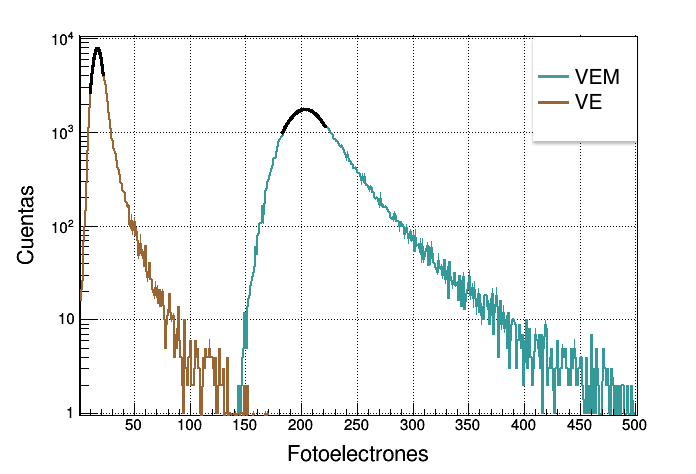
\includegraphics[scale=0.45]{vem_vee.png}
   \caption[Número de fotoelectrones producidos por la incidencia vertical de muones de 3 GeV (VEM) y electrones de 20 MeV (VE) sobre el WCD]{Número de fotoelectrones producidos por la incidencia vertical de muones de 3 GeV (VEM) y electrones de 20 MeV (VE) sobre el WCD. El número medio de fotoelectrones del VE es aproximadamente 17 (con $\sigma$ = 4.5) y representa un 8\% del número medio de fotoelectrones del VEM, aproximadamente 203 con   $\sigma$ = 20.}\label{vem_vee}
\end{figure}
\begin{figure}[h!]
    \centering
    \begin{subfigure}{0.45\textwidth}
        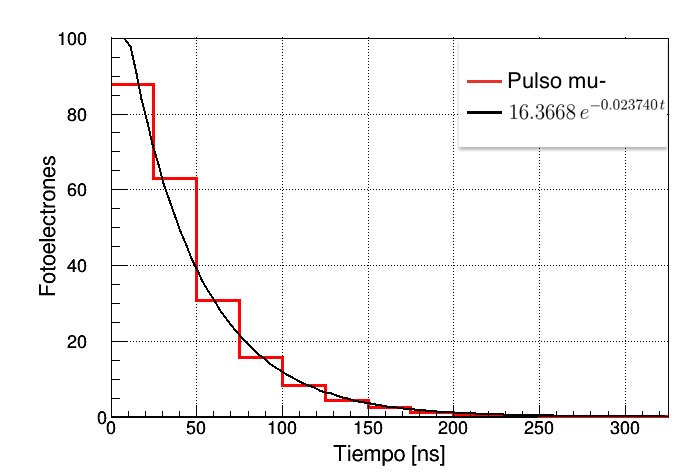
\includegraphics[width=\textwidth]{vem_tiempo.png}
        \caption{}
        \label{vem_tiempo}
    \end{subfigure}
     \begin{subfigure}{0.4\textwidth}
        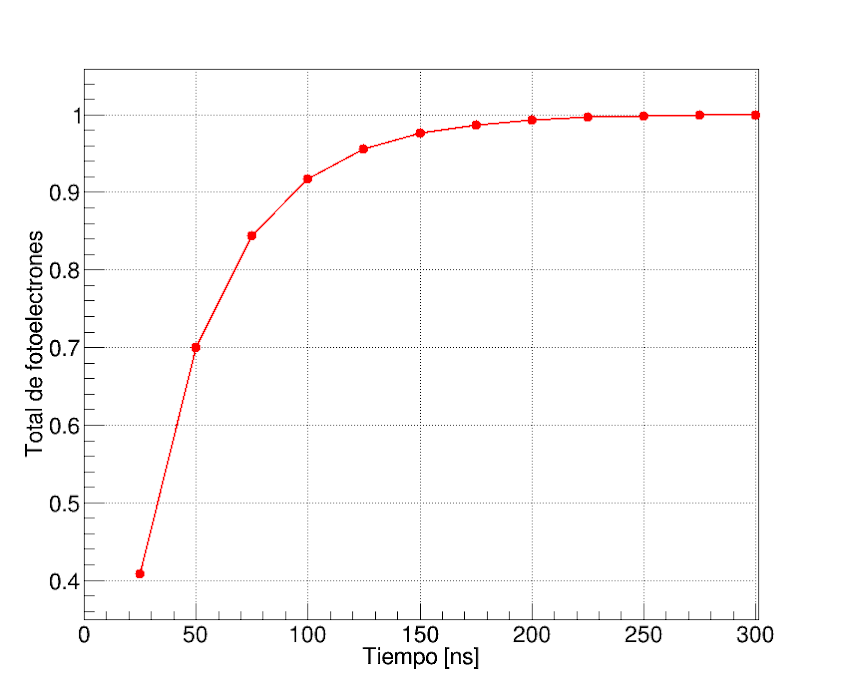
\includegraphics[width=\textwidth]{VEMcum.png}
        \caption{}
        \label{VEMcum}
    \end{subfigure}
    \begin{subfigure}{0.45\textwidth}
        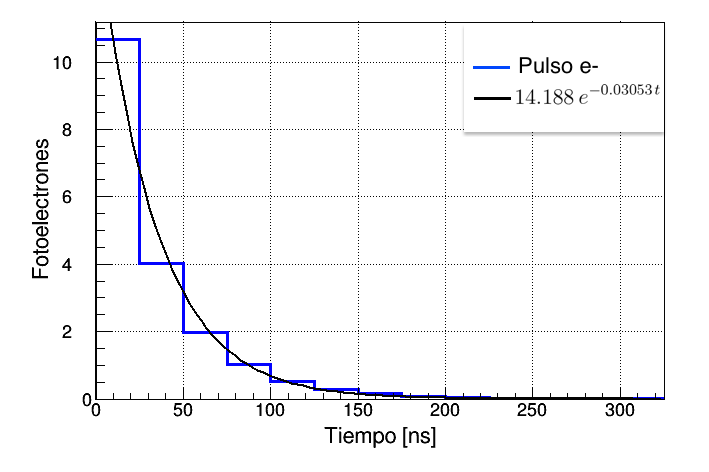
\includegraphics[width=\textwidth]{vee_tiempo.png}
        \caption{}
        \label{vee_tiempo}
    \end{subfigure}
     \begin{subfigure}{0.4\textwidth}
        \includegraphics[width=\textwidth]{VEEcum.png}
        \caption{}
        \label{VEEcum}
    \end{subfigure}
    \caption[Pulso medio correspondiente a la detección de un VEM de 3 GeV y la detección de un VE de 20 MeV]{Pulso medio correspondiente a la detección de un VEM de 3 GeV (a) y la detección de un VE de 20 MeV (c). Las curvas negras representan el ajuste exponencial para cada pulso, de donde se obtiene el tiempo de atenuación, $\tau_{\mathrm{VEM}}=$42.12 ns y $\tau_{\mathrm{VE}}=$32.75 ns para el VEM y el VE, respectivamente. En la figura (b) se puede observar que para el caso (a) se acumula el 70\% del total de los fotoelectrones del pulso en los primeros 50 ns, mientras que en el caso (b) se acumula el 78\% en la misma ventana temporal (d).}\label{Pulsos_mu_e}
\end{figure}

\begin{table}[h!]
\label{t:comparacion}
\centering
\caption{Resumen de las magnitudes físicas obtenidas para el VEM y el VE: Longitud recorrida en el agua ($l$), Número de Fotones Cherenkov producidos ($N$), Número de Fotones que alcanzan el PMT ($N_{\mathrm{PMT}}$), Número de Fotoelectrones ($N_{\mathrm{FE}}$), Tiempo de atenuación del pulso ($\tau$) y Longitud de atenuación ($l_a$).}
\begin{tabular}{l|c|c|}
\cline{2-3}
                                                     & \textbf{$\mu^-$ (3 GeV) }& \textbf{$e^-$ (20 MeV)} \\ \hline
\multicolumn{1}{|l|}{\textbf{$l$}}   &          (120 $\pm$ 1) cm      &    (10 $\pm$ 1) cm        \\ \hline
\multicolumn{1}{|l|}{\textbf{$N$}}    &         46857 $\pm$ 13 $\,\,\,\,\, \sigma = (1632 \pm 10)$   &      3538 $\pm$ 1 $\,\,\,\,\, \sigma = (243 \pm 2)$      \\ \hline
\multicolumn{1}{|l|}{$N_{\mathrm{PMT}}$}       &          1617 $\pm$ 1 $\,\,\,\,\, \sigma = (96 \pm 2)$     &     132.1 $\pm$ 0.1 $\,\,\,\,\, \sigma = $(17.0 $\pm $0.2)       \\ \hline
\multicolumn{1}{|l|}{$N_{\mathrm{FE}}$}       &          203.2 $\pm$ 0.2 $\,\,\,\,\, \sigma = (20 \pm 1)$     &     16.729 $\pm$ 0.003 $\,\,\,\,\, \sigma = $(4.520$ \pm $0.004)       \\ \hline
\multicolumn{1}{|l|}{$\tau$} &          (42.12 $\pm$ 0.01) ns      &      (32.75 $\pm$ 0.03) ns      \\ \hline
\multicolumn{1}{|l|}{$l_a$} &          (7.332 $\pm$ 0.001) m      &      (9.430 $\pm$ 0.002) m      \\ \hline
\end{tabular}
\end{table}

\section{Respuesta del WCD ante el flujo de fondo de rayos cósmicos}\label{WCDFLUJOR}
El WCD es un detector sensible al flujo de partículas secundarias que constantemente impactan en el agua y su respuesta típica se basa en un histograma de carga caracterizado por dos picos importantes: el primero perteneciente a la componente electromagnética de las EAS y el segundo a la componente muónica. 

Obtener la respuesta del WCD ante el flujo de partículas secundarias a nivel de la base del Cerro Machín, dio lugar a la codirecci\'on y el desarrollo del trabajo de pregrado del estudiante Andrei Jaimes, titulado ``\textit{Estimaci\'on de la respuesta de un detector Cherenkov de agua al fondo de rayos c\'osmicos en Bucaramanga (956 m s.n.m)}" \cite{JaimesMotta2018}. En \'este se origina la cuarta etapa de una cadena de simulaciones utilizada por la colaboraci\'on LAGO \cite{calderon2015geant4}, para el estudio de la respuesta de los WCD. LAGO (Latin American Giant Observatory) es una colaboraci\'on internacional de 10 pa\'ises, que tiene como objetivo la detecci\'on de destellos gamma y el estudio de la actividad solar mediante la modulaci\'on que produce el flujo de rayos c\'osmicos, utilizando detectores Cherenkov de agua \cite{LAGO2009}. La cadena de simulaciones de los WCD de LAGO consiste de cuatro etapas (\cite{JaimesMotta2018}, \cite{asorey2018preliminary}):
\begin{enumerate}
\item Determinaci\'on de la funci\'on de rigidez magn\'etica de la posici\'on geogr\'afica particular.
\item Calculo del flujo de primarios en la alta atm\'osfera ($\sim$ 112 km s.n.m) filtrados por la funci\'on de rigidez magn\'etica.
\item Estimaci\'on del n\'umero de part\'iculas secundarias al nivel del sitio de observaci\'on, producidos por la interacci\'on de los rayos c\'osmicos con la atm\'osfera.
\item Estimaci\'on de la respuesta del WCD al paso de las part\'iculas secundarias obtenidas en la etapa anterior.
\end{enumerate}
Los resultados de las etapas 2 y 3 se obtienen a trav\'es de los c\'odigos CORSIKA y MAGCOS, mientras que la \'ultima etapa se basa en propagar estas part\'iculas secundarias hacia el WCD, utilizando la herramienta Geant4. Para esto se distribuyen los secundarios sobre una superficie de manera aleatoria, manteniendo su energ\'ia y momentum inicial. El tama\~no y la altura de la superficie respecto al WCD, debe ser tal que existan part\'iculas que entren de manera casi horizontal al detector, es decir, con \'angulos cenitales alrededor de los 80$^{\circ}$. En la figura \ref{andrei1} se muestra un ejemplo de la superficie determinada para un WCD, simulado por \cite{JaimesMotta2018}. Para el caso del MuTe, esta superficie tiene un radio $R=$12.36 m y est\'a ubicada a una altura $h=$1.21 m. Adem\'as, en la figura \ref{andrei2} se puede observar c\'omo las part\'iculas secundarias se propagan desde la superficie definida hacia el medio, en distintas direcciones, entrando algunas al WCD.

\begin{figure}[h]
\begin{center}

\begin{subfigure}{0.7\textwidth}
\includegraphics[width=\textwidth]{andrei1.png}
\caption{}
\label{andrei1}
\end{subfigure}

\begin{subfigure}{0.7\textwidth}
\includegraphics[width=\textwidth]{andrei2.png}
\caption{}
\label{andrei2}
\end{subfigure}
\end{center}

 \caption[Ubicaci\'on y propagaci\'on del flujo de secundarios sobre un WCD]{(a)Esquema de la definici\'on de la superficie donde se ubican las part\'iculas secundarias del flujo. Para el WCD del MuTe, esta superficie tiene un radio $R=$12.36 m y est\'a ubicada a una altura $h=$1.21 m. (b)Representaci\'on del flujo de secundarios pasando por el WCD, obtenida con la implementaci\'on de Geant4+CORSIKA+MAGCOS. Los secundarios se propagan desde la parte superior a la inferior. En color azul se representan las part\'iculas con carga positiva, en rojo las part\'iculas con carga negativa y
en verde las part\'iculas con carga neutra. El rect\'angulo de color verde es el detector donde se generan los fotones Cherenkov. (Las figuras (a) y (b) fueron tomadas de \cite{JaimesMotta2018}.}
  \label{figura1}
\end{figure}

La implementaci\'on de esta cadena de simulaciones, permite analizar la respuesta de cualquier detector Cherenkov de agua que contenga un PMT, especificando la geometr\'ia y las dimensiones del detector (para m\'as detalles sobre esta metodolog\'ia consultar \cite{JaimesMotta2018}). En el caso del WCD del MuTe se obtuvo la respuesta ante el flujo de partículas secundarias a nivel de la base del Volc\'an Cerro Mach\'in, que se muestra en la figura \ref{flujo}. El histograma del número de fotoelectrones producidos por estas partículas en el sitio donde se ubicará el detector, se aprecia en la figura \ref{fotoelec_flujo}, y se puede observar que la contribución principal al primer pico está dada por la componente electromágnetica, centrada alrededor de 5 fotoelectrones, mientras que el segundo pico está dominado por los muones, centrada alrededor de 210 fotoelectrones. En la figura \ref{vem_muflujo} se puede observar que esta cantidad presenta un diferencia de 7 fotoelectrones comparada con el n\'umero correspondiente al VEM, es decir, equivale a 1.034 VEM. Mientras que la componente electromagn\'etica representa 0.024 VEM.



\begin{figure}[h]
\centering
\includegraphics[scale=0.4]{fotoelec_flujo.png}
\caption[Número de fotoelectrones producidos debido a la incidencia del flujo total de partículas secundarias sobre el WCD a nivel del Cerro Machín]{Número de fotoelectrones producidos en el PMT debido a la incidencia de: un flujo total de partículas secundarias sobre el WCD a nivel del Cerro Machín (violeta), muones y antimuones (rojo), electrones y positrones (azul), gammas (naranja) y hadrones (negro). Se puede diferenciar la componente electromágnetica, centrada alrededor de 5 fotoelectrones, de la componente muónica, centrada alrededor de 210 fotoelectrones. 
\label{fotoelec_flujo}}
\end{figure}

\begin{figure}[h]
\centering
\includegraphics[scale=0.4]{images/vem_muflujo.png}
\caption[Comparaci\'on del n\'umero de fotoelectrones producidos por el flujo de muones a nivel de la base del Cerro Mach\'in con la unidad de calibraci\'on VEM]{Comparaci\'on del n\'umero de fotoelectrones producidos por el flujo de muones a nivel de la base del Cerro Mach\'in (rojo) con la unidad de calibraci\'on VEM (verde). Se puede observar que el pico de la curva roja est\'a centrado en los 210 fotoelectrones, lo que equivale a 1.034 VEM.  
\label{vem_muflujo}}
\end{figure}

\begin{comment}
\begin{figure}
    \centering
        \includegraphics[scale=0.5]{vem_muflujo.png}
   \caption[Número de fotoelectrones producidos por muones verticales monoenergéticos (VEM) y muones provenientes del flujo de partículas (MF)]{Número de fotoelectrones producidos por muones verticales monoenergéticos (VEM) y muones provenientes del flujo de partículas (MF). Se observa que el pico del MF está corrido 7 fotoelectrones respecto al pico del VEM, centrado en 203.}\label{vem_muflujo}
\end{figure}
\end{comment}

La producción de fotones Cherenkov está directamente relacionada a la distancia recorrida por las partículas en el agua, por lo que el número de fotoelectrones es mayor para aquellas partículas que atraviesan más cantidad de agua, en este caso los muones. En la figura \ref{track_flujo} se puede observar un pico máximo alrededor de 120 cm que corresponde a la distancia recorrida por los muones que atraviesan el detector de manera vertical, o incluso de manera horizontal por la geometr\'ia c\'ubica del WCD del MuTe. La cola de la curva roja está asociada a los muones que ingresan diagonalmente al WCD. Por otro lado se observa que los electrones y positrones recorren en su mayoría alrededor de 10 cm en el agua. Esto explica la baja producci\'on de fotoelectrones en el PMT, comparada con la producci\'on dada por los muones. 

\begin{figure}[h]
\centering
\includegraphics[scale=0.4]{track_flujo.png}
\caption[Distribuci\'on de distancias recorridas en el interior del detector por el flujo de partículas secundarias a nivel de la base del Cerro Machín]{Distribuci\'on de distancias recorridas en el interior del detector por: muones y antimuones (rojo), electrones y positrones (azul), gammas (naranja) y hadrones (negro). Se puede observar el pico correspondiente al VEM alrededor de 120 cm; los muones que entran por la tapa y salen por un costado del detector recorren entre 1 y 110 cm, mientras que los que entran cerca de la diagonal recorren hasta 208 cm. Los electrones y positrones recorren menos distancia que los muones, alrededor de 10 cm, mientras que los fotones pueden recorrer hasta 300 cm antes de absorberse en el agua. Algunos hadrones en cambio alcanzan a recorrer 125 cm en el detector.
\label{track_flujo} }
\end{figure}

Con esta simulación es posible además obtener el pulso característico de cada componente del flujo, que se ha definido antes como el número de fotoelectrones en un tiempo $t$. En el gráfico \ref{pulso_flujo} se tiene que la componente muónica es la principal contribuyente al pulso total registrado por el PMT en comparación con la señal producida por los electrones, positrones y gammas. La señal depositada por los hadrones es casi nula en comparación a las demás partículas.
\begin{figure}[h]
\centering
\includegraphics[scale=0.45]{pulso_flujo.png}
\caption[Pulso total generado por el flujo de partículas secundarias sobre el WCD a nivel del Volcán Cerro Machín]{
Pulso total generado por el flujo de partículas secundarias sobre el WCD a nivel la base del Volcán Cerro Machín: muones y antimuones (rojo), electrones y positrones (azul), gammas (naranja) y hadrones (negro). La señal depositada por los muones es la principal contribuyente en comparación a la producida por los electrones, positrones y gammas. La señal depositada por los hadrones es casi nula en comparación a las demás partículas.
\label{pulso_flujo} }
\end{figure}

Las partículas secundarias del flujo tienen una posición, momentum y energía inicial que determinan si impactarán o no sobre el WCD para ser detectadas. En este caso se obtuvo que 730760 partículas de 173183278 fueron detectadas al incidir sobre el WCD. Las proporciones correspondientes a cada componente se listan en la figura \ref{inyectadas_enelWCD}.

\begin{figure}[h]
\centering
\includegraphics[scale=0.6]{inyectadas_enelWCD.png}
\caption[Fracción del número de partículas secundarias del flujo que detecta el WCD]{Fracción del número de partículas secundarias del flujo (rojo) que son detectadas por el WCD (rosa). Sólo el 0.64\% de los muones y antimuones, el 0.26\% de los electrones y positrones, el 0.42\% de los gammas y el 0.47\% de los hadrones son detectados por el WCD, dando un total de 730760 partículas secundarias detectadas de las 173183278 partículas inyectadas en el código.
\label{inyectadas_enelWCD} }
\end{figure}


%%%%%%%%%%%%%%%%%%%%%%
%%%%% CHAPTER 5  %%%%%
%%%%%%%%%%%%%%%%%%%%%%

\chapter{Detector híbrido MuTe}\label{cap5}
Como se discutió en el capítulo \ref{cap2}, el Telescopio de Muones es un detector híbrido que se compone de un hodoscopio y un detector Cherenkov de agua. Habiendo analizado la respuesta del hodoscopio en el capítulo \ref{cap3}, se puede afirmar que este detector permite estimar la trayectoria y la dirección de arribo de las partículas incidentes, pero su sensibilidad ante electrones y muones es indiferenciable. De esta manera el hodoscopio presenta la misma respuesta ante los muones y los electrones provenientes del flujo de partículas secundarias, pero para la muongrafía se busca guardar solamente los datos correspondientes a los muones. Es por esto que el MuTe utiliza la respuesta de otro detector, es decir, la información aportada por del WCD. 

Analizando la respuesta del WCD obtenida en el capítulo \ref{cap4}, se tiene que el histograma de carga originado por las partículas secundarias detectadas (figura \ref{fotoelec_flujo}), presenta dos picos bien definidos: el primero correspondiente a los electrones, positrones y gammas; y el segundo dominado por la señal depositada por los muones y antimuones. De aquí se puede afirmar, que el MuTe es capaz de diferenciar las componentes electromágnetica y muónica de las cascadas atmosféricas. Esto \'ultimo es importante para eliminar los datos producidos por el fondo, es decir, es necesario para seleccionar solamente la se\~nal producida por los muones. 

A partir de estos resultados se propone el \textit{trigger} para la detección de muones en el detector híbrido MuTe. Este trigger se define como la correlación de la respuesta del hodoscopio con la respuesta del WCD, ante muones atmosféricos. 

Por lo tanto, para registrar el conteo de muones en los puntos de observación donde se desarrollará la muongrafía del volcán Cerro Machín, se deben presentar el siguiente orden de sucesos: 

\begin{enumerate}
\item Conteo de al menos \textbf{37 fotoelectrones} en el SiPM de los dos centelladores que componen un píxel, $P^F_{i,j}$, del panel delantero del hodoscopio, es decir, $N^F_{i} \geq 37$ y $N^F_{j} \geq 37$.
\item Conteo de al menos \textbf{37 fotoelectrones} en el SiPM de los dos centelladores que componen un píxel, $P^T_{k,l}$, del panel trasero del hodoscopio, es decir, $N^T_{k} \geq 37$ y $N^T_{l} \geq 37$.
\item Conteo de alrededor de $\textbf{(203$\pm$20)}$ \textbf{fotoelectrones} en el fotocátodo del WCD. 
\end{enumerate}

Para tener una idea de cuánta energía representa este número de fotoelectrones, se toma en cuenta el poder de frenado del muón en el poliestireno y en el agua. Entonces, aquellos muones que ingresan a la barra centelladora con energías del orden de los GeV tienen una p\'erdida de energ\'ia en el poliestireno dada por la figura \ref{stopping_mu_scint}, es decir,  
\begin{equation}
\label{stopingeq}
\frac{dE}{d\varrho_\mathrm{pol}}\approx 2 \,\text{MeV cm}^2\text{/g}.
\end{equation}
Considerando que esta p\'erdida es constante, para 3 MeV de energ\'ia, se integra (\ref{stopingeq}), obteniendo lo siguiente
\begin{equation}
E_\mathrm{d} = 2 \,\text{MeV cm}^2\text{/g} \times \varrho_\mathrm{pol} = 2 \,\text{MeV cm}^2\text{/g} \times l_\mathrm{pol} \times \rho_\mathrm{pol} \approx  \text{2.08} \, \text{MeV},
\end{equation}
donde $l_\mathrm{pol}=1$ cm, es la distancia recorrida por el mu\'on y $\rho_\mathrm{pol}=1.04$ g/cm$^3$, es la densidad del poliestireno. As\'i, los 37 fotoelectrones producidos en el SiPM equivalen a depositar alrededor de 2.08 MeV de energía en el centellador. 

Por otra parte, se tiene que el poder de frenado del muón en el agua es aproximadamente de 2 MeV/cm. Por consiguiente, se tiene que los 203 fotoelectrones producidos por un muón que atraviesa el detector de forma vertical, y recorre alrededor de 120 cm en el agua, representan 240 MeV de energía depositada en el WCD, es decir,
\begin{equation}
1 \text{VEM} \approx 240 \text{ MeV}.   
\end{equation}

A partir de la informaci\'on anterior se puede hacer el an\'alisis de los datos que se tomar\'an con el MuTe. Para discriminar los eventos que pertenezcan a la detecci\'on de un mu\'on, se comparan los datos del hodoscopio, donde se haya depositado 2.08 MeV de energ\'ia en dos centelladores del panel frontal y en dos centelladores del panel lateral, con los datos del WCD donde se haya depositado cerca de 240 MeV. Esto debe ocurrir en una ventana temporal que no exceda un segundo, es decir, a los tres datos les debe corresponder al menos el mismo GPS.

\begin{comment}

A partir de lo anterior, se tiene que para obtener el número de muones provenientes del volcán, $N^V_{\mu}(\mathbf{r}_{m,n}, \, \Delta \tau)$, en una direcci\'on dada por $\mathbf{r}_{m,n}$ y en un tiempo de exposición del detector $\Delta\tau$, se deben guardar sólo los eventos que cumplan este orden de sucesos:

\begin{enumerate}
\item Detección de al menos 37 fotoelectrones en cada uno de los SiPM de las barras del panel frontal que componen el píxel $P^F_{ij}$.
\item Detección de al menos 37 fotoelectrones en cada uno de los SiPM de las barras del panel trasero que componen el píxel $P^T_{ij}$.
\item Detección de alrededor de 203 fotoelectrones en el PMT del WCD.
\end{enumerate}

De igual manera se obtiene el número de muones $N^0_{\mu}$ provenientes del cielo abierto, pero apuntando el detector verticalmente a 0 grados cenit. 

De la ecuaci\'on (\ref{ecNumero}), se tiene que el flujo de muones que atraviesa el volc\'an es
\begin{equation}
I^V_{\mu}(\mathbf{r}_{m,n}) = \frac{N^V_{\mu}(\mathbf{r}_{m,n})}{ \Delta \tau \times T(\mathbf{r}_{m,n})},
\end{equation}
mientras que el flujo proveniente del cielo abierto es
\begin{equation}
I^0_{\mu}(\mathbf{r}_{m,n}) = \frac{N^0_{\mu}(\mathbf{r}_{m,n})}{ \Delta \tau \times T(\mathbf{r}_{m,n})},
\end{equation}
donde $\Delta \tau$ es el tiempo de exposici\'on del detector y $T$ la aceptancia, que depende de la distancia seleccionada entre los paneles del hodoscopio. 

Finalmente, se obtiene la atenuaci\'on del flujo de muones,
\begin{equation}
\Delta I_{\mu}(\mathbf{r}_{m,n}) = I^V_{\mu}(\mathbf{r}_{m,n}) - I^0_{\mu}(\mathbf{r}_{m,n}),
\end{equation}
en las distintas direcciones ($\mathbf{r}_{m,n}$) del hodoscopio.
\end{comment}


%%%%%%%%%%%%%%%%%%%%%%
%%%%% CHAPTER 6  %%%%%
%%%%%%%%%%%%%%%%%%%%%%
\chapter{Conclusiones}\label{cap6}
A partir de los resultados obtenidos en los cap\'itulos \ref{cap3} y \ref{cap4}, se obtuvo la respuesta del detector h\'ibrido MuTe ante part\'iculas cargadas, como la correlaci\'on entre la respuesta del hodoscopio de centelladores pl\'asticos, y la respuesta del detector Cherenkov de agua. Con esta correlaci\'on se propuso el \textit{trigger} de detecci\'on de muones del MuTe en el cap\'itulo \ref{cap5}. El trigger est\'a basado en un conjunto de condiciones que deben ocurrir en los componentes del detector, en un orden espec\'ifico. 

La respuesta del hodoscopio del MuTe, dada por el gr\'afico \ref{atenuacion_panel_round}, se obtuvo a partir del an\'alisis de la interacci\'on de part\'iculas cargadas con el detector de centelleo. En el caso de los muones con energ\'ia t\'ipica ($\sim$ 3 GeV), se obtuvo un promedio de 40 fotoelectrones producidos en el SiPM de la barra. Debido a que el poder de frenado de los electrones de energ\'ia t\'ipica ($\sim$20 MeV) en el poliestireno, es similar al poder de frenado de estos muones, se puede afirmar que la respuesta del detector de centelleo ante muones y electrones, es indiferenciable. 

Por otro lado, en el gr\'afico \ref{atenuacion_barra}, se observa que el n\'umero de fotoelectrones producidos en el SiPM va decreciendo conforme el mu\'on impacta a una distancia $x$ m\'as alejada del fotosensor, alcanzando un valor m\'inimo de 37 fotoelectrones. Este efecto se conoce como la atenuaci\'on de la se\~nal, que ocurre debido a la absorci\'on de fotones en la fibra \'optica. La diferencia porcentual entre las se\~nales producidas, cuando el mu\'on impacta en los extremos de la barra, es de 7\% aproximadamente, similar a los resultados experimentales realizados por \cite{CalderonArdila2018}, donde la atenuaci\'on est\'a alrededor del 11\%. 

Sin embargo, el n\'umero de fotoelectrones reportado en el experimento de \cite{CalderonArdila2018}, puede alcanzar un m\'aximo valor promedio de 12. Este exceso de fotoelectrones que se presenta en la simulaci\'on, puede estar asociado al hecho de haber simulado el SiPM como una superficie continua, debido a que el dispositivo real posee una matriz de pixeles de detecci\'on, donde dos o varios fotones que lleguen en una ventana temporal de 10 ns \cite{piatek2014measuring}, producen un \'unico fotoelectr\'on. Adem\'as, se debe considerar que el material escogido para simular las barras centelladoras, no contiene los dopantes de la barra real. Por lo tanto, se recomienda incluir estos materiales y los pixeles del SiPM, en futuras simulaciones donde se busque estimar o fijar el umbral de fotoelectrones, por encima del cual operar\'a la electr\'onica de adquisici\'on de datos. Cabe destacar que esto \'ultimo no est\'a planteado dentro de los objetivos del presente trabajo. 

En cuanto a la respuesta del WCD, del gr\'afico \ref{fotoelectrones_vem} se obtuvo que la unidad de calibraci\'on definida como VEM, est\'a alrededor de los 203 fotoelectrones. Esta cantidad puede ser expresada en t\'erminos de la energ\'ia depositada por el mu\'on en el agua, dando como resultado 240 MeV. Adem\'as se obtuvo que la respuesta del WCD ante electrones que atraviesan el dectector de forma vertical, est\'a alrededor de los 17 fotoelectrones, que equivale al 8\% del VEM, como se observa en la figura \ref{vem_vee}. Entonces, el WCD responde de manera diferente ante electrones y muones de energ\'ias t\'ipicas (20 MeV y 3 GeV, respectivamente), como se observa en el cuadro comparativo 4.1. %\ref{t:comparacion}.

Sabiendo que el WCD es un dispositivo sensible a las distintas part\'iculas secundarias, se analiz\'o su respuesta ante el flujo de fondo de rayos c\'osmicos a nivel del Volc\'an Cerro Mach\'in, obteniendo el histograma del n\'umero de fotoelectrones producidos por cada componente. En el gr\'afico \ref{fotoelec_flujo}, se puede apreciar que el primer pico est\'a dominado por la componente electromagn\'etica, mientras que el segundo pico est\'a dominado por la componente mu\'onica. Adem\'as, se observa que el aporte por parte de los hadrones es insignificante en comparaci\'on con las dos componentes mencionadas. Estos resultados son cruciales para eliminar el ruido en los datos que se tomen con el WCD, es decir, aquellas se\~nales que no pertenecen a los muones \cite{SuarezDuran2016}. 

Cabe resaltar que el proyecto MuTe es pionero en el empleo de dos detectores independientes para la detecci\'on de muones atmosf\'ericos. Como se ha descrito, la respuesta del hodoscopio de centelladores pl\'asticos es similar ante muones y electrones de energ\'ias t\'ipicas; mientras que con el WCD es posible discriminar estas part\'iculas. Por lo tanto, se tiene que el trigger de detecci\'on de este instrumento, es m\'as restrictivo que aquellos utilizados en los hodoscopios de centelladores pl\'asticos empleados para la muongraf\'ia, por \cite{Fujii-etal2013}, \cite{lesparre-etal2012-gim}, \cite{Tanaka-etal2009}, \cite{Nagamine-etal1995}, \cite{aguiar2015geant4} y \cite{tang2016large}. Entonces, se puede decir que el detector h\'ibrido MuTe permite estimar el flujo de muones con mayor presici\'on. Los resultados del presente trabajo son producto de la primera simulaci\'on completa realizada para obtener el trigger del MuTe. 

Durante la ejecuci\'on de este trabajo de maestr\'ia en F\'isica, se generaron los siguientes aportes cient\'ificos:
\begin{enumerate}
\item \textbf{Astroparticle projects at the Eastern Colombia region: facilities and instrumentation.} H. Asorey, R. Calderón-Ardila, C. R. Carvajal-Bohorquez, S. Hernández-Barajas, L. Martínez-Ramírez, A. Jaimes-Motta, F. León-
Carreño, J. Peña-Rodríguez, J. Pisco-Guavabe, J.D. Sanabria-Gómez, M. Suárez-Durán, A. Vásquez-Ramírez, K. Forero-Gutiérrez, J. Salamanca-Coy, L. A. Núñez, D. Sierra-Porta.\textit{ Aceptado para publicaci\'on en la Revista Scientia et Technica de la Universidad Tecnol\'ogica de Pereira}. Diciembre 2017.

\item Como producto del desarrollo y el an\'alisis de la respuesta del WCD, se co-dirigi\'o el trabajo de pregrado en F\'isica del estudiante Andrei Jaimes, con el t\'itulo: \textbf{Estimaci\'on de la respuesta de un detector Cherenkov de agua al fondo de rayos c\'osmicos en Bucaramanga (956 m s.n.m)}. A partir de esto, se cerr\'o la cadena de simulaciones que se emplea en la colaboraci\'on LAGO, para estimar la respuesta de detectores Cherenkov de agua, en diferentes sitios de observaci\'on \cite{JaimesMotta2018}. Actualmente se est\'a escribiendo un art\'iculo donde se detalla la metodolog\'ia y los resultados obtenidos. 
\end{enumerate}
Adem\'as, los avances y resultados del presente trabajo fueron expuestos en un evento nacional y dos eventos internacionales, con los siguientes t\'itulos:
\begin{enumerate}
%\setcounter{enumi}{1}
\item \textbf{The Mute Project}. En \textit{The Latin American School of High Energy Physics CERN 2017}. European Organization for Nuclear Research. San Juan del Río, México, Marzo de 2017. 

\item \textbf{Estudio de la Respuesta de un Hodoscopio de Centelladores Plásticos al Paso de Muones para el Estudio de Estructuras Volcánicas.} En el \textit{V Congreso Colombiano de Astrofísica y Astronomía (COCOA)}. Pereira, Colombia, Octubre de 2017. 

\item \textbf{MuTe: Digital Astroparticle Detector for Volcano Tomography}. En \textit{41$^{st}$ International School of Young Astronomers}. Socorro, Colombia, Julio de 2018.
\end{enumerate}
%%%%%%%%%%%%%%%%%%%%%%
%%%%% CHAPTER 7  %%%%%
%%%%%%%%%%%%%%%%%%%%%%
\appendix
\chapter{Geant4}\label{apendice}

El Geant4\footnote{\url{https://geant4.web.cern.ch/}} (GEometry ANd Tracking) es una herramienta que ha sido desarrollada por el CERN para la simulaci\'on del paso de las part\'iculas a trav\'es de la materia. 
Los c\'odigos est\'an escritos en el lenguaje C++ y en torno a la Programaci\'on Orientada a Objetos, permitiendo definir e implementar diferentes clases que incluyen todos los aspectos del proceso de simulación. Estos c\'odigos se utilizan en diferentes \'areas de investigaci\'on, como la f\'isica nuclear, la f\'isica de part\'iculas, el dise\~no y el desarrollo de aceleradores y detectores, la ingenier\'ia espacial y la f\'isica m\'edica. Los procesos que involucran colisiones o transporte de part\'iculas son de naturaleza estoc\'astica, por lo que el Geant4 se basa en el m\'etodo de Monte Carlo para proporcionar soluciones aproximadas, a partir de la realizaci\'on de experimentos con muestreos de n\'umeros aleatorios.

En este programa es posible introducir los elementos involucrados en el proceso f\'isico que se quiera estudiar, a partir de las diferentes clases definidas en el software. En el esquema (\ref{geant4}) se observan las clases principales de los c\'odigos de Geant4, donde aquellas pertenecientes al conjunto \textit{User Initializations} permiten inicializar las condiciones iniciales del sistema a simular, es decir, los procesos físicos que rigen las interacciones de las partículas, las geometr\'ias de los detectores, los materiales y sus propiedades. Por otra parte, el conjunto de clases que definen el grupo \textit{User Actions}, permiten la generación de las partículas primarias de los eventos, el seguimiento de todas las partículas a través de materiales y de campos electromagnéticos, la respuesta de los componentes sensibles del detector, la generación de datos de los eventos, el almacenamiento de eventos, la visualización del detector y las trayectorias de las partículas. Estos procesos se gestionan a trav\'es del G4MTRunManager, para obtener los resultados de la simulaci\'on y proceder al análisis de datos en diferentes niveles de detalle y refinamiento \cite{Geant4}. 

\begin{figure}[h]
\centering
\includegraphics[scale=1.4]{geant4.jpg}
\caption[Diagrama de clases principales del Geant4]{Diagrama de clases principales del Geant4 (tomado de \cite{ALLISON2016186}).
\label{geant4} }
\end{figure}

Esta herramienta cuenta con una amplia gama de aplicaci\'on, ofreciendo ejemplos que van en torno a la f\'isica de altas energías, la física nuclear y aceleradores, así como también estudios en ciencias médicas y espaciales. En este trabajo, se ha adaptado el ejemplo ``WLS" para la construcci\'on de las barras del hodoscopio del MuTe, debido a que \'este contiene todos los procesos \'opticos involucrados en la interacci\'on de las part\'iculas con el centellador, principalmente los procesos de centelleo, de absorci\'on, emisi\'on, reflexi\'on y refracci\'on de la luz. Entre otras modificaciones realizadas, se han constru\'ido las clases SiPMSD.cc y SiPMHiT.cc en el c\'odigo, para definir el conteo de fotoelectrones generados en el SiPM. En la clase SiPMHiT.cc se define la eficiencia cu\'antica de detecci\'on del SiPM a partir de los datos del gr\'afico (\ref{QESIPM}).     

Por otro lado, se ha constru\'ido un c\'odigo m\'as general\footnote{\url{git@bitbucket.org:msdcodes/muontelescope.git}} que los existentes para la simulaci\'on de detectores Cherenkov de agua, que contiene los siguientes aspectos:

\begin{enumerate}
\item Implementaci\'on de la clase PrimarySpectrum.cc para tomar los datos de salida de una simulaci\'on realizada con CORSIKA, es decir, los referentes al flujo de part\'iculas secundarias en un sitio dado, para lanzar estas part\'iculas hacia el detector conservando su energ\'ia y momentum inicial.

\item Implementaci\'on de las clases PMTSD.cc y PMTHiT.cc, para tomar la energ\'ia del fot\'on que alcanza la superficie del fotoc\'atodo, transformarla en la longitud de onda correspondiente y generar el conteo de fotoelectrones que se producen en el PMT a partir de su eficiencia cu\'antica.


\end{enumerate}

\bibliographystyle{unsrt}
\bibliography{propuesta}

\end{document}